
% Default to the notebook output style

    


% Inherit from the specified cell style.




    
\documentclass[11pt]{article}

    
    
    \usepackage[T1]{fontenc}
    % Nicer default font (+ math font) than Computer Modern for most use cases
    \usepackage{mathpazo}

    % Basic figure setup, for now with no caption control since it's done
    % automatically by Pandoc (which extracts ![](path) syntax from Markdown).
    \usepackage{graphicx}
    % We will generate all images so they have a width \maxwidth. This means
    % that they will get their normal width if they fit onto the page, but
    % are scaled down if they would overflow the margins.
    \makeatletter
    \def\maxwidth{\ifdim\Gin@nat@width>\linewidth\linewidth
    \else\Gin@nat@width\fi}
    \makeatother
    \let\Oldincludegraphics\includegraphics
    % Set max figure width to be 80% of text width, for now hardcoded.
    \renewcommand{\includegraphics}[1]{\Oldincludegraphics[width=.8\maxwidth]{#1}}
    % Ensure that by default, figures have no caption (until we provide a
    % proper Figure object with a Caption API and a way to capture that
    % in the conversion process - todo).
    \usepackage{caption}
    \DeclareCaptionLabelFormat{nolabel}{}
    \captionsetup{labelformat=nolabel}

    \usepackage{adjustbox} % Used to constrain images to a maximum size 
    \usepackage{xcolor} % Allow colors to be defined
    \usepackage{enumerate} % Needed for markdown enumerations to work
    \usepackage{geometry} % Used to adjust the document margins
    \usepackage{amsmath} % Equations
    \usepackage{amssymb} % Equations
    \usepackage{textcomp} % defines textquotesingle
    % Hack from http://tex.stackexchange.com/a/47451/13684:
    \AtBeginDocument{%
        \def\PYZsq{\textquotesingle}% Upright quotes in Pygmentized code
    }
    \usepackage{upquote} % Upright quotes for verbatim code
    \usepackage{eurosym} % defines \euro
    \usepackage[mathletters]{ucs} % Extended unicode (utf-8) support
    \usepackage[utf8x]{inputenc} % Allow utf-8 characters in the tex document
    \usepackage{fancyvrb} % verbatim replacement that allows latex
    \usepackage{grffile} % extends the file name processing of package graphics 
                         % to support a larger range 
    % The hyperref package gives us a pdf with properly built
    % internal navigation ('pdf bookmarks' for the table of contents,
    % internal cross-reference links, web links for URLs, etc.)
    \usepackage{hyperref}
    \usepackage{longtable} % longtable support required by pandoc >1.10
    \usepackage{booktabs}  % table support for pandoc > 1.12.2
    \usepackage[inline]{enumitem} % IRkernel/repr support (it uses the enumerate* environment)
    \usepackage[normalem]{ulem} % ulem is needed to support strikethroughs (\sout)
                                % normalem makes italics be italics, not underlines
    

    
    
    % Colors for the hyperref package
    \definecolor{urlcolor}{rgb}{0,.145,.698}
    \definecolor{linkcolor}{rgb}{.71,0.21,0.01}
    \definecolor{citecolor}{rgb}{.12,.54,.11}

    % ANSI colors
    \definecolor{ansi-black}{HTML}{3E424D}
    \definecolor{ansi-black-intense}{HTML}{282C36}
    \definecolor{ansi-red}{HTML}{E75C58}
    \definecolor{ansi-red-intense}{HTML}{B22B31}
    \definecolor{ansi-green}{HTML}{00A250}
    \definecolor{ansi-green-intense}{HTML}{007427}
    \definecolor{ansi-yellow}{HTML}{DDB62B}
    \definecolor{ansi-yellow-intense}{HTML}{B27D12}
    \definecolor{ansi-blue}{HTML}{208FFB}
    \definecolor{ansi-blue-intense}{HTML}{0065CA}
    \definecolor{ansi-magenta}{HTML}{D160C4}
    \definecolor{ansi-magenta-intense}{HTML}{A03196}
    \definecolor{ansi-cyan}{HTML}{60C6C8}
    \definecolor{ansi-cyan-intense}{HTML}{258F8F}
    \definecolor{ansi-white}{HTML}{C5C1B4}
    \definecolor{ansi-white-intense}{HTML}{A1A6B2}

    % commands and environments needed by pandoc snippets
    % extracted from the output of `pandoc -s`
    \providecommand{\tightlist}{%
      \setlength{\itemsep}{0pt}\setlength{\parskip}{0pt}}
    \DefineVerbatimEnvironment{Highlighting}{Verbatim}{commandchars=\\\{\}}
    % Add ',fontsize=\small' for more characters per line
    \newenvironment{Shaded}{}{}
    \newcommand{\KeywordTok}[1]{\textcolor[rgb]{0.00,0.44,0.13}{\textbf{{#1}}}}
    \newcommand{\DataTypeTok}[1]{\textcolor[rgb]{0.56,0.13,0.00}{{#1}}}
    \newcommand{\DecValTok}[1]{\textcolor[rgb]{0.25,0.63,0.44}{{#1}}}
    \newcommand{\BaseNTok}[1]{\textcolor[rgb]{0.25,0.63,0.44}{{#1}}}
    \newcommand{\FloatTok}[1]{\textcolor[rgb]{0.25,0.63,0.44}{{#1}}}
    \newcommand{\CharTok}[1]{\textcolor[rgb]{0.25,0.44,0.63}{{#1}}}
    \newcommand{\StringTok}[1]{\textcolor[rgb]{0.25,0.44,0.63}{{#1}}}
    \newcommand{\CommentTok}[1]{\textcolor[rgb]{0.38,0.63,0.69}{\textit{{#1}}}}
    \newcommand{\OtherTok}[1]{\textcolor[rgb]{0.00,0.44,0.13}{{#1}}}
    \newcommand{\AlertTok}[1]{\textcolor[rgb]{1.00,0.00,0.00}{\textbf{{#1}}}}
    \newcommand{\FunctionTok}[1]{\textcolor[rgb]{0.02,0.16,0.49}{{#1}}}
    \newcommand{\RegionMarkerTok}[1]{{#1}}
    \newcommand{\ErrorTok}[1]{\textcolor[rgb]{1.00,0.00,0.00}{\textbf{{#1}}}}
    \newcommand{\NormalTok}[1]{{#1}}
    
    % Additional commands for more recent versions of Pandoc
    \newcommand{\ConstantTok}[1]{\textcolor[rgb]{0.53,0.00,0.00}{{#1}}}
    \newcommand{\SpecialCharTok}[1]{\textcolor[rgb]{0.25,0.44,0.63}{{#1}}}
    \newcommand{\VerbatimStringTok}[1]{\textcolor[rgb]{0.25,0.44,0.63}{{#1}}}
    \newcommand{\SpecialStringTok}[1]{\textcolor[rgb]{0.73,0.40,0.53}{{#1}}}
    \newcommand{\ImportTok}[1]{{#1}}
    \newcommand{\DocumentationTok}[1]{\textcolor[rgb]{0.73,0.13,0.13}{\textit{{#1}}}}
    \newcommand{\AnnotationTok}[1]{\textcolor[rgb]{0.38,0.63,0.69}{\textbf{\textit{{#1}}}}}
    \newcommand{\CommentVarTok}[1]{\textcolor[rgb]{0.38,0.63,0.69}{\textbf{\textit{{#1}}}}}
    \newcommand{\VariableTok}[1]{\textcolor[rgb]{0.10,0.09,0.49}{{#1}}}
    \newcommand{\ControlFlowTok}[1]{\textcolor[rgb]{0.00,0.44,0.13}{\textbf{{#1}}}}
    \newcommand{\OperatorTok}[1]{\textcolor[rgb]{0.40,0.40,0.40}{{#1}}}
    \newcommand{\BuiltInTok}[1]{{#1}}
    \newcommand{\ExtensionTok}[1]{{#1}}
    \newcommand{\PreprocessorTok}[1]{\textcolor[rgb]{0.74,0.48,0.00}{{#1}}}
    \newcommand{\AttributeTok}[1]{\textcolor[rgb]{0.49,0.56,0.16}{{#1}}}
    \newcommand{\InformationTok}[1]{\textcolor[rgb]{0.38,0.63,0.69}{\textbf{\textit{{#1}}}}}
    \newcommand{\WarningTok}[1]{\textcolor[rgb]{0.38,0.63,0.69}{\textbf{\textit{{#1}}}}}
    
    
    % Define a nice break command that doesn't care if a line doesn't already
    % exist.
    \def\br{\hspace*{\fill} \\* }
    % Math Jax compatability definitions
    \def\gt{>}
    \def\lt{<}
    % Document parameters
    \title{PR-HW2}
    
    
    

    % Pygments definitions
    
\makeatletter
\def\PY@reset{\let\PY@it=\relax \let\PY@bf=\relax%
    \let\PY@ul=\relax \let\PY@tc=\relax%
    \let\PY@bc=\relax \let\PY@ff=\relax}
\def\PY@tok#1{\csname PY@tok@#1\endcsname}
\def\PY@toks#1+{\ifx\relax#1\empty\else%
    \PY@tok{#1}\expandafter\PY@toks\fi}
\def\PY@do#1{\PY@bc{\PY@tc{\PY@ul{%
    \PY@it{\PY@bf{\PY@ff{#1}}}}}}}
\def\PY#1#2{\PY@reset\PY@toks#1+\relax+\PY@do{#2}}

\expandafter\def\csname PY@tok@w\endcsname{\def\PY@tc##1{\textcolor[rgb]{0.73,0.73,0.73}{##1}}}
\expandafter\def\csname PY@tok@c\endcsname{\let\PY@it=\textit\def\PY@tc##1{\textcolor[rgb]{0.25,0.50,0.50}{##1}}}
\expandafter\def\csname PY@tok@cp\endcsname{\def\PY@tc##1{\textcolor[rgb]{0.74,0.48,0.00}{##1}}}
\expandafter\def\csname PY@tok@k\endcsname{\let\PY@bf=\textbf\def\PY@tc##1{\textcolor[rgb]{0.00,0.50,0.00}{##1}}}
\expandafter\def\csname PY@tok@kp\endcsname{\def\PY@tc##1{\textcolor[rgb]{0.00,0.50,0.00}{##1}}}
\expandafter\def\csname PY@tok@kt\endcsname{\def\PY@tc##1{\textcolor[rgb]{0.69,0.00,0.25}{##1}}}
\expandafter\def\csname PY@tok@o\endcsname{\def\PY@tc##1{\textcolor[rgb]{0.40,0.40,0.40}{##1}}}
\expandafter\def\csname PY@tok@ow\endcsname{\let\PY@bf=\textbf\def\PY@tc##1{\textcolor[rgb]{0.67,0.13,1.00}{##1}}}
\expandafter\def\csname PY@tok@nb\endcsname{\def\PY@tc##1{\textcolor[rgb]{0.00,0.50,0.00}{##1}}}
\expandafter\def\csname PY@tok@nf\endcsname{\def\PY@tc##1{\textcolor[rgb]{0.00,0.00,1.00}{##1}}}
\expandafter\def\csname PY@tok@nc\endcsname{\let\PY@bf=\textbf\def\PY@tc##1{\textcolor[rgb]{0.00,0.00,1.00}{##1}}}
\expandafter\def\csname PY@tok@nn\endcsname{\let\PY@bf=\textbf\def\PY@tc##1{\textcolor[rgb]{0.00,0.00,1.00}{##1}}}
\expandafter\def\csname PY@tok@ne\endcsname{\let\PY@bf=\textbf\def\PY@tc##1{\textcolor[rgb]{0.82,0.25,0.23}{##1}}}
\expandafter\def\csname PY@tok@nv\endcsname{\def\PY@tc##1{\textcolor[rgb]{0.10,0.09,0.49}{##1}}}
\expandafter\def\csname PY@tok@no\endcsname{\def\PY@tc##1{\textcolor[rgb]{0.53,0.00,0.00}{##1}}}
\expandafter\def\csname PY@tok@nl\endcsname{\def\PY@tc##1{\textcolor[rgb]{0.63,0.63,0.00}{##1}}}
\expandafter\def\csname PY@tok@ni\endcsname{\let\PY@bf=\textbf\def\PY@tc##1{\textcolor[rgb]{0.60,0.60,0.60}{##1}}}
\expandafter\def\csname PY@tok@na\endcsname{\def\PY@tc##1{\textcolor[rgb]{0.49,0.56,0.16}{##1}}}
\expandafter\def\csname PY@tok@nt\endcsname{\let\PY@bf=\textbf\def\PY@tc##1{\textcolor[rgb]{0.00,0.50,0.00}{##1}}}
\expandafter\def\csname PY@tok@nd\endcsname{\def\PY@tc##1{\textcolor[rgb]{0.67,0.13,1.00}{##1}}}
\expandafter\def\csname PY@tok@s\endcsname{\def\PY@tc##1{\textcolor[rgb]{0.73,0.13,0.13}{##1}}}
\expandafter\def\csname PY@tok@sd\endcsname{\let\PY@it=\textit\def\PY@tc##1{\textcolor[rgb]{0.73,0.13,0.13}{##1}}}
\expandafter\def\csname PY@tok@si\endcsname{\let\PY@bf=\textbf\def\PY@tc##1{\textcolor[rgb]{0.73,0.40,0.53}{##1}}}
\expandafter\def\csname PY@tok@se\endcsname{\let\PY@bf=\textbf\def\PY@tc##1{\textcolor[rgb]{0.73,0.40,0.13}{##1}}}
\expandafter\def\csname PY@tok@sr\endcsname{\def\PY@tc##1{\textcolor[rgb]{0.73,0.40,0.53}{##1}}}
\expandafter\def\csname PY@tok@ss\endcsname{\def\PY@tc##1{\textcolor[rgb]{0.10,0.09,0.49}{##1}}}
\expandafter\def\csname PY@tok@sx\endcsname{\def\PY@tc##1{\textcolor[rgb]{0.00,0.50,0.00}{##1}}}
\expandafter\def\csname PY@tok@m\endcsname{\def\PY@tc##1{\textcolor[rgb]{0.40,0.40,0.40}{##1}}}
\expandafter\def\csname PY@tok@gh\endcsname{\let\PY@bf=\textbf\def\PY@tc##1{\textcolor[rgb]{0.00,0.00,0.50}{##1}}}
\expandafter\def\csname PY@tok@gu\endcsname{\let\PY@bf=\textbf\def\PY@tc##1{\textcolor[rgb]{0.50,0.00,0.50}{##1}}}
\expandafter\def\csname PY@tok@gd\endcsname{\def\PY@tc##1{\textcolor[rgb]{0.63,0.00,0.00}{##1}}}
\expandafter\def\csname PY@tok@gi\endcsname{\def\PY@tc##1{\textcolor[rgb]{0.00,0.63,0.00}{##1}}}
\expandafter\def\csname PY@tok@gr\endcsname{\def\PY@tc##1{\textcolor[rgb]{1.00,0.00,0.00}{##1}}}
\expandafter\def\csname PY@tok@ge\endcsname{\let\PY@it=\textit}
\expandafter\def\csname PY@tok@gs\endcsname{\let\PY@bf=\textbf}
\expandafter\def\csname PY@tok@gp\endcsname{\let\PY@bf=\textbf\def\PY@tc##1{\textcolor[rgb]{0.00,0.00,0.50}{##1}}}
\expandafter\def\csname PY@tok@go\endcsname{\def\PY@tc##1{\textcolor[rgb]{0.53,0.53,0.53}{##1}}}
\expandafter\def\csname PY@tok@gt\endcsname{\def\PY@tc##1{\textcolor[rgb]{0.00,0.27,0.87}{##1}}}
\expandafter\def\csname PY@tok@err\endcsname{\def\PY@bc##1{\setlength{\fboxsep}{0pt}\fcolorbox[rgb]{1.00,0.00,0.00}{1,1,1}{\strut ##1}}}
\expandafter\def\csname PY@tok@kc\endcsname{\let\PY@bf=\textbf\def\PY@tc##1{\textcolor[rgb]{0.00,0.50,0.00}{##1}}}
\expandafter\def\csname PY@tok@kd\endcsname{\let\PY@bf=\textbf\def\PY@tc##1{\textcolor[rgb]{0.00,0.50,0.00}{##1}}}
\expandafter\def\csname PY@tok@kn\endcsname{\let\PY@bf=\textbf\def\PY@tc##1{\textcolor[rgb]{0.00,0.50,0.00}{##1}}}
\expandafter\def\csname PY@tok@kr\endcsname{\let\PY@bf=\textbf\def\PY@tc##1{\textcolor[rgb]{0.00,0.50,0.00}{##1}}}
\expandafter\def\csname PY@tok@bp\endcsname{\def\PY@tc##1{\textcolor[rgb]{0.00,0.50,0.00}{##1}}}
\expandafter\def\csname PY@tok@fm\endcsname{\def\PY@tc##1{\textcolor[rgb]{0.00,0.00,1.00}{##1}}}
\expandafter\def\csname PY@tok@vc\endcsname{\def\PY@tc##1{\textcolor[rgb]{0.10,0.09,0.49}{##1}}}
\expandafter\def\csname PY@tok@vg\endcsname{\def\PY@tc##1{\textcolor[rgb]{0.10,0.09,0.49}{##1}}}
\expandafter\def\csname PY@tok@vi\endcsname{\def\PY@tc##1{\textcolor[rgb]{0.10,0.09,0.49}{##1}}}
\expandafter\def\csname PY@tok@vm\endcsname{\def\PY@tc##1{\textcolor[rgb]{0.10,0.09,0.49}{##1}}}
\expandafter\def\csname PY@tok@sa\endcsname{\def\PY@tc##1{\textcolor[rgb]{0.73,0.13,0.13}{##1}}}
\expandafter\def\csname PY@tok@sb\endcsname{\def\PY@tc##1{\textcolor[rgb]{0.73,0.13,0.13}{##1}}}
\expandafter\def\csname PY@tok@sc\endcsname{\def\PY@tc##1{\textcolor[rgb]{0.73,0.13,0.13}{##1}}}
\expandafter\def\csname PY@tok@dl\endcsname{\def\PY@tc##1{\textcolor[rgb]{0.73,0.13,0.13}{##1}}}
\expandafter\def\csname PY@tok@s2\endcsname{\def\PY@tc##1{\textcolor[rgb]{0.73,0.13,0.13}{##1}}}
\expandafter\def\csname PY@tok@sh\endcsname{\def\PY@tc##1{\textcolor[rgb]{0.73,0.13,0.13}{##1}}}
\expandafter\def\csname PY@tok@s1\endcsname{\def\PY@tc##1{\textcolor[rgb]{0.73,0.13,0.13}{##1}}}
\expandafter\def\csname PY@tok@mb\endcsname{\def\PY@tc##1{\textcolor[rgb]{0.40,0.40,0.40}{##1}}}
\expandafter\def\csname PY@tok@mf\endcsname{\def\PY@tc##1{\textcolor[rgb]{0.40,0.40,0.40}{##1}}}
\expandafter\def\csname PY@tok@mh\endcsname{\def\PY@tc##1{\textcolor[rgb]{0.40,0.40,0.40}{##1}}}
\expandafter\def\csname PY@tok@mi\endcsname{\def\PY@tc##1{\textcolor[rgb]{0.40,0.40,0.40}{##1}}}
\expandafter\def\csname PY@tok@il\endcsname{\def\PY@tc##1{\textcolor[rgb]{0.40,0.40,0.40}{##1}}}
\expandafter\def\csname PY@tok@mo\endcsname{\def\PY@tc##1{\textcolor[rgb]{0.40,0.40,0.40}{##1}}}
\expandafter\def\csname PY@tok@ch\endcsname{\let\PY@it=\textit\def\PY@tc##1{\textcolor[rgb]{0.25,0.50,0.50}{##1}}}
\expandafter\def\csname PY@tok@cm\endcsname{\let\PY@it=\textit\def\PY@tc##1{\textcolor[rgb]{0.25,0.50,0.50}{##1}}}
\expandafter\def\csname PY@tok@cpf\endcsname{\let\PY@it=\textit\def\PY@tc##1{\textcolor[rgb]{0.25,0.50,0.50}{##1}}}
\expandafter\def\csname PY@tok@c1\endcsname{\let\PY@it=\textit\def\PY@tc##1{\textcolor[rgb]{0.25,0.50,0.50}{##1}}}
\expandafter\def\csname PY@tok@cs\endcsname{\let\PY@it=\textit\def\PY@tc##1{\textcolor[rgb]{0.25,0.50,0.50}{##1}}}

\def\PYZbs{\char`\\}
\def\PYZus{\char`\_}
\def\PYZob{\char`\{}
\def\PYZcb{\char`\}}
\def\PYZca{\char`\^}
\def\PYZam{\char`\&}
\def\PYZlt{\char`\<}
\def\PYZgt{\char`\>}
\def\PYZsh{\char`\#}
\def\PYZpc{\char`\%}
\def\PYZdl{\char`\$}
\def\PYZhy{\char`\-}
\def\PYZsq{\char`\'}
\def\PYZdq{\char`\"}
\def\PYZti{\char`\~}
% for compatibility with earlier versions
\def\PYZat{@}
\def\PYZlb{[}
\def\PYZrb{]}
\makeatother


    % Exact colors from NB
    \definecolor{incolor}{rgb}{0.0, 0.0, 0.5}
    \definecolor{outcolor}{rgb}{0.545, 0.0, 0.0}



    
    % Prevent overflowing lines due to hard-to-break entities
    \sloppy 
    % Setup hyperref package
    \hypersetup{
      breaklinks=true,  % so long urls are correctly broken across lines
      colorlinks=true,
      urlcolor=urlcolor,
      linkcolor=linkcolor,
      citecolor=citecolor,
      }
    % Slightly bigger margins than the latex defaults
    
    \geometry{verbose,tmargin=1in,bmargin=1in,lmargin=1in,rmargin=1in}
    
    

    \begin{document}
    
    
    \maketitle
    
    

    
    \hypertarget{pattern-recognition---hw2---98722278}{%
\section{Pattern Recognition - HW2 -
98722278}\label{pattern-recognition---hw2---98722278}}

This notebook contains following sections: 1. Importing Libraries 2.
Preparing Data 1. Reading 2. Normalizing 3. K-Fold 3. Algorithms 1.
AdaBoostM2 2. RUSBoost 3. SMOTEBoost 4. RBBoost 5. SVC (sklearn) 6.
RandomForest (sklearn) 4. Visualizations 1. Accuracies Table 1.
Accuracies Bar Plot 2. Precisions-Recalls Bar Plot 4. AUC Bar Plots 5.
ROC Curves 5. ANOVA Measure 1. Preparing Data 2. Training Models 3.
F-Score 4. HSD

    \hypertarget{importing-libraries}{%
\subsection{1 Importing Libraries}\label{importing-libraries}}

    \begin{Verbatim}[commandchars=\\\{\}]
{\color{incolor}In [{\color{incolor}1}]:} \PY{k+kn}{import} \PY{n+nn}{numpy} \PY{k}{as} \PY{n+nn}{np}
        \PY{k+kn}{import} \PY{n+nn}{pandas} \PY{k}{as} \PY{n+nn}{pd}
        
        \PY{k+kn}{from} \PY{n+nn}{sklearn}\PY{n+nn}{.}\PY{n+nn}{tree} \PY{k}{import} \PY{n}{DecisionTreeClassifier}
        \PY{k+kn}{from} \PY{n+nn}{sklearn}\PY{n+nn}{.}\PY{n+nn}{svm} \PY{k}{import} \PY{n}{SVC}
        \PY{k+kn}{from} \PY{n+nn}{sklearn}\PY{n+nn}{.}\PY{n+nn}{ensemble} \PY{k}{import} \PY{n}{RandomForestClassifier}
        
        \PY{k+kn}{from} \PY{n+nn}{sklearn}\PY{n+nn}{.}\PY{n+nn}{model\PYZus{}selection} \PY{k}{import} \PY{n}{train\PYZus{}test\PYZus{}split}
        \PY{k+kn}{from} \PY{n+nn}{sklearn}\PY{n+nn}{.}\PY{n+nn}{model\PYZus{}selection} \PY{k}{import} \PY{n}{KFold}
        
        \PY{k+kn}{from} \PY{n+nn}{sklearn}\PY{n+nn}{.}\PY{n+nn}{metrics} \PY{k}{import} \PY{n}{precision\PYZus{}recall\PYZus{}fscore\PYZus{}support}\PY{p}{,} \PY{n}{accuracy\PYZus{}score}\PY{p}{,} \PY{n}{roc\PYZus{}auc\PYZus{}score}\PY{p}{,} \PY{n}{roc\PYZus{}curve}
        
        \PY{k+kn}{import} \PY{n+nn}{random}
        
        \PY{k+kn}{import} \PY{n+nn}{matplotlib}\PY{n+nn}{.}\PY{n+nn}{pyplot} \PY{k}{as} \PY{n+nn}{plt}
        
        \PY{o}{\PYZpc{}}\PY{k}{matplotlib} inline
        
        \PY{n}{seed}\PY{o}{=}\PY{l+m+mi}{122334445}
        \PY{n}{np}\PY{o}{.}\PY{n}{random}\PY{o}{.}\PY{n}{seed}\PY{p}{(}\PY{n}{seed}\PY{p}{)}
        \PY{n}{random}\PY{o}{.}\PY{n}{seed}\PY{p}{(}\PY{n}{seed}\PY{p}{)}
\end{Verbatim}


    \hypertarget{preparing-data}{%
\subsection{2 Preparing Data}\label{preparing-data}}

\begin{enumerate}
\def\labelenumi{\arabic{enumi}.}
\tightlist
\item
  Reading
\item
  Normalizing
\item
  K-Fold
\end{enumerate}

    \hypertarget{a-reading}{%
\subsubsection{2.A Reading}\label{a-reading}}

Just reading the data using pandas and converting \texttt{negative} to
\texttt{0} and \texttt{positive} to \texttt{1}.

This dataset contains 514 samples of two classes which is unbalanced
with a ratio of approximately \texttt{9}. These samples have \texttt{8}
real features roughly in range of {[}0, 1{]}.

    \begin{Verbatim}[commandchars=\\\{\}]
{\color{incolor}In [{\color{incolor}2}]:} \PY{n}{header} \PY{o}{=} \PY{p}{[}\PY{l+s+s1}{\PYZsq{}}\PY{l+s+s1}{Mcg}\PY{l+s+s1}{\PYZsq{}}\PY{p}{,} \PY{l+s+s1}{\PYZsq{}}\PY{l+s+s1}{Gvh}\PY{l+s+s1}{\PYZsq{}}\PY{p}{,} \PY{l+s+s1}{\PYZsq{}}\PY{l+s+s1}{Alm}\PY{l+s+s1}{\PYZsq{}}\PY{p}{,} \PY{l+s+s1}{\PYZsq{}}\PY{l+s+s1}{Mit}\PY{l+s+s1}{\PYZsq{}}\PY{p}{,} \PY{l+s+s1}{\PYZsq{}}\PY{l+s+s1}{Erl}\PY{l+s+s1}{\PYZsq{}}\PY{p}{,} \PY{l+s+s1}{\PYZsq{}}\PY{l+s+s1}{Pox}\PY{l+s+s1}{\PYZsq{}}\PY{p}{,} \PY{l+s+s1}{\PYZsq{}}\PY{l+s+s1}{Vac}\PY{l+s+s1}{\PYZsq{}}\PY{p}{,} \PY{l+s+s1}{\PYZsq{}}\PY{l+s+s1}{Nuc}\PY{l+s+s1}{\PYZsq{}}\PY{p}{,} \PY{l+s+s1}{\PYZsq{}}\PY{l+s+s1}{class}\PY{l+s+s1}{\PYZsq{}}\PY{p}{]}
        \PY{n}{df} \PY{o}{=} \PY{n}{pd}\PY{o}{.}\PY{n}{read\PYZus{}csv}\PY{p}{(}\PY{l+s+s1}{\PYZsq{}}\PY{l+s+s1}{data/yeast\PYZhy{}2\PYZus{}vs\PYZus{}4.dat}\PY{l+s+s1}{\PYZsq{}}\PY{p}{,} \PY{n}{names}\PY{o}{=}\PY{n}{header}\PY{p}{,} \PY{n}{skiprows}\PY{o}{=}\PY{l+m+mi}{13}\PY{p}{)}
        \PY{n+nb}{print}\PY{p}{(}\PY{n}{df}\PY{o}{.}\PY{n}{head}\PY{p}{(}\PY{p}{)}\PY{p}{)}
        \PY{n}{df}\PY{p}{[}\PY{l+s+s1}{\PYZsq{}}\PY{l+s+s1}{class}\PY{l+s+s1}{\PYZsq{}}\PY{p}{]} \PY{o}{=} \PY{n}{df}\PY{p}{[}\PY{l+s+s1}{\PYZsq{}}\PY{l+s+s1}{class}\PY{l+s+s1}{\PYZsq{}}\PY{p}{]}\PY{o}{.}\PY{n}{apply}\PY{p}{(}\PY{k}{lambda} \PY{n}{x}\PY{p}{:}\PY{l+m+mi}{0} \PY{k}{if} \PY{n}{x}\PY{o}{==}\PY{l+s+s1}{\PYZsq{}}\PY{l+s+s1}{negative}\PY{l+s+s1}{\PYZsq{}} \PY{k}{else} \PY{l+m+mi}{1}\PY{p}{)}
        
        \PY{n}{df\PYZus{}np} \PY{o}{=} \PY{n}{df}\PY{o}{.}\PY{n}{to\PYZus{}numpy}\PY{p}{(}\PY{p}{)}
        \PY{n}{x} \PY{o}{=} \PY{n}{df\PYZus{}np}\PY{p}{[}\PY{p}{:}\PY{p}{,}\PY{p}{:}\PY{o}{\PYZhy{}}\PY{l+m+mi}{1}\PY{p}{]}
        \PY{n}{y} \PY{o}{=} \PY{n}{df\PYZus{}np}\PY{p}{[}\PY{p}{:}\PY{p}{,}\PY{o}{\PYZhy{}}\PY{l+m+mi}{1}\PY{p}{]}
        
        \PY{n+nb}{print}\PY{p}{(}\PY{l+s+s1}{\PYZsq{}}\PY{l+s+s1}{Number of samples}\PY{l+s+s1}{\PYZsq{}}\PY{p}{,} \PY{n+nb}{len}\PY{p}{(}\PY{n}{y}\PY{p}{)}\PY{p}{)}
        \PY{n+nb}{print}\PY{p}{(}\PY{l+s+s1}{\PYZsq{}}\PY{l+s+s1}{Number of minority class}\PY{l+s+s1}{\PYZsq{}}\PY{p}{,} \PY{n}{np}\PY{o}{.}\PY{n}{sum}\PY{p}{(}\PY{n}{y} \PY{o}{==} \PY{l+m+mi}{1}\PY{p}{)}\PY{p}{)}
        \PY{n+nb}{print}\PY{p}{(}\PY{l+s+s1}{\PYZsq{}}\PY{l+s+s1}{Number of majority class}\PY{l+s+s1}{\PYZsq{}}\PY{p}{,} \PY{n}{np}\PY{o}{.}\PY{n}{sum}\PY{p}{(}\PY{n}{y} \PY{o}{==} \PY{l+m+mi}{0}\PY{p}{)}\PY{p}{)}
\end{Verbatim}


    \begin{Verbatim}[commandchars=\\\{\}]
    Mcg   Gvh   Alm   Mit  Erl  Pox   Vac   Nuc     class
0  0.51  0.40  0.56  0.17  0.5  0.5  0.49  0.22  negative
1  0.40  0.39  0.60  0.15  0.5  0.0  0.58  0.30  negative
2  0.40  0.42  0.57  0.35  0.5  0.0  0.53  0.25  negative
3  0.46  0.44  0.52  0.11  0.5  0.0  0.50  0.22  negative
4  0.47  0.39  0.50  0.11  0.5  0.0  0.49  0.40  negative
Number of samples 514
Number of minority class 51
Number of majority class 463

    \end{Verbatim}

    \hypertarget{b-normalization}{%
\subsubsection{2.B Normalization}\label{b-normalization}}

As the data itself is not normalized, in some cases normalizing data to
have zero mean and standard deviation of 1, helps the algorithm to not
get affected by features that have higher range than the others. Also,
it helps the algorithm to converge faster in some cases.

    \begin{Verbatim}[commandchars=\\\{\}]
{\color{incolor}In [{\color{incolor}3}]:} \PY{c+c1}{\PYZsh{} normalizing}
        \PY{n}{x} \PY{o}{=} \PY{p}{(}\PY{n}{x} \PY{o}{\PYZhy{}} \PY{n}{x}\PY{o}{.}\PY{n}{mean}\PY{p}{(}\PY{n}{axis}\PY{o}{=}\PY{l+m+mi}{0}\PY{p}{)}\PY{p}{)} \PY{o}{/} \PY{n}{x}\PY{o}{.}\PY{n}{std}\PY{p}{(}\PY{n}{axis}\PY{o}{=}\PY{l+m+mi}{0}\PY{p}{)}
        
        \PY{n+nb}{print}\PY{p}{(}\PY{l+s+s1}{\PYZsq{}}\PY{l+s+s1}{Dataset X shape:}\PY{l+s+s1}{\PYZsq{}}\PY{p}{,} \PY{n}{x}\PY{o}{.}\PY{n}{shape}\PY{p}{)}
        \PY{n+nb}{print}\PY{p}{(}\PY{l+s+s1}{\PYZsq{}}\PY{l+s+s1}{Dataset Y shape:}\PY{l+s+s1}{\PYZsq{}}\PY{p}{,} \PY{n}{y}\PY{o}{.}\PY{n}{shape}\PY{p}{)}
\end{Verbatim}


    \begin{Verbatim}[commandchars=\\\{\}]
Dataset X shape: (514, 8)
Dataset Y shape: (514,)

    \end{Verbatim}

    \hypertarget{c-k-fold}{%
\subsubsection{2.C K-Fold}\label{c-k-fold}}

As we using algorithms like RUSBoost that behave stochasticly, we use 5
fold of input data 1 for test and 4 for training the algorithm and
\textbf{averaging all metrics} such as accuracy over all folds and
report one metric for each ensemble.

    \begin{Verbatim}[commandchars=\\\{\}]
{\color{incolor}In [{\color{incolor}4}]:} \PY{c+c1}{\PYZsh{} K\PYZhy{}Folds}
        \PY{n}{kfold} \PY{o}{=} \PY{n}{KFold}\PY{p}{(}\PY{n}{n\PYZus{}splits}\PY{o}{=}\PY{l+m+mi}{5}\PY{p}{,} \PY{n}{random\PYZus{}state}\PY{o}{=}\PY{n}{seed}\PY{p}{,} \PY{n}{shuffle}\PY{o}{=}\PY{k+kc}{True}\PY{p}{)}
        
        \PY{n}{ensemble\PYZus{}sizes} \PY{o}{=} \PY{p}{[}\PY{l+m+mi}{10}\PY{p}{,} \PY{l+m+mi}{50}\PY{p}{,} \PY{l+m+mi}{100}\PY{p}{]}
\end{Verbatim}


    \hypertarget{algorithms}{%
\subsection{3 Algorithms}\label{algorithms}}

\begin{enumerate}
\def\labelenumi{\arabic{enumi}.}
\tightlist
\item
  AdaBoostM2
\item
  RUSBoost
\item
  SMOTEBoost
\item
  RBBoost
\item
  SVC (sklearn)
\item
  RandomForest (sklearn)
\end{enumerate}

Before starting to explain about algorithms itself, we first need to
choose a base classifier for ensembles. It has been shown (reference
book of the course) that ensembles with \textbf{unstable} classifiers
outperform ensembles with \textbf{stable} classifiers. So based on this
confirmed theory, we prefer to use \texttt{DecisionTree} rather than
\texttt{SVM}. \textbf{Unstable} classifiers enable us to incorporate
higher effect of bias-variance change due to boosting methods which is
what really we are looking for.

Stable classifiers in large ensemles do not increase performance while
computation increases much more.

But there is a particular type of tree that is common in ensembles
called \textbf{Decision Stump} which is a decision tree with depth of 1
and this is the version we are using in our ensemble methods.

Why decision stump: 1. Decision trees overfit fully with zero training
set error and have high variance while there are no learning biases. So
we need simpler trees. Decreasing depth could help us. So if we have a
huge number of weak classifiers that have good generalization but not
fitted well, can perform better in ensembles. 2. Decision stumps only
need one split, so they are fast. 3. As we are using boosting in all
implemented algorithms except SVC and RandomForest and the base
algorithm of updating weights and training classifiers all are AdaBoost
M2, the comparison in
\href{https://scikit-learn.org/stable/auto_examples/ensemble/plot_adaboost_hastie_10_2.html\#sphx-glr-auto-examples-ensemble-plot-adaboost-hastie-10-2-py}{here}
approves that using decision stumps can outperfom other kind of trees
with a huge distance.

In image, AdaBoost classifier has been trained using decision stumps.

\begin{figure}
\centering
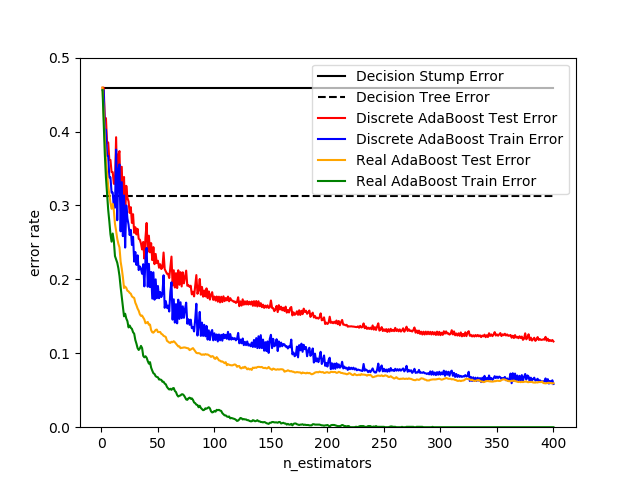
\includegraphics{wiki/1.png}
\caption{decision stump performance}
\end{figure}

On top of it we need to understand the difference between
\textbf{boosting} and \textbf{averaging}. Ensembles like AdaBoost,
SMOTEBoost, etc use weak classifiers and try to train them sequentially
which means further classifiers use the knowledge of previous
classifiers to perform better. This knowledge transfers via updating
weights of samples and modifying train data to each classifier.
Meanwhile, Averaging approaches such as RandomForest, train multiple
base classifiers independently and try to average their votes to get the
final output class.

Boosting enable ensemble to have low bias as each classifier learn to
work well on a part of feature space and small variance as the ensemble
average all classifiers hypotheses generated from different subsamples
of the data.

As we can see at the end of the notebook in visualization section,
RandomForest approach completely fail to capture minority data.

    \hypertarget{a-adaboost-m2}{%
\subsubsection{3.A AdaBoost M2}\label{a-adaboost-m2}}

This is the algorithm we use in SMOTEBoost, RUSBoost and RBBoost to
update weights and train classifiers. So all the lines here are also
available in the other ensembles with a tiny modification.

Note that in binary classification, AdaBoost M1 is identical to AdaBoost
M2 as they only differ for multiclass classification.

Here are the steps AdaBoost takes: 1. Consider uniform weight for all
samples in train set 2. Train a weak classifier given weights and whole
train set 3. Calculate a loss which is sum of the weights of all
misclassified instances in train set 4. Calculates Alpha term for weight
updating 5. Ignores classifier if it performs worse than random
classifier p \textless{}= 0.5 6. Decrease the weight of samples that
weak classifier predicted correctly by *Alpha. Decreasing weight of
correctly classified instances, enable the ensemble to learn instances
that are harder and previous weak classifiers failed to learn. It
increases generalization and introduces low-variance classifiers. 7. Go
to step 2 untill all classifiers in ensemble are trained 8. Use weighted
majority vote for inference time

    \begin{Verbatim}[commandchars=\\\{\}]
{\color{incolor}In [{\color{incolor}5}]:} \PY{k}{class} \PY{n+nc}{AdaBoostM2}\PY{p}{:}
            \PY{k}{def} \PY{n+nf}{\PYZus{}\PYZus{}init\PYZus{}\PYZus{}}\PY{p}{(}\PY{n+nb+bp}{self}\PY{p}{,} \PY{n}{x}\PY{p}{,} \PY{n}{y}\PY{p}{,} \PY{n}{n\PYZus{}classifier}\PY{p}{,} \PY{n}{base}\PY{o}{=}\PY{k+kc}{None}\PY{p}{,} \PY{n}{weights}\PY{o}{=}\PY{k+kc}{None}\PY{p}{,} \PY{o}{*}\PY{o}{*}\PY{n}{kwargs}\PY{p}{)}\PY{p}{:}
                \PY{l+s+sd}{\PYZdq{}\PYZdq{}\PYZdq{}}
        \PY{l+s+sd}{        Initialize AdaBoost M2 (Weight init is same as M1)}
        \PY{l+s+sd}{        }
        \PY{l+s+sd}{        :param x: input feauture in shape of (samples, features)}
        \PY{l+s+sd}{        :param y: input label in shape of (samples, )}
        \PY{l+s+sd}{        :param base: base classifier (default Decision Tree)}
        \PY{l+s+sd}{        :param n\PYZus{}classifier: number of base classifier in ensemble}
        \PY{l+s+sd}{        :param weights: init model with pretrained weights}
        \PY{l+s+sd}{        }
        \PY{l+s+sd}{        :return: A AdaBoost model}
        \PY{l+s+sd}{        \PYZdq{}\PYZdq{}\PYZdq{}}
                \PY{n+nb+bp}{self}\PY{o}{.}\PY{n}{x} \PY{o}{=} \PY{n}{x}
                \PY{n+nb+bp}{self}\PY{o}{.}\PY{n}{y} \PY{o}{=} \PY{n}{y}
                \PY{n+nb+bp}{self}\PY{o}{.}\PY{n}{base} \PY{o}{=} \PY{n}{base}
                \PY{k}{if} \PY{n+nb+bp}{self}\PY{o}{.}\PY{n}{base} \PY{o+ow}{is} \PY{k+kc}{None}\PY{p}{:}
                    \PY{n+nb+bp}{self}\PY{o}{.}\PY{n}{base} \PY{o}{=} \PY{n}{DecisionTreeClassifier}
                \PY{n+nb+bp}{self}\PY{o}{.}\PY{n}{n\PYZus{}classifier} \PY{o}{=} \PY{n}{n\PYZus{}classifier}
                \PY{n+nb+bp}{self}\PY{o}{.}\PY{n}{classifiers} \PY{o}{=} \PY{p}{[}\PY{p}{]}
                \PY{n+nb+bp}{self}\PY{o}{.}\PY{n}{weights} \PY{o}{=} \PY{n}{weights}
                \PY{n+nb+bp}{self}\PY{o}{.}\PY{n}{alpha} \PY{o}{=} \PY{p}{[}\PY{p}{]}
                \PY{n+nb+bp}{self}\PY{o}{.}\PY{n}{bad\PYZus{}classifier\PYZus{}idx} \PY{o}{=} \PY{p}{[}\PY{p}{]}
                
                \PY{c+c1}{\PYZsh{} init ensemble}
                \PY{k}{for} \PY{n}{n} \PY{o+ow}{in} \PY{n+nb}{range}\PY{p}{(}\PY{n+nb+bp}{self}\PY{o}{.}\PY{n}{n\PYZus{}classifier}\PY{p}{)}\PY{p}{:}
                    \PY{n+nb+bp}{self}\PY{o}{.}\PY{n}{classifiers}\PY{o}{.}\PY{n}{append}\PY{p}{(}\PY{n+nb+bp}{self}\PY{o}{.}\PY{n}{base}\PY{p}{(}\PY{o}{*}\PY{o}{*}\PY{n}{kwargs}\PY{p}{)}\PY{p}{)}
                
                \PY{k}{if} \PY{n+nb+bp}{self}\PY{o}{.}\PY{n}{weights} \PY{o+ow}{is} \PY{k+kc}{None}\PY{p}{:}
                    \PY{c+c1}{\PYZsh{} init weights using uniform distrobution}
                    \PY{n+nb+bp}{self}\PY{o}{.}\PY{n}{weights} \PY{o}{=} \PY{n}{np}\PY{o}{.}\PY{n}{ones}\PY{p}{(}\PY{n+nb}{len}\PY{p}{(}\PY{n+nb+bp}{self}\PY{o}{.}\PY{n}{x}\PY{p}{)}\PY{p}{)} \PY{o}{/} \PY{n+nb}{len}\PY{p}{(}\PY{n+nb+bp}{self}\PY{o}{.}\PY{n}{x}\PY{p}{)}
                    
            \PY{k}{def} \PY{n+nf}{predict}\PY{p}{(}\PY{n+nb+bp}{self}\PY{p}{,} \PY{n}{x}\PY{p}{)}\PY{p}{:}
                \PY{l+s+sd}{\PYZdq{}\PYZdq{}\PYZdq{}}
        \PY{l+s+sd}{        Predict the class of given instance}
        \PY{l+s+sd}{        }
        \PY{l+s+sd}{        :param x: input feauture in shape of (samples, features)}
        \PY{l+s+sd}{        }
        \PY{l+s+sd}{        :return: a prediction of classes in label encoded form with shape of (samples, )}
        \PY{l+s+sd}{        \PYZdq{}\PYZdq{}\PYZdq{}}
                
                \PY{n}{prediction} \PY{o}{=} \PY{n}{np}\PY{o}{.}\PY{n}{zeros}\PY{p}{(}\PY{p}{(}\PY{n+nb}{len}\PY{p}{(}\PY{n}{x}\PY{p}{)}\PY{p}{,}\PY{p}{)}\PY{p}{)}
                \PY{k}{for} \PY{n}{idx} \PY{o+ow}{in} \PY{n+nb}{range}\PY{p}{(}\PY{n+nb}{len}\PY{p}{(}\PY{n}{x}\PY{p}{)}\PY{p}{)}\PY{p}{:}
                    \PY{n}{prediction}\PY{p}{[}\PY{n}{idx}\PY{p}{]} \PY{o}{=} \PY{n+nb+bp}{self}\PY{o}{.}\PY{n}{\PYZus{}\PYZus{}predict\PYZus{}single\PYZus{}instance}\PY{p}{(}\PY{n}{x}\PY{p}{[}\PY{n}{idx}\PY{p}{]}\PY{o}{.}\PY{n}{reshape}\PY{p}{(}\PY{l+m+mi}{1}\PY{p}{,} \PY{o}{\PYZhy{}}\PY{l+m+mi}{1}\PY{p}{)}\PY{p}{)}
                \PY{k}{return} \PY{n}{prediction}
                    
            \PY{k}{def} \PY{n+nf}{\PYZus{}\PYZus{}predict\PYZus{}single\PYZus{}instance}\PY{p}{(}\PY{n+nb+bp}{self}\PY{p}{,} \PY{n}{x}\PY{p}{)}\PY{p}{:}
                \PY{l+s+sd}{\PYZdq{}\PYZdq{}\PYZdq{}}
        \PY{l+s+sd}{        Predict the class of given instance}
        \PY{l+s+sd}{        }
        \PY{l+s+sd}{        :param x: input feauture in shape of (1, features)}
        \PY{l+s+sd}{        }
        \PY{l+s+sd}{        :return: a prediction of classes in label encoded form with shape of (1, )}
        \PY{l+s+sd}{        \PYZdq{}\PYZdq{}\PYZdq{}}
                \PY{n}{p} \PY{o}{=} \PY{n}{np}\PY{o}{.}\PY{n}{zeros}\PY{p}{(}\PY{p}{(}\PY{l+m+mi}{1}\PY{p}{,} \PY{l+m+mi}{2}\PY{p}{)}\PY{p}{)}
                \PY{k}{for} \PY{n}{n} \PY{o+ow}{in} \PY{n+nb}{range}\PY{p}{(}\PY{n+nb+bp}{self}\PY{o}{.}\PY{n}{n\PYZus{}classifier}\PY{p}{)}\PY{p}{:}
                    \PY{k}{if} \PY{n}{n} \PY{o+ow}{not} \PY{o+ow}{in} \PY{n+nb+bp}{self}\PY{o}{.}\PY{n}{bad\PYZus{}classifier\PYZus{}idx}\PY{p}{:}
                        \PY{k}{if} \PY{n+nb+bp}{self}\PY{o}{.}\PY{n}{classifiers}\PY{p}{[}\PY{n}{n}\PY{p}{]}\PY{o}{.}\PY{n}{predict}\PY{p}{(}\PY{n}{x}\PY{p}{)} \PY{o}{==} \PY{l+m+mi}{1}\PY{p}{:}
                            \PY{n}{p}\PY{p}{[}\PY{l+m+mi}{0}\PY{p}{,}\PY{l+m+mi}{1}\PY{p}{]} \PY{o}{+}\PY{o}{=} \PY{n}{np}\PY{o}{.}\PY{n}{log}\PY{p}{(}\PY{l+m+mi}{1} \PY{o}{/} \PY{p}{(}\PY{n+nb+bp}{self}\PY{o}{.}\PY{n}{alpha}\PY{p}{[}\PY{n}{n}\PY{p}{]}\PY{o}{+}\PY{l+m+mf}{1e\PYZhy{}10}\PY{p}{)}\PY{p}{)}
                        \PY{k}{else}\PY{p}{:}
                            \PY{n}{p}\PY{p}{[}\PY{l+m+mi}{0}\PY{p}{,}\PY{l+m+mi}{0}\PY{p}{]} \PY{o}{+}\PY{o}{=} \PY{n}{np}\PY{o}{.}\PY{n}{log}\PY{p}{(}\PY{l+m+mi}{1} \PY{o}{/} \PY{p}{(}\PY{n+nb+bp}{self}\PY{o}{.}\PY{n}{alpha}\PY{p}{[}\PY{n}{n}\PY{p}{]}\PY{o}{+}\PY{l+m+mf}{1e\PYZhy{}10}\PY{p}{)}\PY{p}{)}
                \PY{n}{p}\PY{p}{[}\PY{p}{:}\PY{p}{,}\PY{l+m+mi}{1}\PY{p}{]} \PY{o}{+}\PY{o}{=} \PY{l+m+mf}{1e\PYZhy{}10} 
                \PY{k}{return} \PY{n}{np}\PY{o}{.}\PY{n}{argmax}\PY{p}{(}\PY{n}{p}\PY{p}{,} \PY{n}{axis}\PY{o}{=}\PY{l+m+mi}{1}\PY{p}{)}
            
            
            \PY{k}{def} \PY{n+nf}{fit}\PY{p}{(}\PY{n+nb+bp}{self}\PY{p}{)}\PY{p}{:}
                \PY{l+s+sd}{\PYZdq{}\PYZdq{}\PYZdq{}}
        \PY{l+s+sd}{        Train the ensemble using base weak classifiers}
        \PY{l+s+sd}{        \PYZdq{}\PYZdq{}\PYZdq{}}
                \PY{k}{for} \PY{n}{t} \PY{o+ow}{in} \PY{n+nb}{range}\PY{p}{(}\PY{n+nb+bp}{self}\PY{o}{.}\PY{n}{n\PYZus{}classifier}\PY{p}{)}\PY{p}{:}            
                    
                    \PY{c+c1}{\PYZsh{} training weak classifier}
                    \PY{n+nb+bp}{self}\PY{o}{.}\PY{n}{classifiers}\PY{p}{[}\PY{n}{t}\PY{p}{]}\PY{o}{.}\PY{n}{fit}\PY{p}{(}\PY{n+nb+bp}{self}\PY{o}{.}\PY{n}{x}\PY{p}{,} \PY{n+nb+bp}{self}\PY{o}{.}\PY{n}{y}\PY{p}{,} \PY{n}{sample\PYZus{}weight}\PY{o}{=}\PY{n+nb+bp}{self}\PY{o}{.}\PY{n}{weights}\PY{p}{)}
                                
                    \PY{c+c1}{\PYZsh{} calculating loss = sum of missclassified weights}
                    \PY{n}{miss\PYZus{}w} \PY{o}{=} \PY{n+nb+bp}{self}\PY{o}{.}\PY{n}{weights}\PY{p}{[}\PY{p}{(}\PY{n+nb+bp}{self}\PY{o}{.}\PY{n}{classifiers}\PY{p}{[}\PY{n}{t}\PY{p}{]}\PY{o}{.}\PY{n}{predict}\PY{p}{(}\PY{n+nb+bp}{self}\PY{o}{.}\PY{n}{x}\PY{p}{)} \PY{o}{!=} \PY{n+nb+bp}{self}\PY{o}{.}\PY{n}{y}\PY{p}{)}\PY{o}{.}\PY{n}{nonzero}\PY{p}{(}\PY{p}{)}\PY{p}{[}\PY{l+m+mi}{0}\PY{p}{]}\PY{p}{]}
                    \PY{n}{loss} \PY{o}{=} \PY{n}{np}\PY{o}{.}\PY{n}{sum}\PY{p}{(}\PY{n}{miss\PYZus{}w}\PY{p}{)} \PY{o}{/} \PY{l+m+mi}{2} 
                    
                    \PY{c+c1}{\PYZsh{} calculating beta}
                    \PY{n}{a} \PY{o}{=} \PY{n}{loss} \PY{o}{/} \PY{p}{(}\PY{l+m+mi}{1} \PY{o}{\PYZhy{}} \PY{n}{loss}\PY{p}{)}
                    \PY{n+nb+bp}{self}\PY{o}{.}\PY{n}{alpha}\PY{o}{.}\PY{n}{append}\PY{p}{(}\PY{n}{a}\PY{p}{)}
                    
                    \PY{c+c1}{\PYZsh{} drop classifiers with acc \PYZlt{} 0.5}
                    \PY{k}{if} \PY{n+nb+bp}{self}\PY{o}{.}\PY{n}{classifiers}\PY{p}{[}\PY{n}{t}\PY{p}{]}\PY{o}{.}\PY{n}{score}\PY{p}{(}\PY{n+nb+bp}{self}\PY{o}{.}\PY{n}{x}\PY{p}{,} \PY{n+nb+bp}{self}\PY{o}{.}\PY{n}{y}\PY{p}{)} \PY{o}{\PYZlt{}}\PY{o}{=} \PY{l+m+mf}{0.5}\PY{p}{:}
                        \PY{n+nb+bp}{self}\PY{o}{.}\PY{n}{bad\PYZus{}classifier\PYZus{}idx}\PY{o}{.}\PY{n}{append}\PY{p}{(}\PY{n}{t}\PY{p}{)}
                        \PY{k}{continue}
        
                    \PY{c+c1}{\PYZsh{} update weights}
                    \PY{n}{correct\PYZus{}pred\PYZus{}idx} \PY{o}{=} \PY{p}{(}\PY{n+nb+bp}{self}\PY{o}{.}\PY{n}{classifiers}\PY{p}{[}\PY{n}{t}\PY{p}{]}\PY{o}{.}\PY{n}{predict}\PY{p}{(}\PY{n+nb+bp}{self}\PY{o}{.}\PY{n}{x}\PY{p}{)} \PY{o}{==} \PY{n+nb+bp}{self}\PY{o}{.}\PY{n}{y}\PY{p}{)}\PY{o}{.}\PY{n}{nonzero}\PY{p}{(}\PY{p}{)}\PY{p}{[}\PY{l+m+mi}{0}\PY{p}{]}
                    \PY{n+nb+bp}{self}\PY{o}{.}\PY{n}{weights}\PY{p}{[}\PY{n}{correct\PYZus{}pred\PYZus{}idx}\PY{p}{]} \PY{o}{=} \PY{n+nb+bp}{self}\PY{o}{.}\PY{n}{weights}\PY{p}{[}\PY{n}{correct\PYZus{}pred\PYZus{}idx}\PY{p}{]} \PY{o}{*} \PY{n}{a}
                    
                    \PY{c+c1}{\PYZsh{} normalize weights}
                    \PY{n}{z} \PY{o}{=} \PY{n}{np}\PY{o}{.}\PY{n}{sum}\PY{p}{(}\PY{n+nb+bp}{self}\PY{o}{.}\PY{n}{weights}\PY{p}{)}
                    \PY{n+nb+bp}{self}\PY{o}{.}\PY{n}{weights} \PY{o}{=} \PY{n}{np}\PY{o}{.}\PY{n}{array}\PY{p}{(}\PY{p}{[}\PY{n}{w} \PY{o}{/} \PY{n}{z} \PY{k}{for} \PY{n}{w} \PY{o+ow}{in} \PY{n+nb+bp}{self}\PY{o}{.}\PY{n}{weights}\PY{p}{]}\PY{p}{)}
                     
            
            \PY{k}{def} \PY{n+nf}{score}\PY{p}{(}\PY{n+nb+bp}{self}\PY{p}{,} \PY{n}{x}\PY{p}{,} \PY{n}{y}\PY{p}{)}\PY{p}{:}
                \PY{n}{p} \PY{o}{=} \PY{n+nb+bp}{self}\PY{o}{.}\PY{n}{predict}\PY{p}{(}\PY{n}{x}\PY{p}{)}
                \PY{k}{return} \PY{n}{np}\PY{o}{.}\PY{n}{sum}\PY{p}{(}\PY{p}{(}\PY{n}{p} \PY{o}{==} \PY{n}{y}\PY{p}{)}\PY{o}{*}\PY{l+m+mi}{1}\PY{p}{)} \PY{o}{/} \PY{n+nb}{len}\PY{p}{(}\PY{n}{y}\PY{p}{)}   
        
        \PY{c+c1}{\PYZsh{} Test}
        \PY{c+c1}{\PYZsh{} model = AdaBoostM2(x=x\PYZus{}train, y=y\PYZus{}train, n\PYZus{}classifier=100, base=DecisionTreeClassifier, max\PYZus{}depth=1)}
        \PY{c+c1}{\PYZsh{} model.fit()}
        \PY{c+c1}{\PYZsh{} model.score(x\PYZus{}test, y\PYZus{}test)}
\end{Verbatim}


    \begin{Verbatim}[commandchars=\\\{\}]
{\color{incolor}In [{\color{incolor}6}]:} \PY{n}{adaboost\PYZus{}accuracies} \PY{o}{=} \PY{p}{[}\PY{p}{]}  \PY{c+c1}{\PYZsh{} accuracies of different ensembles given 5 folds}
        \PY{n}{adaboost\PYZus{}pr} \PY{o}{=} \PY{p}{[}\PY{p}{]}  \PY{c+c1}{\PYZsh{} precision\PYZhy{}recall of different ensebmles given 5 folds}
        \PY{n}{adaboost\PYZus{}auc} \PY{o}{=} \PY{p}{[}\PY{p}{]}  \PY{c+c1}{\PYZsh{} auc score of different ensebmles given 5 folds}
        \PY{n}{adaboost\PYZus{}roc} \PY{o}{=} \PY{p}{[}\PY{p}{]}  \PY{c+c1}{\PYZsh{} roc curve values of different ensebmles given 5 folds}
        
        \PY{k}{for} \PY{n}{es} \PY{o+ow}{in} \PY{n}{ensemble\PYZus{}sizes}\PY{p}{:}
            \PY{n}{kf\PYZus{}acc} \PY{o}{=} \PY{p}{[}\PY{p}{]}  \PY{c+c1}{\PYZsh{} accuracies of 5 folds}
            \PY{n}{kf\PYZus{}pr} \PY{o}{=} \PY{p}{[}\PY{p}{]}  \PY{c+c1}{\PYZsh{} precision\PYZhy{}recall of 5 folds}
            \PY{n}{kf\PYZus{}auc} \PY{o}{=} \PY{p}{[}\PY{p}{]}  \PY{c+c1}{\PYZsh{} auc of 5 folds}
            \PY{n}{kf\PYZus{}roc} \PY{o}{=} \PY{p}{[}\PY{p}{]}  \PY{c+c1}{\PYZsh{} roc of 5 folds}
            \PY{k}{for} \PY{n}{train\PYZus{}index}\PY{p}{,} \PY{n}{test\PYZus{}index} \PY{o+ow}{in} \PY{n}{kfold}\PY{o}{.}\PY{n}{split}\PY{p}{(}\PY{n}{x}\PY{p}{)}\PY{p}{:}
                \PY{n}{x\PYZus{}train}\PY{p}{,} \PY{n}{x\PYZus{}test} \PY{o}{=} \PY{n}{x}\PY{p}{[}\PY{n}{train\PYZus{}index}\PY{p}{]}\PY{p}{,} \PY{n}{x}\PY{p}{[}\PY{n}{test\PYZus{}index}\PY{p}{]}
                \PY{n}{y\PYZus{}train}\PY{p}{,} \PY{n}{y\PYZus{}test} \PY{o}{=} \PY{n}{y}\PY{p}{[}\PY{n}{train\PYZus{}index}\PY{p}{]}\PY{p}{,} \PY{n}{y}\PY{p}{[}\PY{n}{test\PYZus{}index}\PY{p}{]}
                \PY{n}{model} \PY{o}{=} \PY{n}{AdaBoostM2}\PY{p}{(}\PY{n}{x}\PY{o}{=}\PY{n}{x\PYZus{}train}\PY{p}{,} \PY{n}{y}\PY{o}{=}\PY{n}{y\PYZus{}train}\PY{p}{,} \PY{n}{n\PYZus{}classifier}\PY{o}{=}\PY{n}{es}\PY{p}{,} \PY{n}{base}\PY{o}{=}\PY{n}{DecisionTreeClassifier}\PY{p}{,} \PY{n}{max\PYZus{}depth}\PY{o}{=}\PY{l+m+mi}{1}\PY{p}{)}
                \PY{n}{model}\PY{o}{.}\PY{n}{fit}\PY{p}{(}\PY{p}{)}
                \PY{n}{y\PYZus{}pred} \PY{o}{=} \PY{n}{model}\PY{o}{.}\PY{n}{predict}\PY{p}{(}\PY{n}{x\PYZus{}test}\PY{p}{)}
                \PY{n}{p}\PY{p}{,} \PY{n}{r}\PY{p}{,} \PY{n}{\PYZus{}}\PY{p}{,} \PY{n}{\PYZus{}} \PY{o}{=} \PY{n}{precision\PYZus{}recall\PYZus{}fscore\PYZus{}support}\PY{p}{(}\PY{n}{y\PYZus{}test}\PY{p}{,} \PY{n}{y\PYZus{}pred}\PY{p}{,} \PY{n}{average}\PY{o}{=}\PY{l+s+s1}{\PYZsq{}}\PY{l+s+s1}{binary}\PY{l+s+s1}{\PYZsq{}}\PY{p}{)}
                \PY{n}{kf\PYZus{}pr}\PY{o}{.}\PY{n}{append}\PY{p}{(}\PY{p}{(}\PY{n}{p}\PY{p}{,} \PY{n}{r}\PY{p}{)}\PY{p}{)}
                \PY{n}{kf\PYZus{}acc}\PY{o}{.}\PY{n}{append}\PY{p}{(}\PY{n}{accuracy\PYZus{}score}\PY{p}{(}\PY{n}{y\PYZus{}test}\PY{p}{,} \PY{n}{y\PYZus{}pred}\PY{p}{)}\PY{p}{)}
                \PY{n}{kf\PYZus{}auc}\PY{o}{.}\PY{n}{append}\PY{p}{(}\PY{n}{roc\PYZus{}auc\PYZus{}score}\PY{p}{(}\PY{n}{y\PYZus{}test}\PY{p}{,} \PY{n}{y\PYZus{}pred}\PY{p}{,} \PY{n}{average}\PY{o}{=}\PY{l+s+s1}{\PYZsq{}}\PY{l+s+s1}{micro}\PY{l+s+s1}{\PYZsq{}}\PY{p}{)}\PY{p}{)}
                \PY{n}{kf\PYZus{}roc}\PY{o}{.}\PY{n}{append}\PY{p}{(}\PY{n}{roc\PYZus{}curve}\PY{p}{(}\PY{n}{y\PYZus{}test}\PY{p}{,} \PY{n}{y\PYZus{}pred}\PY{p}{,} \PY{n}{pos\PYZus{}label}\PY{o}{=}\PY{l+m+mi}{1}\PY{p}{)}\PY{p}{[}\PY{p}{:}\PY{o}{\PYZhy{}}\PY{l+m+mi}{1}\PY{p}{]}\PY{p}{)}
            \PY{n}{adaboost\PYZus{}auc}\PY{o}{.}\PY{n}{append}\PY{p}{(}\PY{n}{kf\PYZus{}auc}\PY{p}{)}
            \PY{n}{adaboost\PYZus{}roc}\PY{o}{.}\PY{n}{append}\PY{p}{(}\PY{n}{kf\PYZus{}roc}\PY{p}{)}
            \PY{n}{adaboost\PYZus{}pr}\PY{o}{.}\PY{n}{append}\PY{p}{(}\PY{n}{kf\PYZus{}pr}\PY{p}{)}
            \PY{n}{adaboost\PYZus{}accuracies}\PY{o}{.}\PY{n}{append}\PY{p}{(}\PY{n}{kf\PYZus{}acc}\PY{p}{)}
        \PY{k}{for} \PY{n}{idx}\PY{p}{,}\PY{n}{f} \PY{o+ow}{in} \PY{n+nb}{enumerate}\PY{p}{(}\PY{n}{adaboost\PYZus{}accuracies}\PY{p}{)}\PY{p}{:}
            \PY{n+nb}{print}\PY{p}{(}\PY{l+s+s1}{\PYZsq{}}\PY{l+s+s1}{Accuracy of ensemble with size of \PYZsh{}}\PY{l+s+si}{\PYZob{}\PYZcb{}}\PY{l+s+s1}{:}\PY{l+s+se}{\PYZbs{}n}\PY{l+s+s1}{ }\PY{l+s+si}{\PYZob{}\PYZcb{}}\PY{l+s+s1}{ \PYZhy{}\PYZhy{}\PYZhy{}\PYZgt{} AVG=}\PY{l+s+si}{\PYZob{}\PYZcb{}}\PY{l+s+s1}{\PYZsq{}}\PY{o}{.}\PY{n}{format}\PY{p}{(}
                \PY{n}{ensemble\PYZus{}sizes}\PY{p}{[}\PY{n}{idx}\PY{p}{]}\PY{p}{,} \PY{n}{f}\PY{p}{,} \PY{n}{np}\PY{o}{.}\PY{n}{mean}\PY{p}{(}\PY{n}{adaboost\PYZus{}accuracies}\PY{p}{[}\PY{n}{idx}\PY{p}{]}\PY{p}{)}\PY{p}{)}\PY{p}{)}
\end{Verbatim}


    \begin{Verbatim}[commandchars=\\\{\}]
Accuracy of ensemble with size of \#10:
 [0.95145631067961167, 0.91262135922330101, 0.970873786407767, 0.96116504854368934, 0.90196078431372551] ---> AVG=0.9396154578336189
Accuracy of ensemble with size of \#50:
 [0.95145631067961167, 0.91262135922330101, 0.970873786407767, 0.96116504854368934, 0.90196078431372551] ---> AVG=0.9396154578336189
Accuracy of ensemble with size of \#100:
 [0.95145631067961167, 0.91262135922330101, 0.970873786407767, 0.96116504854368934, 0.90196078431372551] ---> AVG=0.9396154578336189

    \end{Verbatim}

    \hypertarget{b-rusboost}{%
\subsubsection{3.B RUSBoost}\label{b-rusboost}}

RUSBoost uses same approach as is in AdaBoost but the only difference is
that AdaBoost uses all train data but RUSBoost uses \emph{Random Under
Sampling} technique which is simple term, it uses a subset of train data
each time to train weak classifiers but in the way that the balance of
minority and majority tend to be lower as we only select a random subset
of majority data. The method \texttt{\_\_undersample} is the
implementation of this approach.

In this implementation, at each iteration, a subset of majority data
with same size of minority data will be selected so each weak classifier
will be trained with same size of minority and majority data. (Random
sampling with replacement)

Here are the steps RUSBoost takes: 1. Consider uniform weight for all
samples in train set 2. Generate Random Under Sampling 1. Add all
minority samples to the new set \emph{S} 2. Add a unique subset of
majority data with same size as minority data to the set S 3. Train a
weak classifier given weights and subset sampled \emph{S} 4. Calculate a
loss which is sum of the weights of all misclassified instances in train
set 5. Calculates Alpha term for weight updating 6. Ignores classifier
if it performs worse than random classifier p \textless{}= 0.5 7.
Decrease the weight of samples that weak classifier predicted correctly
by *Alpha. 8. Go to step 2 untill all classifiers in ensemble are
trained 9. Use weighted majority vote for inference time

First obvious benefit of this approach is that in every iteration, we
feed same amount of minority and majority class to each classifier so
the classifiers will not be dominated by only majority class.

Another noticable feature of this algorithm is that it completely
outperforms AdaBoost and in some cases SMOTEBoost or comparable result,
it is much faster that SMOTEBoost and the algorithm is really simple to
implement.

RUS uses undersampling which the first drawback is loosing information
as we not using whole dataset. Meanwhile it decreases train time with
same ratio of majority to whole dataset. But as RUS is combined with
boosting feature, it enables to capture feature space well.

Although using RUS cause to classifier not to learn all feature space
very well because of information loss, boosing enables it to decrease
bias and capture most of the feature space.

Robustness to noise by using random sets.

Increasing \emph{diversity} by working on data level.

    \begin{Verbatim}[commandchars=\\\{\}]
{\color{incolor}In [{\color{incolor}6}]:} \PY{k}{class} \PY{n+nc}{RUSBoost}\PY{p}{:}
            \PY{k}{def} \PY{n+nf}{\PYZus{}\PYZus{}init\PYZus{}\PYZus{}}\PY{p}{(}\PY{n+nb+bp}{self}\PY{p}{,} \PY{n}{x}\PY{p}{,} \PY{n}{y}\PY{p}{,} \PY{n}{n\PYZus{}classifier}\PY{p}{,} \PY{n}{base}\PY{o}{=}\PY{k+kc}{None}\PY{p}{,} \PY{n}{weights}\PY{o}{=}\PY{k+kc}{None}\PY{p}{,} \PY{o}{*}\PY{o}{*}\PY{n}{kwargs}\PY{p}{)}\PY{p}{:}
                \PY{l+s+sd}{\PYZdq{}\PYZdq{}\PYZdq{}}
        \PY{l+s+sd}{        Initialize RUSBoost}
        \PY{l+s+sd}{        }
        \PY{l+s+sd}{        :param x: input feauture in shape of (samples, features)}
        \PY{l+s+sd}{        :param y: input label in shape of (samples, )}
        \PY{l+s+sd}{        :param base: base classifier (default Decision Tree)}
        \PY{l+s+sd}{        :param n\PYZus{}classifier: number of base classifier in ensemble}
        \PY{l+s+sd}{        :param weights: init model with pretrained weights}
        \PY{l+s+sd}{        }
        \PY{l+s+sd}{        :return: A RUSBoost model}
        \PY{l+s+sd}{        \PYZdq{}\PYZdq{}\PYZdq{}}
                \PY{n+nb+bp}{self}\PY{o}{.}\PY{n}{x} \PY{o}{=} \PY{n}{x}
                \PY{n+nb+bp}{self}\PY{o}{.}\PY{n}{y} \PY{o}{=} \PY{n}{y}
                \PY{n+nb+bp}{self}\PY{o}{.}\PY{n}{base} \PY{o}{=} \PY{n}{base}
                \PY{k}{if} \PY{n+nb+bp}{self}\PY{o}{.}\PY{n}{base} \PY{o+ow}{is} \PY{k+kc}{None}\PY{p}{:}
                    \PY{n+nb+bp}{self}\PY{o}{.}\PY{n}{base} \PY{o}{=} \PY{n}{DecisionTreeClassifier}
                \PY{n+nb+bp}{self}\PY{o}{.}\PY{n}{n\PYZus{}classifier} \PY{o}{=} \PY{n}{n\PYZus{}classifier}
                \PY{n+nb+bp}{self}\PY{o}{.}\PY{n}{classifiers} \PY{o}{=} \PY{p}{[}\PY{p}{]}
                \PY{n+nb+bp}{self}\PY{o}{.}\PY{n}{weights} \PY{o}{=} \PY{n}{weights}
                \PY{n+nb+bp}{self}\PY{o}{.}\PY{n}{alpha} \PY{o}{=} \PY{p}{[}\PY{p}{]}
                \PY{n+nb+bp}{self}\PY{o}{.}\PY{n}{bad\PYZus{}classifier\PYZus{}idx} \PY{o}{=} \PY{p}{[}\PY{p}{]}
                
                \PY{c+c1}{\PYZsh{} init ensemble}
                \PY{k}{for} \PY{n}{n} \PY{o+ow}{in} \PY{n+nb}{range}\PY{p}{(}\PY{n+nb+bp}{self}\PY{o}{.}\PY{n}{n\PYZus{}classifier}\PY{p}{)}\PY{p}{:}
                    \PY{n+nb+bp}{self}\PY{o}{.}\PY{n}{classifiers}\PY{o}{.}\PY{n}{append}\PY{p}{(}\PY{n+nb+bp}{self}\PY{o}{.}\PY{n}{base}\PY{p}{(}\PY{o}{*}\PY{o}{*}\PY{n}{kwargs}\PY{p}{)}\PY{p}{)}
                
                \PY{k}{if} \PY{n+nb+bp}{self}\PY{o}{.}\PY{n}{weights} \PY{o+ow}{is} \PY{k+kc}{None}\PY{p}{:}
                    \PY{c+c1}{\PYZsh{} init weights using uniform distrobution}
                    \PY{n+nb+bp}{self}\PY{o}{.}\PY{n}{weights} \PY{o}{=} \PY{n}{np}\PY{o}{.}\PY{n}{ones}\PY{p}{(}\PY{p}{(}\PY{n+nb}{len}\PY{p}{(}\PY{n+nb+bp}{self}\PY{o}{.}\PY{n}{x}\PY{p}{)}\PY{p}{)}\PY{p}{)} \PY{o}{/} \PY{n+nb}{len}\PY{p}{(}\PY{n+nb+bp}{self}\PY{o}{.}\PY{n}{x}\PY{p}{)}
                    
            \PY{k}{def} \PY{n+nf}{predict}\PY{p}{(}\PY{n+nb+bp}{self}\PY{p}{,} \PY{n}{x}\PY{p}{)}\PY{p}{:}
                \PY{l+s+sd}{\PYZdq{}\PYZdq{}\PYZdq{}}
        \PY{l+s+sd}{        Predict the class of given instance}
        \PY{l+s+sd}{        }
        \PY{l+s+sd}{        :param x: input feauture in shape of (samples, features)}
        \PY{l+s+sd}{        }
        \PY{l+s+sd}{        :return: a prediction of classes in label encoded form with shape of (samples, )}
        \PY{l+s+sd}{        \PYZdq{}\PYZdq{}\PYZdq{}}
                
                \PY{n}{prediction} \PY{o}{=} \PY{n}{np}\PY{o}{.}\PY{n}{zeros}\PY{p}{(}\PY{p}{(}\PY{n+nb}{len}\PY{p}{(}\PY{n}{x}\PY{p}{)}\PY{p}{,}\PY{p}{)}\PY{p}{)}
                \PY{k}{for} \PY{n}{idx} \PY{o+ow}{in} \PY{n+nb}{range}\PY{p}{(}\PY{n+nb}{len}\PY{p}{(}\PY{n}{x}\PY{p}{)}\PY{p}{)}\PY{p}{:}
                    \PY{n}{prediction}\PY{p}{[}\PY{n}{idx}\PY{p}{]} \PY{o}{=} \PY{n+nb+bp}{self}\PY{o}{.}\PY{n}{\PYZus{}\PYZus{}predict\PYZus{}single\PYZus{}instance}\PY{p}{(}\PY{n}{x}\PY{p}{[}\PY{n}{idx}\PY{p}{]}\PY{o}{.}\PY{n}{reshape}\PY{p}{(}\PY{l+m+mi}{1}\PY{p}{,} \PY{o}{\PYZhy{}}\PY{l+m+mi}{1}\PY{p}{)}\PY{p}{)}
                \PY{k}{return} \PY{n}{prediction}
                    
            \PY{k}{def} \PY{n+nf}{\PYZus{}\PYZus{}predict\PYZus{}single\PYZus{}instance}\PY{p}{(}\PY{n+nb+bp}{self}\PY{p}{,} \PY{n}{x}\PY{p}{)}\PY{p}{:}
                \PY{l+s+sd}{\PYZdq{}\PYZdq{}\PYZdq{}}
        \PY{l+s+sd}{        Predict the class of given instance}
        \PY{l+s+sd}{        }
        \PY{l+s+sd}{        :param x: input feauture in shape of (1, features)}
        \PY{l+s+sd}{        }
        \PY{l+s+sd}{        :return: a prediction of classes in label encoded form with shape of (1, )}
        \PY{l+s+sd}{        \PYZdq{}\PYZdq{}\PYZdq{}}
                \PY{n}{p} \PY{o}{=} \PY{n}{np}\PY{o}{.}\PY{n}{zeros}\PY{p}{(}\PY{p}{(}\PY{l+m+mi}{1}\PY{p}{,} \PY{l+m+mi}{2}\PY{p}{)}\PY{p}{)}
                \PY{k}{for} \PY{n}{n} \PY{o+ow}{in} \PY{n+nb}{range}\PY{p}{(}\PY{n+nb+bp}{self}\PY{o}{.}\PY{n}{n\PYZus{}classifier}\PY{p}{)}\PY{p}{:}
                    \PY{k}{if} \PY{n}{n} \PY{o+ow}{not} \PY{o+ow}{in} \PY{n+nb+bp}{self}\PY{o}{.}\PY{n}{bad\PYZus{}classifier\PYZus{}idx}\PY{p}{:}
                        \PY{k}{if} \PY{n+nb+bp}{self}\PY{o}{.}\PY{n}{classifiers}\PY{p}{[}\PY{n}{n}\PY{p}{]}\PY{o}{.}\PY{n}{predict}\PY{p}{(}\PY{n}{x}\PY{p}{)} \PY{o}{==} \PY{l+m+mi}{1}\PY{p}{:}
                            \PY{n}{p}\PY{p}{[}\PY{l+m+mi}{0}\PY{p}{,}\PY{l+m+mi}{1}\PY{p}{]} \PY{o}{+}\PY{o}{=} \PY{n}{np}\PY{o}{.}\PY{n}{log}\PY{p}{(}\PY{l+m+mi}{1} \PY{o}{/} \PY{p}{(}\PY{n+nb+bp}{self}\PY{o}{.}\PY{n}{alpha}\PY{p}{[}\PY{n}{n}\PY{p}{]}\PY{o}{+}\PY{l+m+mf}{1e\PYZhy{}10}\PY{p}{)}\PY{p}{)}
                        \PY{k}{else}\PY{p}{:}
                            \PY{n}{p}\PY{p}{[}\PY{l+m+mi}{0}\PY{p}{,}\PY{l+m+mi}{0}\PY{p}{]} \PY{o}{+}\PY{o}{=} \PY{n}{np}\PY{o}{.}\PY{n}{log}\PY{p}{(}\PY{l+m+mi}{1} \PY{o}{/} \PY{p}{(}\PY{n+nb+bp}{self}\PY{o}{.}\PY{n}{alpha}\PY{p}{[}\PY{n}{n}\PY{p}{]}\PY{o}{+}\PY{l+m+mf}{1e\PYZhy{}10}\PY{p}{)}\PY{p}{)}
                \PY{n}{p}\PY{p}{[}\PY{p}{:}\PY{p}{,}\PY{l+m+mi}{1}\PY{p}{]} \PY{o}{+}\PY{o}{=} \PY{l+m+mf}{1e\PYZhy{}10}
                \PY{k}{return} \PY{n}{np}\PY{o}{.}\PY{n}{argmax}\PY{p}{(}\PY{n}{p}\PY{p}{,} \PY{n}{axis}\PY{o}{=}\PY{l+m+mi}{1}\PY{p}{)}
            
            
            \PY{k}{def} \PY{n+nf}{fit}\PY{p}{(}\PY{n+nb+bp}{self}\PY{p}{)}\PY{p}{:}
                \PY{l+s+sd}{\PYZdq{}\PYZdq{}\PYZdq{}}
        \PY{l+s+sd}{        Train the ensemble using RUS data boosting and base weak classifiers}
        \PY{l+s+sd}{        \PYZdq{}\PYZdq{}\PYZdq{}}
                \PY{k}{for} \PY{n}{t} \PY{o+ow}{in} \PY{n+nb}{range}\PY{p}{(}\PY{n+nb+bp}{self}\PY{o}{.}\PY{n}{n\PYZus{}classifier}\PY{p}{)}\PY{p}{:}            
                    \PY{c+c1}{\PYZsh{} random under sampling}
                    \PY{n}{rus\PYZus{}idx} \PY{o}{=} \PY{n+nb+bp}{self}\PY{o}{.}\PY{n}{\PYZus{}\PYZus{}undersample}\PY{p}{(}\PY{p}{)}
        
                    \PY{c+c1}{\PYZsh{} training weak classifier}
                    \PY{n+nb+bp}{self}\PY{o}{.}\PY{n}{classifiers}\PY{p}{[}\PY{n}{t}\PY{p}{]}\PY{o}{.}\PY{n}{fit}\PY{p}{(}\PY{n+nb+bp}{self}\PY{o}{.}\PY{n}{x}\PY{p}{[}\PY{n}{rus\PYZus{}idx}\PY{p}{]}\PY{p}{,} \PY{n+nb+bp}{self}\PY{o}{.}\PY{n}{y}\PY{p}{[}\PY{n}{rus\PYZus{}idx}\PY{p}{]}\PY{p}{,} \PY{n+nb+bp}{self}\PY{o}{.}\PY{n}{weights}\PY{p}{[}\PY{n}{rus\PYZus{}idx}\PY{p}{]}\PY{p}{)}
                    
                    \PY{c+c1}{\PYZsh{} calculating loss = sum of missclassified weights            }
                    \PY{n}{miss\PYZus{}w} \PY{o}{=} \PY{n+nb+bp}{self}\PY{o}{.}\PY{n}{weights}\PY{p}{[}\PY{p}{(}\PY{n+nb+bp}{self}\PY{o}{.}\PY{n}{classifiers}\PY{p}{[}\PY{n}{t}\PY{p}{]}\PY{o}{.}\PY{n}{predict}\PY{p}{(}\PY{n+nb+bp}{self}\PY{o}{.}\PY{n}{x}\PY{p}{)} \PY{o}{!=} \PY{n+nb+bp}{self}\PY{o}{.}\PY{n}{y}\PY{p}{)}\PY{o}{.}\PY{n}{nonzero}\PY{p}{(}\PY{p}{)}\PY{p}{[}\PY{l+m+mi}{0}\PY{p}{]}\PY{p}{]}
                    \PY{n}{loss} \PY{o}{=} \PY{n}{np}\PY{o}{.}\PY{n}{sum}\PY{p}{(}\PY{n}{miss\PYZus{}w}\PY{p}{)} \PY{o}{/} \PY{l+m+mi}{2} 
                    
                    \PY{c+c1}{\PYZsh{} calculating beta}
                    \PY{n}{a} \PY{o}{=} \PY{n}{loss} \PY{o}{/} \PY{p}{(}\PY{l+m+mi}{1} \PY{o}{\PYZhy{}} \PY{n}{loss}\PY{p}{)}
                    \PY{n+nb+bp}{self}\PY{o}{.}\PY{n}{alpha}\PY{o}{.}\PY{n}{append}\PY{p}{(}\PY{n}{a}\PY{p}{)}
                    
                    \PY{c+c1}{\PYZsh{} drop bad classifiers}
                    \PY{k}{if} \PY{n+nb+bp}{self}\PY{o}{.}\PY{n}{classifiers}\PY{p}{[}\PY{n}{t}\PY{p}{]}\PY{o}{.}\PY{n}{score}\PY{p}{(}\PY{n+nb+bp}{self}\PY{o}{.}\PY{n}{x}\PY{p}{,} \PY{n+nb+bp}{self}\PY{o}{.}\PY{n}{y}\PY{p}{)} \PY{o}{\PYZlt{}}\PY{o}{=} \PY{l+m+mf}{0.5}\PY{p}{:}
                        \PY{n+nb+bp}{self}\PY{o}{.}\PY{n}{bad\PYZus{}classifier\PYZus{}idx}\PY{o}{.}\PY{n}{append}\PY{p}{(}\PY{n}{t}\PY{p}{)}
                        \PY{k}{continue}
                    
                    \PY{c+c1}{\PYZsh{} update weights}
                    \PY{n}{correct\PYZus{}pred\PYZus{}idx} \PY{o}{=} \PY{p}{(}\PY{n+nb+bp}{self}\PY{o}{.}\PY{n}{classifiers}\PY{p}{[}\PY{n}{t}\PY{p}{]}\PY{o}{.}\PY{n}{predict}\PY{p}{(}\PY{n+nb+bp}{self}\PY{o}{.}\PY{n}{x}\PY{p}{)} \PY{o}{==} \PY{n+nb+bp}{self}\PY{o}{.}\PY{n}{y}\PY{p}{)}\PY{o}{.}\PY{n}{nonzero}\PY{p}{(}\PY{p}{)}\PY{p}{[}\PY{l+m+mi}{0}\PY{p}{]}
                    \PY{n+nb+bp}{self}\PY{o}{.}\PY{n}{weights}\PY{p}{[}\PY{n}{correct\PYZus{}pred\PYZus{}idx}\PY{p}{]} \PY{o}{=} \PY{n+nb+bp}{self}\PY{o}{.}\PY{n}{weights}\PY{p}{[}\PY{n}{correct\PYZus{}pred\PYZus{}idx}\PY{p}{]} \PY{o}{*} \PY{n}{a}
                    
                    \PY{c+c1}{\PYZsh{} normalize weights}
                    \PY{n}{z} \PY{o}{=} \PY{n}{np}\PY{o}{.}\PY{n}{sum}\PY{p}{(}\PY{n+nb+bp}{self}\PY{o}{.}\PY{n}{weights}\PY{p}{)}
                    \PY{n+nb+bp}{self}\PY{o}{.}\PY{n}{weights} \PY{o}{=} \PY{n}{np}\PY{o}{.}\PY{n}{array}\PY{p}{(}\PY{p}{[}\PY{n}{w} \PY{o}{/} \PY{n}{z} \PY{k}{for} \PY{n}{w} \PY{o+ow}{in} \PY{n+nb+bp}{self}\PY{o}{.}\PY{n}{weights}\PY{p}{]}\PY{p}{)}
                     
            
            \PY{k}{def} \PY{n+nf}{score}\PY{p}{(}\PY{n+nb+bp}{self}\PY{p}{,} \PY{n}{x}\PY{p}{,} \PY{n}{y}\PY{p}{)}\PY{p}{:}
                \PY{n}{p} \PY{o}{=} \PY{n+nb+bp}{self}\PY{o}{.}\PY{n}{predict}\PY{p}{(}\PY{n}{x}\PY{p}{)}
                \PY{k}{return} \PY{p}{(}\PY{n}{p} \PY{o}{==} \PY{n}{y}\PY{p}{)}\PY{o}{.}\PY{n}{nonzero}\PY{p}{(}\PY{p}{)}\PY{p}{[}\PY{l+m+mi}{0}\PY{p}{]}\PY{o}{.}\PY{n+nf+fm}{\PYZus{}\PYZus{}len\PYZus{}\PYZus{}}\PY{p}{(}\PY{p}{)} \PY{o}{/} \PY{n+nb}{len}\PY{p}{(}\PY{n}{y}\PY{p}{)}
                   
            \PY{k}{def} \PY{n+nf}{\PYZus{}\PYZus{}undersample}\PY{p}{(}\PY{n+nb+bp}{self}\PY{p}{)}\PY{p}{:}
                \PY{l+s+sd}{\PYZdq{}\PYZdq{}\PYZdq{}}
        \PY{l+s+sd}{        Generates a random unique subset of majority data as same size as minority and return the indices}
        \PY{l+s+sd}{        }
        \PY{l+s+sd}{        :return: A sorted list of indices with shape of (2*minority\PYZus{}data, )}
        \PY{l+s+sd}{        \PYZdq{}\PYZdq{}\PYZdq{}}
                \PY{n}{pos\PYZus{}size} \PY{o}{=} \PY{n+nb}{len}\PY{p}{(}\PY{p}{(}\PY{n+nb+bp}{self}\PY{o}{.}\PY{n}{y}\PY{o}{==}\PY{l+m+mi}{1}\PY{p}{)}\PY{o}{.}\PY{n}{nonzero}\PY{p}{(}\PY{p}{)}\PY{p}{[}\PY{l+m+mi}{0}\PY{p}{]}\PY{p}{)}
                \PY{n}{neg\PYZus{}size} \PY{o}{=} \PY{n+nb}{len}\PY{p}{(}\PY{p}{(}\PY{n+nb+bp}{self}\PY{o}{.}\PY{n}{y}\PY{o}{==}\PY{l+m+mi}{0}\PY{p}{)}\PY{o}{.}\PY{n}{nonzero}\PY{p}{(}\PY{p}{)}\PY{p}{[}\PY{l+m+mi}{0}\PY{p}{]}\PY{p}{)}
                \PY{n}{pos\PYZus{}data} \PY{o}{=} \PY{n+nb+bp}{self}\PY{o}{.}\PY{n}{x}\PY{p}{[}\PY{n+nb+bp}{self}\PY{o}{.}\PY{n}{y}\PY{o}{==}\PY{l+m+mi}{1}\PY{p}{]}
                \PY{n}{neg\PYZus{}data} \PY{o}{=} \PY{n+nb+bp}{self}\PY{o}{.}\PY{n}{x}\PY{p}{[}\PY{n+nb+bp}{self}\PY{o}{.}\PY{n}{y}\PY{o}{==}\PY{l+m+mi}{0}\PY{p}{]}
                
                \PY{k}{if} \PY{n}{pos\PYZus{}size} \PY{o}{\PYZgt{}} \PY{n}{neg\PYZus{}size}\PY{p}{:}
                    \PY{n+nb+bp}{self}\PY{o}{.}\PY{n}{major\PYZus{}data} \PY{o}{=} \PY{n}{pos\PYZus{}data}
                    \PY{n+nb+bp}{self}\PY{o}{.}\PY{n}{minor\PYZus{}data} \PY{o}{=} \PY{n}{neg\PYZus{}data}
                    \PY{n+nb+bp}{self}\PY{o}{.}\PY{n}{minor} \PY{o}{=} \PY{l+m+mi}{0}
                \PY{k}{else}\PY{p}{:}
                    \PY{n+nb+bp}{self}\PY{o}{.}\PY{n}{minor\PYZus{}data} \PY{o}{=} \PY{n}{pos\PYZus{}data}
                    \PY{n+nb+bp}{self}\PY{o}{.}\PY{n}{major\PYZus{}data} \PY{o}{=} \PY{n}{neg\PYZus{}data}
                    \PY{n+nb+bp}{self}\PY{o}{.}\PY{n}{minor} \PY{o}{=} \PY{l+m+mi}{1}
                \PY{c+c1}{\PYZsh{} getting index of sampled intances for enabling correct weight update}
                \PY{n}{minor\PYZus{}idx} \PY{o}{=} \PY{p}{(}\PY{n+nb+bp}{self}\PY{o}{.}\PY{n}{y} \PY{o}{==} \PY{n+nb+bp}{self}\PY{o}{.}\PY{n}{minor}\PY{p}{)}\PY{o}{.}\PY{n}{nonzero}\PY{p}{(}\PY{p}{)}\PY{p}{[}\PY{l+m+mi}{0}\PY{p}{]}
                \PY{n}{major\PYZus{}idx} \PY{o}{=} \PY{p}{(}\PY{n+nb+bp}{self}\PY{o}{.}\PY{n}{y} \PY{o}{==} \PY{n+nb}{int}\PY{p}{(}\PY{o+ow}{not} \PY{n+nb+bp}{self}\PY{o}{.}\PY{n}{minor}\PY{p}{)}\PY{p}{)}\PY{o}{.}\PY{n}{nonzero}\PY{p}{(}\PY{p}{)}\PY{p}{[}\PY{l+m+mi}{0}\PY{p}{]}
                \PY{n}{major\PYZus{}idx} \PY{o}{=} \PY{n}{np}\PY{o}{.}\PY{n}{array}\PY{p}{(}\PY{n}{random}\PY{o}{.}\PY{n}{sample}\PY{p}{(}\PY{n+nb}{list}\PY{p}{(}\PY{n}{major\PYZus{}idx}\PY{p}{)}\PY{p}{,} \PY{n+nb}{len}\PY{p}{(}\PY{n+nb+bp}{self}\PY{o}{.}\PY{n}{minor\PYZus{}data}\PY{p}{)}\PY{p}{)}\PY{p}{)}
                \PY{k}{return} \PY{n+nb}{sorted}\PY{p}{(}\PY{n}{np}\PY{o}{.}\PY{n}{concatenate}\PY{p}{(}\PY{p}{(}\PY{n}{minor\PYZus{}idx}\PY{p}{,} \PY{n}{major\PYZus{}idx}\PY{p}{)}\PY{p}{)}\PY{p}{)}
            
        \PY{c+c1}{\PYZsh{} test}
        \PY{c+c1}{\PYZsh{} model = RUSBoost(x=x\PYZus{}train, y=y\PYZus{}train, n\PYZus{}classifier=30, base=DecisionTreeClassifier, max\PYZus{}depth=1)}
        \PY{c+c1}{\PYZsh{} model.fit()}
        \PY{c+c1}{\PYZsh{} model.score(x\PYZus{}test, y\PYZus{}test)}
\end{Verbatim}


    \begin{Verbatim}[commandchars=\\\{\}]
{\color{incolor}In [{\color{incolor}8}]:} \PY{n}{rusboost\PYZus{}accuracies} \PY{o}{=} \PY{p}{[}\PY{p}{]}  \PY{c+c1}{\PYZsh{} accuracies of different ensembles given 5 folds}
        \PY{n}{rusboost\PYZus{}pr} \PY{o}{=} \PY{p}{[}\PY{p}{]}
        \PY{n}{rusboost\PYZus{}roc} \PY{o}{=} \PY{p}{[}\PY{p}{]}
        \PY{n}{rusboost\PYZus{}auc} \PY{o}{=} \PY{p}{[}\PY{p}{]}
        
        \PY{k}{for} \PY{n}{es} \PY{o+ow}{in} \PY{n}{ensemble\PYZus{}sizes}\PY{p}{:}
            \PY{n}{kf\PYZus{}acc} \PY{o}{=} \PY{p}{[}\PY{p}{]}  \PY{c+c1}{\PYZsh{} accuracies of 5 fold}
            \PY{n}{kf\PYZus{}pr} \PY{o}{=} \PY{p}{[}\PY{p}{]}
            \PY{n}{kf\PYZus{}auc} \PY{o}{=} \PY{p}{[}\PY{p}{]}  \PY{c+c1}{\PYZsh{} auc of 5 folds}
            \PY{n}{kf\PYZus{}roc} \PY{o}{=} \PY{p}{[}\PY{p}{]}  \PY{c+c1}{\PYZsh{} roc of 5 folds}
            \PY{k}{for} \PY{n}{train\PYZus{}index}\PY{p}{,} \PY{n}{test\PYZus{}index} \PY{o+ow}{in} \PY{n}{kfold}\PY{o}{.}\PY{n}{split}\PY{p}{(}\PY{n}{x}\PY{p}{)}\PY{p}{:}
                \PY{n}{x\PYZus{}train}\PY{p}{,} \PY{n}{x\PYZus{}test} \PY{o}{=} \PY{n}{x}\PY{p}{[}\PY{n}{train\PYZus{}index}\PY{p}{]}\PY{p}{,} \PY{n}{x}\PY{p}{[}\PY{n}{test\PYZus{}index}\PY{p}{]}
                \PY{n}{y\PYZus{}train}\PY{p}{,} \PY{n}{y\PYZus{}test} \PY{o}{=} \PY{n}{y}\PY{p}{[}\PY{n}{train\PYZus{}index}\PY{p}{]}\PY{p}{,} \PY{n}{y}\PY{p}{[}\PY{n}{test\PYZus{}index}\PY{p}{]}
                \PY{n}{model} \PY{o}{=} \PY{n}{RUSBoost}\PY{p}{(}\PY{n}{x}\PY{o}{=}\PY{n}{x\PYZus{}train}\PY{p}{,} \PY{n}{y}\PY{o}{=}\PY{n}{y\PYZus{}train}\PY{p}{,} \PY{n}{n\PYZus{}classifier}\PY{o}{=}\PY{n}{es}\PY{p}{,} \PY{n}{base}\PY{o}{=}\PY{n}{DecisionTreeClassifier}\PY{p}{,} \PY{n}{max\PYZus{}depth}\PY{o}{=}\PY{l+m+mi}{1}\PY{p}{)}
                \PY{n}{model}\PY{o}{.}\PY{n}{fit}\PY{p}{(}\PY{p}{)}
                \PY{n}{y\PYZus{}pred} \PY{o}{=} \PY{n}{model}\PY{o}{.}\PY{n}{predict}\PY{p}{(}\PY{n}{x\PYZus{}test}\PY{p}{)}
                \PY{n}{p}\PY{p}{,} \PY{n}{r}\PY{p}{,} \PY{n}{\PYZus{}}\PY{p}{,} \PY{n}{\PYZus{}} \PY{o}{=} \PY{n}{precision\PYZus{}recall\PYZus{}fscore\PYZus{}support}\PY{p}{(}\PY{n}{y\PYZus{}test}\PY{p}{,} \PY{n}{y\PYZus{}pred}\PY{p}{,} \PY{n}{average}\PY{o}{=}\PY{l+s+s1}{\PYZsq{}}\PY{l+s+s1}{binary}\PY{l+s+s1}{\PYZsq{}}\PY{p}{)}
                \PY{n}{kf\PYZus{}pr}\PY{o}{.}\PY{n}{append}\PY{p}{(}\PY{p}{(}\PY{n}{p}\PY{p}{,} \PY{n}{r}\PY{p}{)}\PY{p}{)}
                \PY{n}{kf\PYZus{}acc}\PY{o}{.}\PY{n}{append}\PY{p}{(}\PY{n}{accuracy\PYZus{}score}\PY{p}{(}\PY{n}{y\PYZus{}test}\PY{p}{,} \PY{n}{y\PYZus{}pred}\PY{p}{)}\PY{p}{)}
                \PY{n}{kf\PYZus{}auc}\PY{o}{.}\PY{n}{append}\PY{p}{(}\PY{n}{roc\PYZus{}auc\PYZus{}score}\PY{p}{(}\PY{n}{y\PYZus{}test}\PY{p}{,} \PY{n}{y\PYZus{}pred}\PY{p}{,} \PY{n}{average}\PY{o}{=}\PY{l+s+s1}{\PYZsq{}}\PY{l+s+s1}{micro}\PY{l+s+s1}{\PYZsq{}}\PY{p}{)}\PY{p}{)}
                \PY{n}{kf\PYZus{}roc}\PY{o}{.}\PY{n}{append}\PY{p}{(}\PY{n}{roc\PYZus{}curve}\PY{p}{(}\PY{n}{y\PYZus{}test}\PY{p}{,} \PY{n}{y\PYZus{}pred}\PY{p}{,} \PY{n}{pos\PYZus{}label}\PY{o}{=}\PY{l+m+mi}{1}\PY{p}{)}\PY{p}{[}\PY{p}{:}\PY{o}{\PYZhy{}}\PY{l+m+mi}{1}\PY{p}{]}\PY{p}{)}
            \PY{n}{rusboost\PYZus{}auc}\PY{o}{.}\PY{n}{append}\PY{p}{(}\PY{n}{kf\PYZus{}auc}\PY{p}{)}
            \PY{n}{rusboost\PYZus{}roc}\PY{o}{.}\PY{n}{append}\PY{p}{(}\PY{n}{kf\PYZus{}roc}\PY{p}{)}
            \PY{n}{rusboost\PYZus{}pr}\PY{o}{.}\PY{n}{append}\PY{p}{(}\PY{n}{kf\PYZus{}pr}\PY{p}{)}
            \PY{n}{rusboost\PYZus{}accuracies}\PY{o}{.}\PY{n}{append}\PY{p}{(}\PY{n}{kf\PYZus{}acc}\PY{p}{)}
        \PY{k}{for} \PY{n}{idx}\PY{p}{,}\PY{n}{f} \PY{o+ow}{in} \PY{n+nb}{enumerate}\PY{p}{(}\PY{n}{rusboost\PYZus{}accuracies}\PY{p}{)}\PY{p}{:}
            \PY{n+nb}{print}\PY{p}{(}\PY{l+s+s1}{\PYZsq{}}\PY{l+s+s1}{Accuracy of ensemble with size of \PYZsh{}}\PY{l+s+si}{\PYZob{}\PYZcb{}}\PY{l+s+s1}{:}\PY{l+s+se}{\PYZbs{}n}\PY{l+s+s1}{ }\PY{l+s+si}{\PYZob{}\PYZcb{}}\PY{l+s+s1}{ \PYZhy{}\PYZhy{}\PYZhy{}\PYZgt{} AVG=}\PY{l+s+si}{\PYZob{}\PYZcb{}}\PY{l+s+s1}{\PYZsq{}}\PY{o}{.}\PY{n}{format}\PY{p}{(}
                \PY{n}{ensemble\PYZus{}sizes}\PY{p}{[}\PY{n}{idx}\PY{p}{]}\PY{p}{,} \PY{n}{f}\PY{p}{,} \PY{n}{np}\PY{o}{.}\PY{n}{mean}\PY{p}{(}\PY{n}{rusboost\PYZus{}accuracies}\PY{p}{[}\PY{n}{idx}\PY{p}{]}\PY{p}{)}\PY{p}{)}\PY{p}{)}
\end{Verbatim}


    \begin{Verbatim}[commandchars=\\\{\}]
Accuracy of ensemble with size of \#10:
 [0.92233009708737868, 0.93203883495145634, 0.90291262135922334, 0.970873786407767, 0.93137254901960786] ---> AVG=0.9319055777650866
Accuracy of ensemble with size of \#50:
 [0.94174757281553401, 0.93203883495145634, 0.99029126213592233, 0.970873786407767, 0.92156862745098034] ---> AVG=0.951304016752332
Accuracy of ensemble with size of \#100:
 [0.93203883495145634, 0.90291262135922334, 0.970873786407767, 0.90291262135922334, 0.91176470588235292] ---> AVG=0.9241005139920047

    \end{Verbatim}

    \hypertarget{c-smoteboost}{%
\subsubsection{3.C SMOTEBoost}\label{c-smoteboost}}

SMOTEBoost uses same approach as is in AdaBoost but the only difference
is that AdaBoost uses all train data but SMOTEBoost uses \emph{SMOTE}
technique which is simple term, it tries to create a superset of
minority data by exterpolation each time to train weak classifiers but
in the way that the balance of minority and majority tend to be higher
as we generating new samples from the feature space of minority class.
The methods \texttt{\_\_SMOTE}, \texttt{\_\_KNN} and
\texttt{\_\_populate} are the implementation of this approach.

At each iteration, we create new samples of minority data w.r.t.
\texttt{smote\_ratio} factor. For instance, if we set it to 200, we will
create twice as minority data and it will be appended to the original
train set. This approach is using oversampling of minority data which is
in contrary to RUS which uses undersampling of majority data.

Here are the steps SMOTEBoost takes: 1. Consider uniform weight for all
samples in train set + number of artificial samples 2. Generate SMOTE 1.
Create empty set S 1. T = int(smote\_ratio * size(minority) / 100) new
instances will be generated 2. x = Choose a random sample from minority
data 3. Find its k nearest neighbor using Euclidean distance 4. nn =
Choose a random neighbor within these k nearest neighbors 5. Calculate
the difference diff = nn - x 6. Update each feature of x = x +
random\_number * diff 7. Add it to set S 8. Go to step 2 untill generate
T instances 3. Train a weak classifier given weights and artificial
samples \emph{S} 4. Discard set S 4. Calculate a loss which is sum of
the weights of all misclassified instances in train set 5. Calculates
Alpha term for weight updating 6. Ignores classifier if it performs
worse than random classifier p \textless{}= 0.5 7. Decrease the weight
of samples that weak classifier predicted correctly by *Alpha. 8. Go to
step 2 untill all classifiers in ensemble are trained 9. Use weighted
majority vote for inference time

What SMOTE is doing here is that it generates new instances of minority
data not by duplicating them, but by creating them from the feature
space in the vicinity of the available data. It enables the ensemble to
be more general and have fuller feature space for minority data.
Meanwhile, as we use not only whole train set, also our artificial
samples, the training time is about
\texttt{smote\_ration*imbalance\_ratio/100} which is immensely more than
RUSBoost algorithm. Also, SMOTE uses oversampling which can cause to
overfitting.

Another noticable feature of this algorithm is that it completely
outperforms AdaBoost and in some cases RUSBoost or comparable result,
but it is much slower that RUSBoost and the algorithm is not simple as
RUSBoost.

RUS used undersampling which caused it loosing of information which this
does not exist in SMOTEBoost.

The overfitting problem caused from oversampling in SMOTE can be
eliminated by boosting as the weight of samples that classifier fails to
capture will be increased and obviously it will more happen to minority
data.

SMOTEBoost increases \emph{recall} by using SMOTE and increases
\emph{precision} by using boosting.

Robustness to noise by using random sets and SMOTEing.

Increasing \emph{diversity} by working on feature level.

    \begin{Verbatim}[commandchars=\\\{\}]
{\color{incolor}In [{\color{incolor}7}]:} \PY{k}{class} \PY{n+nc}{SMOTEBoost}\PY{p}{:}
            \PY{k}{def} \PY{n+nf}{\PYZus{}\PYZus{}init\PYZus{}\PYZus{}}\PY{p}{(}\PY{n+nb+bp}{self}\PY{p}{,} \PY{n}{x}\PY{p}{,} \PY{n}{y}\PY{p}{,} \PY{n}{n\PYZus{}classifier}\PY{p}{,} \PY{n}{k}\PY{o}{=}\PY{l+m+mi}{5}\PY{p}{,} \PY{n}{smote\PYZus{}ratio}\PY{o}{=}\PY{l+m+mi}{100}\PY{p}{,} \PY{n}{base}\PY{o}{=}\PY{k+kc}{None}\PY{p}{,} \PY{n}{weights}\PY{o}{=}\PY{k+kc}{None}\PY{p}{,} \PY{o}{*}\PY{o}{*}\PY{n}{kwargs}\PY{p}{)}\PY{p}{:}
                \PY{l+s+sd}{\PYZdq{}\PYZdq{}\PYZdq{}}
        \PY{l+s+sd}{        Initialize AdaBoost M2 (Weight init is same as M1)}
        \PY{l+s+sd}{        }
        \PY{l+s+sd}{        :param x: input feauture in shape of (samples, features)}
        \PY{l+s+sd}{        :param y: input label in shape of (samples, )}
        \PY{l+s+sd}{        :param base: base classifier (default Decision Tree)}
        \PY{l+s+sd}{        :param n\PYZus{}classifier: number of base classifier in ensemble}
        \PY{l+s+sd}{        :param weights: init model with pretrained weights}
        \PY{l+s+sd}{        :param smote\PYZus{}ratio: the ratio of smoteing data}
        \PY{l+s+sd}{        :param k: number of nearest neighbors in SMOTE}
        \PY{l+s+sd}{        }
        \PY{l+s+sd}{        :return: A SMOTEBoost model}
        \PY{l+s+sd}{        \PYZdq{}\PYZdq{}\PYZdq{}}
                \PY{n+nb+bp}{self}\PY{o}{.}\PY{n}{x} \PY{o}{=} \PY{n}{x}
                \PY{n+nb+bp}{self}\PY{o}{.}\PY{n}{y} \PY{o}{=} \PY{n}{y}
                \PY{n+nb+bp}{self}\PY{o}{.}\PY{n}{base} \PY{o}{=} \PY{n}{base}
                \PY{k}{if} \PY{n+nb+bp}{self}\PY{o}{.}\PY{n}{base} \PY{o+ow}{is} \PY{k+kc}{None}\PY{p}{:}
                    \PY{n+nb+bp}{self}\PY{o}{.}\PY{n}{base} \PY{o}{=} \PY{n}{DecisionTreeClassifier}
                \PY{n+nb+bp}{self}\PY{o}{.}\PY{n}{n\PYZus{}classifier} \PY{o}{=} \PY{n}{n\PYZus{}classifier}
                \PY{n+nb+bp}{self}\PY{o}{.}\PY{n}{smote\PYZus{}ratio} \PY{o}{=} \PY{n}{smote\PYZus{}ratio}  \PY{c+c1}{\PYZsh{} alias N}
                \PY{n+nb+bp}{self}\PY{o}{.}\PY{n}{k} \PY{o}{=} \PY{n}{k}
                \PY{n+nb+bp}{self}\PY{o}{.}\PY{n}{classifiers} \PY{o}{=} \PY{p}{[}\PY{p}{]}
                \PY{n+nb+bp}{self}\PY{o}{.}\PY{n}{weights} \PY{o}{=} \PY{n}{weights}
                \PY{n+nb+bp}{self}\PY{o}{.}\PY{n}{alpha} \PY{o}{=} \PY{p}{[}\PY{p}{]}
                \PY{n+nb+bp}{self}\PY{o}{.}\PY{n}{newindex} \PY{o}{=} \PY{l+m+mi}{0}  \PY{c+c1}{\PYZsh{} to count SMOTEed samples}
                \PY{n+nb+bp}{self}\PY{o}{.}\PY{n}{synthetic} \PY{o}{=} \PY{p}{[}\PY{p}{]}  \PY{c+c1}{\PYZsh{} SMOTEed samples}
                \PY{n+nb+bp}{self}\PY{o}{.}\PY{n}{bad\PYZus{}classifier\PYZus{}idx} \PY{o}{=} \PY{p}{[}\PY{p}{]}
                
                \PY{c+c1}{\PYZsh{} init ensemble}
                \PY{k}{for} \PY{n}{n} \PY{o+ow}{in} \PY{n+nb}{range}\PY{p}{(}\PY{n+nb+bp}{self}\PY{o}{.}\PY{n}{n\PYZus{}classifier}\PY{p}{)}\PY{p}{:}
                    \PY{n+nb+bp}{self}\PY{o}{.}\PY{n}{classifiers}\PY{o}{.}\PY{n}{append}\PY{p}{(}\PY{n+nb+bp}{self}\PY{o}{.}\PY{n}{base}\PY{p}{(}\PY{o}{*}\PY{o}{*}\PY{n}{kwargs}\PY{p}{)}\PY{p}{)}
                    
            \PY{k}{def} \PY{n+nf}{\PYZus{}\PYZus{}SMOTE}\PY{p}{(}\PY{n+nb+bp}{self}\PY{p}{)}\PY{p}{:}
                \PY{l+s+sd}{\PYZdq{}\PYZdq{}\PYZdq{}}
        \PY{l+s+sd}{        Applies SMOTE on data}
        \PY{l+s+sd}{        }
        \PY{l+s+sd}{        :return: SMOTEed data in shape of (N*T/100)}
        \PY{l+s+sd}{        \PYZdq{}\PYZdq{}\PYZdq{}}
                
                \PY{n+nb+bp}{self}\PY{o}{.}\PY{n}{synthetic} \PY{o}{=} \PY{p}{[}\PY{p}{]}  \PY{c+c1}{\PYZsh{} reinit synthetic for new SMOTEing}
                
                \PY{n}{pos\PYZus{}size} \PY{o}{=} \PY{n+nb}{len}\PY{p}{(}\PY{p}{(}\PY{n+nb+bp}{self}\PY{o}{.}\PY{n}{y}\PY{o}{==}\PY{l+m+mi}{1}\PY{p}{)}\PY{o}{.}\PY{n}{nonzero}\PY{p}{(}\PY{p}{)}\PY{p}{[}\PY{l+m+mi}{0}\PY{p}{]}\PY{p}{)}
                \PY{n}{neg\PYZus{}size} \PY{o}{=} \PY{n+nb}{len}\PY{p}{(}\PY{p}{(}\PY{n+nb+bp}{self}\PY{o}{.}\PY{n}{y}\PY{o}{==}\PY{l+m+mi}{0}\PY{p}{)}\PY{o}{.}\PY{n}{nonzero}\PY{p}{(}\PY{p}{)}\PY{p}{[}\PY{l+m+mi}{0}\PY{p}{]}\PY{p}{)}
                \PY{n}{pos\PYZus{}data} \PY{o}{=} \PY{n+nb+bp}{self}\PY{o}{.}\PY{n}{x}\PY{p}{[}\PY{n+nb+bp}{self}\PY{o}{.}\PY{n}{y}\PY{o}{==}\PY{l+m+mi}{1}\PY{p}{]}
                \PY{n}{neg\PYZus{}data} \PY{o}{=} \PY{n+nb+bp}{self}\PY{o}{.}\PY{n}{x}\PY{p}{[}\PY{n+nb+bp}{self}\PY{o}{.}\PY{n}{y}\PY{o}{==}\PY{l+m+mi}{0}\PY{p}{]}
                
                \PY{k}{if} \PY{n}{pos\PYZus{}size} \PY{o}{\PYZgt{}} \PY{n}{neg\PYZus{}size}\PY{p}{:}
                    \PY{n+nb+bp}{self}\PY{o}{.}\PY{n}{major\PYZus{}data} \PY{o}{=} \PY{n}{pos\PYZus{}data}
                    \PY{n+nb+bp}{self}\PY{o}{.}\PY{n}{minor\PYZus{}data} \PY{o}{=} \PY{n}{neg\PYZus{}data}
                    \PY{n+nb+bp}{self}\PY{o}{.}\PY{n}{minor} \PY{o}{=} \PY{l+m+mi}{0}
                \PY{k}{else}\PY{p}{:}
                    \PY{n+nb+bp}{self}\PY{o}{.}\PY{n}{minor\PYZus{}data} \PY{o}{=} \PY{n}{pos\PYZus{}data}
                    \PY{n+nb+bp}{self}\PY{o}{.}\PY{n}{major\PYZus{}data} \PY{o}{=} \PY{n}{neg\PYZus{}data}
                    \PY{n+nb+bp}{self}\PY{o}{.}\PY{n}{minor} \PY{o}{=} \PY{l+m+mi}{1}
                
                \PY{n}{N} \PY{o}{=} \PY{n+nb+bp}{self}\PY{o}{.}\PY{n}{smote\PYZus{}ratio}
                \PY{n}{T} \PY{o}{=} \PY{n+nb}{len}\PY{p}{(}\PY{n+nb+bp}{self}\PY{o}{.}\PY{n}{minor\PYZus{}data}\PY{p}{)}
                \PY{n}{T} \PY{o}{=} \PY{n+nb}{int}\PY{p}{(}\PY{n}{N} \PY{o}{*} \PY{n}{T} \PY{o}{/} \PY{l+m+mi}{100}\PY{p}{)}
                     
                \PY{k}{while} \PY{n}{T} \PY{o}{!=} \PY{l+m+mi}{0}\PY{p}{:}
                    \PY{n}{i} \PY{o}{=} \PY{n}{np}\PY{o}{.}\PY{n}{random}\PY{o}{.}\PY{n}{randint}\PY{p}{(}\PY{l+m+mi}{1}\PY{p}{,} \PY{n+nb}{len}\PY{p}{(}\PY{n+nb+bp}{self}\PY{o}{.}\PY{n}{minor\PYZus{}data}\PY{p}{)}\PY{p}{)} \PY{o}{\PYZhy{}} \PY{l+m+mi}{1}
                    \PY{n+nb+bp}{self}\PY{o}{.}\PY{n}{\PYZus{}\PYZus{}populate}\PY{p}{(}\PY{n}{i}\PY{p}{,} \PY{n+nb+bp}{self}\PY{o}{.}\PY{n}{\PYZus{}\PYZus{}KNN}\PY{p}{(}\PY{n}{i}\PY{p}{)}\PY{p}{)}
                    \PY{n}{T} \PY{o}{=} \PY{n}{T} \PY{o}{\PYZhy{}} \PY{l+m+mi}{1}
                
                \PY{k}{return} \PY{n}{np}\PY{o}{.}\PY{n}{array}\PY{p}{(}\PY{n+nb+bp}{self}\PY{o}{.}\PY{n}{synthetic}\PY{p}{)}
                
            \PY{k}{def} \PY{n+nf}{\PYZus{}\PYZus{}KNN}\PY{p}{(}\PY{n+nb+bp}{self}\PY{p}{,} \PY{n}{idx}\PY{p}{)}\PY{p}{:}
                \PY{l+s+sd}{\PYZdq{}\PYZdq{}\PYZdq{}}
        \PY{l+s+sd}{        Applies SMOTE on data}
        \PY{l+s+sd}{        }
        \PY{l+s+sd}{        :param idx: index of an instance of input data (x)}
        \PY{l+s+sd}{        :return: k indices of nearest neighbor to the given instance}
        \PY{l+s+sd}{        \PYZdq{}\PYZdq{}\PYZdq{}}
                
                \PY{n}{distances} \PY{o}{=} \PY{p}{[}\PY{p}{]}
                \PY{k}{for} \PY{n}{i} \PY{o+ow}{in} \PY{n+nb}{range}\PY{p}{(}\PY{n+nb}{len}\PY{p}{(}\PY{n+nb+bp}{self}\PY{o}{.}\PY{n}{minor\PYZus{}data}\PY{p}{)}\PY{p}{)}\PY{p}{:}
                    \PY{k}{if} \PY{n}{i} \PY{o}{!=} \PY{n}{idx}\PY{p}{:}
                        \PY{n}{distances}\PY{o}{.}\PY{n}{append}\PY{p}{(}\PY{p}{(}\PY{p}{(}\PY{n}{np}\PY{o}{.}\PY{n}{sqrt}\PY{p}{(}\PY{n}{np}\PY{o}{.}\PY{n}{sum}\PY{p}{(}\PY{n+nb+bp}{self}\PY{o}{.}\PY{n}{minor\PYZus{}data}\PY{p}{[}\PY{n}{idx}\PY{p}{]} \PY{o}{\PYZhy{}} \PY{n+nb+bp}{self}\PY{o}{.}\PY{n}{minor\PYZus{}data}\PY{p}{[}\PY{n}{i}\PY{p}{]}\PY{p}{)}\PY{o}{*}\PY{o}{*}\PY{l+m+mi}{2}\PY{p}{)}\PY{p}{)}\PY{p}{,} \PY{n}{i}\PY{p}{)}\PY{p}{)}
                \PY{c+c1}{\PYZsh{} get k nearest}
                \PY{n}{distances} \PY{o}{=} \PY{n+nb}{sorted}\PY{p}{(}\PY{n}{distances}\PY{p}{,} \PY{n}{key}\PY{o}{=}\PY{k}{lambda} \PY{n}{x}\PY{p}{:}\PY{n}{x}\PY{p}{[}\PY{l+m+mi}{0}\PY{p}{]}\PY{p}{)}
                \PY{k}{return} \PY{p}{[}\PY{n}{en}\PY{p}{[}\PY{l+m+mi}{1}\PY{p}{]} \PY{k}{for} \PY{n}{en} \PY{o+ow}{in} \PY{n}{distances}\PY{p}{[}\PY{p}{:}\PY{n+nb+bp}{self}\PY{o}{.}\PY{n}{k}\PY{p}{]}\PY{p}{]}
                        
            \PY{k}{def} \PY{n+nf}{\PYZus{}\PYZus{}populate}\PY{p}{(}\PY{n+nb+bp}{self}\PY{p}{,} \PY{n}{i}\PY{p}{,} \PY{n}{knn}\PY{p}{)}\PY{p}{:}
                \PY{l+s+sd}{\PYZdq{}\PYZdq{}\PYZdq{}}
        \PY{l+s+sd}{        Create synthetic instances given particular instance and its K nearest neighbors}
        \PY{l+s+sd}{        }
        \PY{l+s+sd}{        :param i: index of current sample to generated SMOTE from}
        \PY{l+s+sd}{        :param knn: index of k nearest neighbors of current sample i}
        \PY{l+s+sd}{        :return: None \PYZhy{} Updates self.synthetic }
        \PY{l+s+sd}{        \PYZdq{}\PYZdq{}\PYZdq{}}
                
                \PY{n}{nn} \PY{o}{=} \PY{n}{np}\PY{o}{.}\PY{n}{random}\PY{o}{.}\PY{n}{randint}\PY{p}{(}\PY{l+m+mi}{0}\PY{p}{,} \PY{n+nb}{len}\PY{p}{(}\PY{n}{knn}\PY{p}{)}\PY{p}{)}
                \PY{n}{diff} \PY{o}{=} \PY{n+nb+bp}{self}\PY{o}{.}\PY{n}{minor\PYZus{}data}\PY{p}{[}\PY{n}{knn}\PY{p}{[}\PY{n}{nn}\PY{p}{]}\PY{p}{]} \PY{o}{\PYZhy{}} \PY{n+nb+bp}{self}\PY{o}{.}\PY{n}{minor\PYZus{}data}\PY{p}{[}\PY{n}{i}\PY{p}{]}
                \PY{n}{gap} \PY{o}{=} \PY{n}{np}\PY{o}{.}\PY{n}{random}\PY{o}{.}\PY{n}{randn}\PY{p}{(}\PY{n+nb+bp}{self}\PY{o}{.}\PY{n}{minor\PYZus{}data}\PY{o}{.}\PY{n}{shape}\PY{p}{[}\PY{l+m+mi}{1}\PY{p}{]}\PY{p}{)}
                \PY{n+nb+bp}{self}\PY{o}{.}\PY{n}{synthetic}\PY{o}{.}\PY{n}{insert}\PY{p}{(}\PY{n+nb+bp}{self}\PY{o}{.}\PY{n}{newindex}\PY{p}{,} \PY{n+nb+bp}{self}\PY{o}{.}\PY{n}{minor\PYZus{}data}\PY{p}{[}\PY{n}{i}\PY{p}{]} \PY{o}{+} \PY{n}{gap} \PY{o}{*} \PY{n}{diff}\PY{p}{)}
                
            \PY{k}{def} \PY{n+nf}{fit}\PY{p}{(}\PY{n+nb+bp}{self}\PY{p}{)}\PY{p}{:}
                \PY{l+s+sd}{\PYZdq{}\PYZdq{}\PYZdq{}}
        \PY{l+s+sd}{        Train the ensemble using base weak classifiers}
        \PY{l+s+sd}{        \PYZdq{}\PYZdq{}\PYZdq{}}
                \PY{n}{syn\PYZus{}data} \PY{o}{=} \PY{n+nb+bp}{self}\PY{o}{.}\PY{n}{\PYZus{}\PYZus{}SMOTE}\PY{p}{(}\PY{p}{)}  \PY{c+c1}{\PYZsh{} just to determine sizes}
                \PY{k}{if} \PY{n+nb+bp}{self}\PY{o}{.}\PY{n}{weights} \PY{o+ow}{is} \PY{k+kc}{None}\PY{p}{:}
                    \PY{c+c1}{\PYZsh{} init weights using uniform distrobution}
                    \PY{n+nb+bp}{self}\PY{o}{.}\PY{n}{weights} \PY{o}{=} \PY{n}{np}\PY{o}{.}\PY{n}{ones}\PY{p}{(}\PY{p}{(}\PY{n+nb}{len}\PY{p}{(}\PY{n}{syn\PYZus{}data}\PY{p}{)}\PY{o}{+}\PY{n+nb}{len}\PY{p}{(}\PY{n+nb+bp}{self}\PY{o}{.}\PY{n}{x}\PY{p}{)}\PY{p}{)}\PY{p}{)} \PY{o}{/} \PY{p}{(}\PY{n+nb}{len}\PY{p}{(}\PY{n}{syn\PYZus{}data}\PY{p}{)}\PY{o}{+}\PY{n+nb}{len}\PY{p}{(}\PY{n+nb+bp}{self}\PY{o}{.}\PY{n}{x}\PY{p}{)}\PY{p}{)}
                
                \PY{k}{for} \PY{n}{t} \PY{o+ow}{in} \PY{n+nb}{range}\PY{p}{(}\PY{n+nb+bp}{self}\PY{o}{.}\PY{n}{n\PYZus{}classifier}\PY{p}{)}\PY{p}{:}            
                    \PY{c+c1}{\PYZsh{} SMOTE data}
                    \PY{n}{syn\PYZus{}data} \PY{o}{=} \PY{n+nb+bp}{self}\PY{o}{.}\PY{n}{\PYZus{}\PYZus{}SMOTE}\PY{p}{(}\PY{p}{)}
                    \PY{n}{x\PYZus{}smote} \PY{o}{=} \PY{n}{np}\PY{o}{.}\PY{n}{concatenate}\PY{p}{(}\PY{p}{(}\PY{n+nb+bp}{self}\PY{o}{.}\PY{n}{x}\PY{p}{,} \PY{n}{syn\PYZus{}data}\PY{p}{)}\PY{p}{)}
                    \PY{n}{y\PYZus{}smote} \PY{o}{=} \PY{n}{np}\PY{o}{.}\PY{n}{concatenate}\PY{p}{(}\PY{p}{(}\PY{n+nb+bp}{self}\PY{o}{.}\PY{n}{y}\PY{p}{,} \PY{n}{np}\PY{o}{.}\PY{n}{ones}\PY{p}{(}\PY{p}{(}\PY{n+nb}{len}\PY{p}{(}\PY{n}{syn\PYZus{}data}\PY{p}{)}\PY{p}{)}\PY{p}{)}\PY{o}{*}\PY{n+nb+bp}{self}\PY{o}{.}\PY{n}{minor}\PY{p}{)}\PY{p}{)}
                    
                    \PY{c+c1}{\PYZsh{} training weak classifier}
                    \PY{n+nb+bp}{self}\PY{o}{.}\PY{n}{classifiers}\PY{p}{[}\PY{n}{t}\PY{p}{]}\PY{o}{.}\PY{n}{fit}\PY{p}{(}\PY{n}{x\PYZus{}smote}\PY{p}{,} \PY{n}{y\PYZus{}smote}\PY{p}{,} \PY{n+nb+bp}{self}\PY{o}{.}\PY{n}{weights}\PY{p}{)}
                    
                    \PY{c+c1}{\PYZsh{} calculating loss = sum of missclassified weights}
                    \PY{n}{miss\PYZus{}w} \PY{o}{=} \PY{n+nb+bp}{self}\PY{o}{.}\PY{n}{weights}\PY{p}{[}\PY{p}{(}\PY{n+nb+bp}{self}\PY{o}{.}\PY{n}{classifiers}\PY{p}{[}\PY{n}{t}\PY{p}{]}\PY{o}{.}\PY{n}{predict}\PY{p}{(}\PY{n}{x\PYZus{}smote}\PY{p}{)} \PY{o}{!=} \PY{n}{y\PYZus{}smote}\PY{p}{)}\PY{o}{.}\PY{n}{nonzero}\PY{p}{(}\PY{p}{)}\PY{p}{[}\PY{l+m+mi}{0}\PY{p}{]}\PY{p}{]}
                    \PY{n}{loss} \PY{o}{=} \PY{n}{np}\PY{o}{.}\PY{n}{sum}\PY{p}{(}\PY{n}{miss\PYZus{}w}\PY{p}{)} \PY{o}{/} \PY{l+m+mi}{2} 
                    
                    \PY{c+c1}{\PYZsh{} calculating beta}
                    \PY{n}{a} \PY{o}{=} \PY{n}{loss} \PY{o}{/} \PY{p}{(}\PY{l+m+mi}{1} \PY{o}{\PYZhy{}} \PY{n}{loss}\PY{p}{)}
                    \PY{n+nb+bp}{self}\PY{o}{.}\PY{n}{alpha}\PY{o}{.}\PY{n}{append}\PY{p}{(}\PY{n}{a}\PY{p}{)}
                    
                    \PY{c+c1}{\PYZsh{} drop bad classifiers}
                    \PY{k}{if} \PY{n+nb+bp}{self}\PY{o}{.}\PY{n}{classifiers}\PY{p}{[}\PY{n}{t}\PY{p}{]}\PY{o}{.}\PY{n}{score}\PY{p}{(}\PY{n+nb+bp}{self}\PY{o}{.}\PY{n}{x}\PY{p}{,} \PY{n+nb+bp}{self}\PY{o}{.}\PY{n}{y}\PY{p}{)} \PY{o}{\PYZlt{}}\PY{o}{=} \PY{l+m+mf}{0.5}\PY{p}{:}
                        \PY{n+nb+bp}{self}\PY{o}{.}\PY{n}{bad\PYZus{}classifier\PYZus{}idx}\PY{o}{.}\PY{n}{append}\PY{p}{(}\PY{n}{t}\PY{p}{)}
                        \PY{k}{continue}
                    
                    \PY{c+c1}{\PYZsh{} update weights}
                    \PY{n}{correct\PYZus{}pred\PYZus{}idx} \PY{o}{=} \PY{p}{(}\PY{n+nb+bp}{self}\PY{o}{.}\PY{n}{classifiers}\PY{p}{[}\PY{n}{t}\PY{p}{]}\PY{o}{.}\PY{n}{predict}\PY{p}{(}\PY{n}{x\PYZus{}smote}\PY{p}{)} \PY{o}{==} \PY{n}{y\PYZus{}smote}\PY{p}{)}\PY{o}{.}\PY{n}{nonzero}\PY{p}{(}\PY{p}{)}\PY{p}{[}\PY{l+m+mi}{0}\PY{p}{]}
                    \PY{n+nb+bp}{self}\PY{o}{.}\PY{n}{weights}\PY{p}{[}\PY{n}{correct\PYZus{}pred\PYZus{}idx}\PY{p}{]} \PY{o}{=} \PY{n+nb+bp}{self}\PY{o}{.}\PY{n}{weights}\PY{p}{[}\PY{n}{correct\PYZus{}pred\PYZus{}idx}\PY{p}{]} \PY{o}{*} \PY{n}{a}
                    
                    \PY{c+c1}{\PYZsh{} normalize weights}
                    \PY{n}{z} \PY{o}{=} \PY{n}{np}\PY{o}{.}\PY{n}{sum}\PY{p}{(}\PY{n+nb+bp}{self}\PY{o}{.}\PY{n}{weights}\PY{p}{)}
                    \PY{n+nb+bp}{self}\PY{o}{.}\PY{n}{weights} \PY{o}{=} \PY{n}{np}\PY{o}{.}\PY{n}{array}\PY{p}{(}\PY{p}{[}\PY{n}{w} \PY{o}{/} \PY{n}{z} \PY{k}{for} \PY{n}{w} \PY{o+ow}{in} \PY{n+nb+bp}{self}\PY{o}{.}\PY{n}{weights}\PY{p}{]}\PY{p}{)}
            
            \PY{k}{def} \PY{n+nf}{predict}\PY{p}{(}\PY{n+nb+bp}{self}\PY{p}{,} \PY{n}{x}\PY{p}{)}\PY{p}{:}
                \PY{l+s+sd}{\PYZdq{}\PYZdq{}\PYZdq{}}
        \PY{l+s+sd}{        Predict the class of given instance}
        \PY{l+s+sd}{        }
        \PY{l+s+sd}{        :param x: input feauture in shape of (samples, features)}
        \PY{l+s+sd}{        }
        \PY{l+s+sd}{        :return: a prediction of classes in label encoded form with shape of (samples, )}
        \PY{l+s+sd}{        \PYZdq{}\PYZdq{}\PYZdq{}}
                
                \PY{n}{prediction} \PY{o}{=} \PY{n}{np}\PY{o}{.}\PY{n}{zeros}\PY{p}{(}\PY{p}{(}\PY{n+nb}{len}\PY{p}{(}\PY{n}{x}\PY{p}{)}\PY{p}{,}\PY{p}{)}\PY{p}{)}
                \PY{k}{for} \PY{n}{idx} \PY{o+ow}{in} \PY{n+nb}{range}\PY{p}{(}\PY{n+nb}{len}\PY{p}{(}\PY{n}{x}\PY{p}{)}\PY{p}{)}\PY{p}{:}
                    \PY{n}{prediction}\PY{p}{[}\PY{n}{idx}\PY{p}{]} \PY{o}{=} \PY{n+nb+bp}{self}\PY{o}{.}\PY{n}{\PYZus{}\PYZus{}predict\PYZus{}single\PYZus{}instance}\PY{p}{(}\PY{n}{x}\PY{p}{[}\PY{n}{idx}\PY{p}{]}\PY{o}{.}\PY{n}{reshape}\PY{p}{(}\PY{l+m+mi}{1}\PY{p}{,} \PY{o}{\PYZhy{}}\PY{l+m+mi}{1}\PY{p}{)}\PY{p}{)}
                \PY{k}{return} \PY{n}{prediction}
                    
            \PY{k}{def} \PY{n+nf}{\PYZus{}\PYZus{}predict\PYZus{}single\PYZus{}instance}\PY{p}{(}\PY{n+nb+bp}{self}\PY{p}{,} \PY{n}{x}\PY{p}{)}\PY{p}{:}
                \PY{l+s+sd}{\PYZdq{}\PYZdq{}\PYZdq{}}
        \PY{l+s+sd}{        Predict the class of given instance}
        \PY{l+s+sd}{        }
        \PY{l+s+sd}{        :param x: input feauture in shape of (1, features)}
        \PY{l+s+sd}{        }
        \PY{l+s+sd}{        :return: a prediction of classes in label encoded form with shape of (1, )}
        \PY{l+s+sd}{        \PYZdq{}\PYZdq{}\PYZdq{}}
                \PY{n}{p} \PY{o}{=} \PY{n}{np}\PY{o}{.}\PY{n}{zeros}\PY{p}{(}\PY{p}{(}\PY{l+m+mi}{1}\PY{p}{,} \PY{l+m+mi}{2}\PY{p}{)}\PY{p}{)}
                \PY{k}{for} \PY{n}{n} \PY{o+ow}{in} \PY{n+nb}{range}\PY{p}{(}\PY{n+nb+bp}{self}\PY{o}{.}\PY{n}{n\PYZus{}classifier}\PY{p}{)}\PY{p}{:}
                    \PY{k}{if} \PY{n}{n} \PY{o+ow}{not} \PY{o+ow}{in} \PY{n+nb+bp}{self}\PY{o}{.}\PY{n}{bad\PYZus{}classifier\PYZus{}idx}\PY{p}{:}
                        \PY{k}{if} \PY{n+nb+bp}{self}\PY{o}{.}\PY{n}{classifiers}\PY{p}{[}\PY{n}{n}\PY{p}{]}\PY{o}{.}\PY{n}{predict}\PY{p}{(}\PY{n}{x}\PY{p}{)} \PY{o}{==} \PY{l+m+mi}{1}\PY{p}{:}
                            \PY{n}{p}\PY{p}{[}\PY{l+m+mi}{0}\PY{p}{,}\PY{l+m+mi}{1}\PY{p}{]} \PY{o}{+}\PY{o}{=} \PY{n}{np}\PY{o}{.}\PY{n}{log}\PY{p}{(}\PY{l+m+mi}{1} \PY{o}{/} \PY{p}{(}\PY{n+nb+bp}{self}\PY{o}{.}\PY{n}{alpha}\PY{p}{[}\PY{n}{n}\PY{p}{]}\PY{o}{+}\PY{l+m+mf}{1e\PYZhy{}10}\PY{p}{)}\PY{p}{)}
                        \PY{k}{else}\PY{p}{:}
                            \PY{n}{p}\PY{p}{[}\PY{l+m+mi}{0}\PY{p}{,}\PY{l+m+mi}{0}\PY{p}{]} \PY{o}{+}\PY{o}{=} \PY{n}{np}\PY{o}{.}\PY{n}{log}\PY{p}{(}\PY{l+m+mi}{1} \PY{o}{/} \PY{p}{(}\PY{n+nb+bp}{self}\PY{o}{.}\PY{n}{alpha}\PY{p}{[}\PY{n}{n}\PY{p}{]}\PY{o}{+}\PY{l+m+mf}{1e\PYZhy{}10}\PY{p}{)}\PY{p}{)}
                \PY{n}{p}\PY{p}{[}\PY{p}{:}\PY{p}{,}\PY{l+m+mi}{1}\PY{p}{]} \PY{o}{+}\PY{o}{=} \PY{l+m+mf}{1e\PYZhy{}10}
                \PY{k}{return} \PY{n}{np}\PY{o}{.}\PY{n}{argmax}\PY{p}{(}\PY{n}{p}\PY{p}{,} \PY{n}{axis}\PY{o}{=}\PY{l+m+mi}{1}\PY{p}{)}
            
            \PY{k}{def} \PY{n+nf}{score}\PY{p}{(}\PY{n+nb+bp}{self}\PY{p}{,} \PY{n}{x}\PY{p}{,} \PY{n}{y}\PY{p}{)}\PY{p}{:}
                \PY{n}{p} \PY{o}{=} \PY{n+nb+bp}{self}\PY{o}{.}\PY{n}{predict}\PY{p}{(}\PY{n}{x}\PY{p}{)}
                \PY{k}{return} \PY{p}{(}\PY{n}{p} \PY{o}{==} \PY{n}{y}\PY{p}{)}\PY{o}{.}\PY{n}{nonzero}\PY{p}{(}\PY{p}{)}\PY{p}{[}\PY{l+m+mi}{0}\PY{p}{]}\PY{o}{.}\PY{n+nf+fm}{\PYZus{}\PYZus{}len\PYZus{}\PYZus{}}\PY{p}{(}\PY{p}{)} \PY{o}{/} \PY{n+nb}{len}\PY{p}{(}\PY{n}{y}\PY{p}{)}
                
        \PY{c+c1}{\PYZsh{} test}
        \PY{c+c1}{\PYZsh{} model = SMOTEBoost(x=x\PYZus{}train, y=y\PYZus{}train, n\PYZus{}classifier=30, smote\PYZus{}ratio=200, base=DecisionTreeClassifier, max\PYZus{}depth=1)}
        \PY{c+c1}{\PYZsh{} model.fit()}
        \PY{c+c1}{\PYZsh{} model.score(x\PYZus{}test, y\PYZus{}test)}
\end{Verbatim}


    \begin{Verbatim}[commandchars=\\\{\}]
{\color{incolor}In [{\color{incolor}10}]:} \PY{n}{smoteboost\PYZus{}accuracies} \PY{o}{=} \PY{p}{[}\PY{p}{]}  \PY{c+c1}{\PYZsh{} accuracies of different ensembles given 5 folds}
         \PY{n}{smoteboost\PYZus{}pr} \PY{o}{=} \PY{p}{[}\PY{p}{]}
         \PY{n}{smoteboost\PYZus{}roc} \PY{o}{=} \PY{p}{[}\PY{p}{]}
         \PY{n}{smoteboost\PYZus{}auc} \PY{o}{=} \PY{p}{[}\PY{p}{]}
         
         \PY{k}{for} \PY{n}{es} \PY{o+ow}{in} \PY{n}{ensemble\PYZus{}sizes}\PY{p}{:}
             \PY{n}{kf\PYZus{}acc} \PY{o}{=} \PY{p}{[}\PY{p}{]}  \PY{c+c1}{\PYZsh{} accuracies of 5 fold}
             \PY{n}{kf\PYZus{}pr} \PY{o}{=} \PY{p}{[}\PY{p}{]}
             \PY{n}{kf\PYZus{}auc} \PY{o}{=} \PY{p}{[}\PY{p}{]}  \PY{c+c1}{\PYZsh{} auc of 5 folds}
             \PY{n}{kf\PYZus{}roc} \PY{o}{=} \PY{p}{[}\PY{p}{]}  \PY{c+c1}{\PYZsh{} roc of 5 folds}
             \PY{k}{for} \PY{n}{train\PYZus{}index}\PY{p}{,} \PY{n}{test\PYZus{}index} \PY{o+ow}{in} \PY{n}{kfold}\PY{o}{.}\PY{n}{split}\PY{p}{(}\PY{n}{x}\PY{p}{)}\PY{p}{:}
                 \PY{n}{x\PYZus{}train}\PY{p}{,} \PY{n}{x\PYZus{}test} \PY{o}{=} \PY{n}{x}\PY{p}{[}\PY{n}{train\PYZus{}index}\PY{p}{]}\PY{p}{,} \PY{n}{x}\PY{p}{[}\PY{n}{test\PYZus{}index}\PY{p}{]}
                 \PY{n}{y\PYZus{}train}\PY{p}{,} \PY{n}{y\PYZus{}test} \PY{o}{=} \PY{n}{y}\PY{p}{[}\PY{n}{train\PYZus{}index}\PY{p}{]}\PY{p}{,} \PY{n}{y}\PY{p}{[}\PY{n}{test\PYZus{}index}\PY{p}{]}
                 \PY{n}{model} \PY{o}{=} \PY{n}{SMOTEBoost}\PY{p}{(}\PY{n}{x}\PY{o}{=}\PY{n}{x\PYZus{}train}\PY{p}{,} \PY{n}{y}\PY{o}{=}\PY{n}{y\PYZus{}train}\PY{p}{,} \PY{n}{n\PYZus{}classifier}\PY{o}{=}\PY{n}{es}\PY{p}{,} 
                                    \PY{n}{smote\PYZus{}ratio}\PY{o}{=}\PY{l+m+mi}{200}\PY{p}{,} \PY{n}{base}\PY{o}{=}\PY{n}{DecisionTreeClassifier}\PY{p}{,} \PY{n}{max\PYZus{}depth}\PY{o}{=}\PY{l+m+mi}{1}\PY{p}{)}
                 \PY{n}{model}\PY{o}{.}\PY{n}{fit}\PY{p}{(}\PY{p}{)}
                 \PY{n}{y\PYZus{}pred} \PY{o}{=} \PY{n}{model}\PY{o}{.}\PY{n}{predict}\PY{p}{(}\PY{n}{x\PYZus{}test}\PY{p}{)}
                 \PY{n}{p}\PY{p}{,} \PY{n}{r}\PY{p}{,} \PY{n}{\PYZus{}}\PY{p}{,} \PY{n}{\PYZus{}} \PY{o}{=} \PY{n}{precision\PYZus{}recall\PYZus{}fscore\PYZus{}support}\PY{p}{(}\PY{n}{y\PYZus{}test}\PY{p}{,} \PY{n}{y\PYZus{}pred}\PY{p}{,} \PY{n}{average}\PY{o}{=}\PY{l+s+s1}{\PYZsq{}}\PY{l+s+s1}{binary}\PY{l+s+s1}{\PYZsq{}}\PY{p}{)}
                 \PY{n}{kf\PYZus{}pr}\PY{o}{.}\PY{n}{append}\PY{p}{(}\PY{p}{(}\PY{n}{p}\PY{p}{,} \PY{n}{r}\PY{p}{)}\PY{p}{)}
                 \PY{n}{kf\PYZus{}acc}\PY{o}{.}\PY{n}{append}\PY{p}{(}\PY{n}{accuracy\PYZus{}score}\PY{p}{(}\PY{n}{y\PYZus{}test}\PY{p}{,} \PY{n}{y\PYZus{}pred}\PY{p}{)}\PY{p}{)}
                 \PY{n}{kf\PYZus{}auc}\PY{o}{.}\PY{n}{append}\PY{p}{(}\PY{n}{roc\PYZus{}auc\PYZus{}score}\PY{p}{(}\PY{n}{y\PYZus{}test}\PY{p}{,} \PY{n}{y\PYZus{}pred}\PY{p}{,} \PY{n}{average}\PY{o}{=}\PY{l+s+s1}{\PYZsq{}}\PY{l+s+s1}{micro}\PY{l+s+s1}{\PYZsq{}}\PY{p}{)}\PY{p}{)}
                 \PY{n}{kf\PYZus{}roc}\PY{o}{.}\PY{n}{append}\PY{p}{(}\PY{n}{roc\PYZus{}curve}\PY{p}{(}\PY{n}{y\PYZus{}test}\PY{p}{,} \PY{n}{y\PYZus{}pred}\PY{p}{,} \PY{n}{pos\PYZus{}label}\PY{o}{=}\PY{l+m+mi}{1}\PY{p}{)}\PY{p}{[}\PY{p}{:}\PY{o}{\PYZhy{}}\PY{l+m+mi}{1}\PY{p}{]}\PY{p}{)}
             \PY{n}{smoteboost\PYZus{}auc}\PY{o}{.}\PY{n}{append}\PY{p}{(}\PY{n}{kf\PYZus{}auc}\PY{p}{)}
             \PY{n}{smoteboost\PYZus{}roc}\PY{o}{.}\PY{n}{append}\PY{p}{(}\PY{n}{kf\PYZus{}roc}\PY{p}{)}
             \PY{n}{smoteboost\PYZus{}pr}\PY{o}{.}\PY{n}{append}\PY{p}{(}\PY{n}{kf\PYZus{}pr}\PY{p}{)}
             \PY{n}{smoteboost\PYZus{}accuracies}\PY{o}{.}\PY{n}{append}\PY{p}{(}\PY{n}{kf\PYZus{}acc}\PY{p}{)}
         \PY{k}{for} \PY{n}{idx}\PY{p}{,}\PY{n}{f} \PY{o+ow}{in} \PY{n+nb}{enumerate}\PY{p}{(}\PY{n}{smoteboost\PYZus{}accuracies}\PY{p}{)}\PY{p}{:}
             \PY{n+nb}{print}\PY{p}{(}\PY{l+s+s1}{\PYZsq{}}\PY{l+s+s1}{Accuracy of ensemble with size of \PYZsh{}}\PY{l+s+si}{\PYZob{}\PYZcb{}}\PY{l+s+s1}{:}\PY{l+s+se}{\PYZbs{}n}\PY{l+s+s1}{ }\PY{l+s+si}{\PYZob{}\PYZcb{}}\PY{l+s+s1}{ \PYZhy{}\PYZhy{}\PYZhy{}\PYZgt{} AVG=}\PY{l+s+si}{\PYZob{}\PYZcb{}}\PY{l+s+s1}{\PYZsq{}}\PY{o}{.}\PY{n}{format}\PY{p}{(}
                 \PY{n}{ensemble\PYZus{}sizes}\PY{p}{[}\PY{n}{idx}\PY{p}{]}\PY{p}{,} \PY{n}{f}\PY{p}{,} \PY{n}{np}\PY{o}{.}\PY{n}{mean}\PY{p}{(}\PY{n}{smoteboost\PYZus{}accuracies}\PY{p}{[}\PY{n}{idx}\PY{p}{]}\PY{p}{)}\PY{p}{)}\PY{p}{)}
\end{Verbatim}


    \begin{Verbatim}[commandchars=\\\{\}]
Accuracy of ensemble with size of \#10:
 [0.95145631067961167, 0.93203883495145634, 0.970873786407767, 0.970873786407767, 0.92156862745098034] ---> AVG=0.9493622691795165
Accuracy of ensemble with size of \#50:
 [0.93203883495145634, 0.93203883495145634, 0.98058252427184467, 0.96116504854368934, 0.93137254901960786] ---> AVG=0.947439558347611
Accuracy of ensemble with size of \#100:
 [0.95145631067961167, 0.970873786407767, 0.970873786407767, 0.96116504854368934, 0.91176470588235292] ---> AVG=0.9532267275842375

    \end{Verbatim}

    \hypertarget{c-rbboost}{%
\subsubsection{3.C RBBoost}\label{c-rbboost}}

RBBoost uses same approach as is in AdaBoost but the only difference is
that AdaBoost uses all train data but RBBoost uses \emph{SMOTE} abd
\emph{Random Balance} technique which in simple term, it tries to create
a superset of minority data by extrapolation each time and selecting a
random subset of majority data filled with SMOTEed data to train weak
classifiers but in the way that the balance of minority and majority
tend to be higher as we generating new samples from the feature space of
minority class. The methods \texttt{\_\_random\_balance},
\texttt{\_\_SMOTE}, \texttt{\_\_KNN} and \texttt{\_\_populate} are the
implementation of this approach.

At each iteration, we create new samples of the subset with lower size
w.r.t. \texttt{smote\_ratio} factor. For instance, if we set it to 200,
we will create twice as data and it will be appended to the original
train set. This approach is using oversampling of minority/majority data
which is in contrary to RUS which uses undersampling of majority data or
SMOTEBoost which only oversample minority data.

Here are the steps SMOTEBoost takes: 1. Consider uniform weight for all
samples in train set + number of artificial samples 2. Generate Random
Balance 1. Create empty set S with same size of train set 2.
new\_majority\_size = random number {[}0, trainset size{]} 3. if
new\_majority\_size \textless{} majority\_size 1. Add minority set to S
2. Add random unqiue (sampling without replacement) subset of majority
with size of new\_majority\_size to S 3. Fill remaining slots of S by
SMOTEing minority set 1. Create empty set S 1. T = int(smote\_ratio *
size(minority) / 100) new instances will be generated 2. x = Choose a
random sample from minority data 3. Find its k nearest neighbor using
Euclidean distance 4. nn = Choose a random neighbor within these k
nearest neighbors 5. Calculate the difference diff = nn - x 6. Update
each feature of x = x + random\_number * diff 7. Add it to set S 8. Go
to step 2 untill generate T instances 4. Else 1. Do reverse of step 3 3.
Train a weak classifier given weights and artificial samples \emph{S} 4.
Discard set S 4. Calculate a loss which is sum of the weights of all
misclassified instances in train set 5. Calculates Alpha term for weight
updating 6. Ignores classifier if it performs worse than random
classifier p \textless{}= 0.5 7. Update weight 1. If the example is
artificial give it the init weight other wise do not change 2. Decrease
the weight of samples that weak classifier predicted correctly by
*Alpha. 8. Go to step 2 untill all classifiers in ensemble are trained
9. Use weighted majority vote for inference time

What difference is here is that SMOTE is not only happening for minor
data. We apply SMOTE for minority data every time random subset of whole
data is smaller than majority data which happens by probability of
\texttt{balance\_ratio}. But also we are SMOTEing majority data too with
probability of \texttt{(1\ -\ balance\_ratio)}.

It has been shown that the data proportion of minor and major class data
are important in imbalance cases and in SMOTEBoost and RUSBoost whether
user should set this proportion manually or the algorithm does not
incorporate this idea. RBBoost is taking care of that by introducing
different proportions for each classifier. In some cases, even the ratio
reverses (step 2.4).

SMOTEBoost has the problem of overfitting and RUSBoost has the problem
of loosing data while RBBoost combines and tries to reduce loosing of
information by having same train size of input train set and SMOTEing
data in random proportions.

The overfitting problem caused from oversampling in SMOTE can be
eliminated by boosting as the weight of samples that classifier fails to
capture will be increased and obviously it will more happen to minority
data.

Robustness to noise by using random subset and SMOTEing data.

RBBoost increases AUC score meanwhile may decrease accuracy.

Increasing \emph{diversity} by working on feature level and data level.

    \begin{Verbatim}[commandchars=\\\{\}]
{\color{incolor}In [{\color{incolor}8}]:} \PY{k}{class} \PY{n+nc}{RBBoost}\PY{p}{:}
            \PY{k}{def} \PY{n+nf}{\PYZus{}\PYZus{}init\PYZus{}\PYZus{}}\PY{p}{(}\PY{n+nb+bp}{self}\PY{p}{,} \PY{n}{x}\PY{p}{,} \PY{n}{y}\PY{p}{,} \PY{n}{n\PYZus{}classifier}\PY{p}{,} \PY{n}{k}\PY{o}{=}\PY{l+m+mi}{5}\PY{p}{,} \PY{n}{base}\PY{o}{=}\PY{k+kc}{None}\PY{p}{,} \PY{n}{weights}\PY{o}{=}\PY{k+kc}{None}\PY{p}{,} \PY{o}{*}\PY{o}{*}\PY{n}{kwargs}\PY{p}{)}\PY{p}{:}
                \PY{l+s+sd}{\PYZdq{}\PYZdq{}\PYZdq{}}
        \PY{l+s+sd}{        Initialize AdaBoost M2 (Weight init is same as M1)}
        \PY{l+s+sd}{        }
        \PY{l+s+sd}{        :param x: input feauture in shape of (samples, features)}
        \PY{l+s+sd}{        :param y: input label in shape of (samples, )}
        \PY{l+s+sd}{        :param base: base classifier (default Decision Tree)}
        \PY{l+s+sd}{        :param n\PYZus{}classifier: number of base classifier in ensemble}
        \PY{l+s+sd}{        :param weights: init model with pretrained weights}
        \PY{l+s+sd}{        :param k: number of nearest neighbors in SMOTE}
        \PY{l+s+sd}{        }
        \PY{l+s+sd}{        :return: A RBBoost model}
        \PY{l+s+sd}{        \PYZdq{}\PYZdq{}\PYZdq{}}
                \PY{n+nb+bp}{self}\PY{o}{.}\PY{n}{x} \PY{o}{=} \PY{n}{x}
                \PY{n+nb+bp}{self}\PY{o}{.}\PY{n}{y} \PY{o}{=} \PY{n}{y}
                \PY{n+nb+bp}{self}\PY{o}{.}\PY{n}{base} \PY{o}{=} \PY{n}{base}
                \PY{k}{if} \PY{n+nb+bp}{self}\PY{o}{.}\PY{n}{base} \PY{o+ow}{is} \PY{k+kc}{None}\PY{p}{:}
                    \PY{n+nb+bp}{self}\PY{o}{.}\PY{n}{base} \PY{o}{=} \PY{n}{DecisionTreeClassifier}
                \PY{n+nb+bp}{self}\PY{o}{.}\PY{n}{n\PYZus{}classifier} \PY{o}{=} \PY{n}{n\PYZus{}classifier}
                \PY{n+nb+bp}{self}\PY{o}{.}\PY{n}{k} \PY{o}{=} \PY{n}{k}
                \PY{n+nb+bp}{self}\PY{o}{.}\PY{n}{classifiers} \PY{o}{=} \PY{p}{[}\PY{p}{]}
                \PY{n+nb+bp}{self}\PY{o}{.}\PY{n}{weights} \PY{o}{=} \PY{n}{weights}
                \PY{n+nb+bp}{self}\PY{o}{.}\PY{n}{alpha} \PY{o}{=} \PY{p}{[}\PY{p}{]}
                \PY{n+nb+bp}{self}\PY{o}{.}\PY{n}{newindex} \PY{o}{=} \PY{l+m+mi}{0}  \PY{c+c1}{\PYZsh{} to count SMOTEed samples}
                \PY{n+nb+bp}{self}\PY{o}{.}\PY{n}{synthetic} \PY{o}{=} \PY{p}{[}\PY{p}{]}  \PY{c+c1}{\PYZsh{} SMOTEed samples}
                \PY{n+nb+bp}{self}\PY{o}{.}\PY{n}{bad\PYZus{}classifier\PYZus{}idx} \PY{o}{=} \PY{p}{[}\PY{p}{]}
                
                \PY{c+c1}{\PYZsh{} init ensemble}
                \PY{k}{for} \PY{n}{n} \PY{o+ow}{in} \PY{n+nb}{range}\PY{p}{(}\PY{n+nb+bp}{self}\PY{o}{.}\PY{n}{n\PYZus{}classifier}\PY{p}{)}\PY{p}{:}
                    \PY{n+nb+bp}{self}\PY{o}{.}\PY{n}{classifiers}\PY{o}{.}\PY{n}{append}\PY{p}{(}\PY{n+nb+bp}{self}\PY{o}{.}\PY{n}{base}\PY{p}{(}\PY{o}{*}\PY{o}{*}\PY{n}{kwargs}\PY{p}{)}\PY{p}{)}
                    
                \PY{k}{if} \PY{n+nb+bp}{self}\PY{o}{.}\PY{n}{weights} \PY{o+ow}{is} \PY{k+kc}{None}\PY{p}{:}
                    \PY{c+c1}{\PYZsh{} init weights using uniform distrobution}
                    \PY{n+nb+bp}{self}\PY{o}{.}\PY{n}{weights} \PY{o}{=} \PY{n}{np}\PY{o}{.}\PY{n}{ones}\PY{p}{(}\PY{n+nb}{len}\PY{p}{(}\PY{n+nb+bp}{self}\PY{o}{.}\PY{n}{x}\PY{p}{)}\PY{p}{)} \PY{o}{/} \PY{n+nb}{len}\PY{p}{(}\PY{n+nb+bp}{self}\PY{o}{.}\PY{n}{x}\PY{p}{)}
            
            \PY{k}{def} \PY{n+nf}{\PYZus{}\PYZus{}random\PYZus{}balance}\PY{p}{(}\PY{n+nb+bp}{self}\PY{p}{)}\PY{p}{:}
                \PY{l+s+sd}{\PYZdq{}\PYZdq{}\PYZdq{}}
        \PY{l+s+sd}{        Applies random balance algorithm to generate new data}
        \PY{l+s+sd}{        }
        \PY{l+s+sd}{        :return: a tuple of 2 numpy array of x and y (new\PYZus{}x, new\PYZus{}y, smoteing size)}
        \PY{l+s+sd}{        \PYZdq{}\PYZdq{}\PYZdq{}}
                \PY{n}{new\PYZus{}x} \PY{o}{=} \PY{p}{[}\PY{p}{]}
                \PY{n}{new\PYZus{}y} \PY{o}{=} \PY{p}{[}\PY{p}{]}
                
                \PY{n}{total\PYZus{}size} \PY{o}{=} \PY{n+nb}{len}\PY{p}{(}\PY{n+nb+bp}{self}\PY{o}{.}\PY{n}{x}\PY{p}{)}
                \PY{n}{pos\PYZus{}size} \PY{o}{=} \PY{n+nb}{len}\PY{p}{(}\PY{p}{(}\PY{n+nb+bp}{self}\PY{o}{.}\PY{n}{y}\PY{o}{==}\PY{l+m+mi}{1}\PY{p}{)}\PY{o}{.}\PY{n}{nonzero}\PY{p}{(}\PY{p}{)}\PY{p}{[}\PY{l+m+mi}{0}\PY{p}{]}\PY{p}{)}
                \PY{n}{neg\PYZus{}size} \PY{o}{=} \PY{n+nb}{len}\PY{p}{(}\PY{p}{(}\PY{n+nb+bp}{self}\PY{o}{.}\PY{n}{y}\PY{o}{==}\PY{l+m+mi}{0}\PY{p}{)}\PY{o}{.}\PY{n}{nonzero}\PY{p}{(}\PY{p}{)}\PY{p}{[}\PY{l+m+mi}{0}\PY{p}{]}\PY{p}{)}
                \PY{n}{pos\PYZus{}data} \PY{o}{=} \PY{n+nb+bp}{self}\PY{o}{.}\PY{n}{x}\PY{p}{[}\PY{n+nb+bp}{self}\PY{o}{.}\PY{n}{y}\PY{o}{==}\PY{l+m+mi}{1}\PY{p}{]}
                \PY{n}{neg\PYZus{}data} \PY{o}{=} \PY{n+nb+bp}{self}\PY{o}{.}\PY{n}{x}\PY{p}{[}\PY{n+nb+bp}{self}\PY{o}{.}\PY{n}{y}\PY{o}{==}\PY{l+m+mi}{0}\PY{p}{]}
                
                \PY{k}{if} \PY{n}{pos\PYZus{}size} \PY{o}{\PYZgt{}} \PY{n}{neg\PYZus{}size}\PY{p}{:}
                    \PY{n+nb+bp}{self}\PY{o}{.}\PY{n}{major\PYZus{}data} \PY{o}{=} \PY{n}{pos\PYZus{}data}
                    \PY{n+nb+bp}{self}\PY{o}{.}\PY{n}{minor\PYZus{}data} \PY{o}{=} \PY{n}{neg\PYZus{}data}
                    \PY{n+nb+bp}{self}\PY{o}{.}\PY{n}{minor} \PY{o}{=} \PY{l+m+mi}{0}
                \PY{k}{else}\PY{p}{:}
                    \PY{n+nb+bp}{self}\PY{o}{.}\PY{n}{minor\PYZus{}data} \PY{o}{=} \PY{n}{pos\PYZus{}data}
                    \PY{n+nb+bp}{self}\PY{o}{.}\PY{n}{major\PYZus{}data} \PY{o}{=} \PY{n}{neg\PYZus{}data}
                    \PY{n+nb+bp}{self}\PY{o}{.}\PY{n}{minor} \PY{o}{=} \PY{l+m+mi}{1}
                    
                \PY{n}{majority\PYZus{}size} \PY{o}{=} \PY{n+nb}{len}\PY{p}{(}\PY{n+nb+bp}{self}\PY{o}{.}\PY{n}{major\PYZus{}data}\PY{p}{)}
                \PY{n}{minority\PYZus{}size} \PY{o}{=} \PY{n+nb}{len}\PY{p}{(}\PY{n+nb+bp}{self}\PY{o}{.}\PY{n}{minor\PYZus{}data}\PY{p}{)}
                \PY{n}{new\PYZus{}majority\PYZus{}size} \PY{o}{=} \PY{n}{np}\PY{o}{.}\PY{n}{random}\PY{o}{.}\PY{n}{randint}\PY{p}{(}\PY{l+m+mi}{2}\PY{p}{,} \PY{n}{total\PYZus{}size} \PY{o}{\PYZhy{}} \PY{l+m+mi}{2}\PY{p}{)}
                \PY{n}{new\PYZus{}minority\PYZus{}size} \PY{o}{=} \PY{n}{total\PYZus{}size} \PY{o}{\PYZhy{}} \PY{n}{new\PYZus{}majority\PYZus{}size}
                
                \PY{k}{if} \PY{n}{new\PYZus{}majority\PYZus{}size} \PY{o}{\PYZlt{}} \PY{n}{majority\PYZus{}size}\PY{p}{:}
                    \PY{n}{new\PYZus{}x}\PY{o}{.}\PY{n}{extend}\PY{p}{(}\PY{n+nb+bp}{self}\PY{o}{.}\PY{n}{minor\PYZus{}data}\PY{p}{)}
                    \PY{n}{new\PYZus{}y}\PY{o}{.}\PY{n}{extend}\PY{p}{(}\PY{p}{[}\PY{l+m+mi}{1}\PY{p}{]} \PY{o}{*} \PY{n}{minority\PYZus{}size}\PY{p}{)}
                    \PY{n}{random\PYZus{}majority} \PY{o}{=} \PY{n}{random}\PY{o}{.}\PY{n}{sample}\PY{p}{(}\PY{n+nb}{list}\PY{p}{(}\PY{n+nb+bp}{self}\PY{o}{.}\PY{n}{major\PYZus{}data}\PY{p}{)}\PY{p}{,} \PY{n}{new\PYZus{}majority\PYZus{}size}\PY{p}{)}
                    \PY{n}{new\PYZus{}x}\PY{o}{.}\PY{n}{extend}\PY{p}{(}\PY{n}{random\PYZus{}majority}\PY{p}{)}
                    \PY{n}{new\PYZus{}y}\PY{o}{.}\PY{n}{extend}\PY{p}{(}\PY{p}{[}\PY{l+m+mi}{0}\PY{p}{]} \PY{o}{*} \PY{n}{new\PYZus{}majority\PYZus{}size}\PY{p}{)}
                    \PY{n}{smote} \PY{o}{=} \PY{n+nb+bp}{self}\PY{o}{.}\PY{n}{\PYZus{}\PYZus{}SMOTE}\PY{p}{(}\PY{p}{(}\PY{n}{new\PYZus{}minority\PYZus{}size}\PY{o}{\PYZhy{}}\PY{n}{minority\PYZus{}size}\PY{p}{)} \PY{o}{*} \PY{l+m+mi}{100} \PY{o}{/} \PY{n}{minority\PYZus{}size}\PY{p}{,} \PY{n+nb+bp}{self}\PY{o}{.}\PY{n}{minor\PYZus{}data}\PY{p}{)}
                    \PY{n}{new\PYZus{}x}\PY{o}{.}\PY{n}{extend}\PY{p}{(}\PY{n}{smote}\PY{p}{)}
                    \PY{n}{new\PYZus{}y}\PY{o}{.}\PY{n}{extend}\PY{p}{(}\PY{p}{[}\PY{l+m+mi}{1}\PY{p}{]} \PY{o}{*} \PY{n+nb}{len}\PY{p}{(}\PY{n}{smote}\PY{p}{)}\PY{p}{)}
                \PY{k}{else}\PY{p}{:}
                    \PY{n}{new\PYZus{}x}\PY{o}{.}\PY{n}{extend}\PY{p}{(}\PY{n+nb+bp}{self}\PY{o}{.}\PY{n}{major\PYZus{}data}\PY{p}{)}
                    \PY{n}{new\PYZus{}y}\PY{o}{.}\PY{n}{extend}\PY{p}{(}\PY{p}{[}\PY{l+m+mi}{0}\PY{p}{]} \PY{o}{*} \PY{n}{majority\PYZus{}size}\PY{p}{)}
                    \PY{n}{random\PYZus{}minority} \PY{o}{=} \PY{n}{random}\PY{o}{.}\PY{n}{sample}\PY{p}{(}\PY{n+nb}{list}\PY{p}{(}\PY{n+nb+bp}{self}\PY{o}{.}\PY{n}{minor\PYZus{}data}\PY{p}{)}\PY{p}{,} \PY{n}{new\PYZus{}minority\PYZus{}size}\PY{p}{)}
                    \PY{n}{new\PYZus{}x}\PY{o}{.}\PY{n}{extend}\PY{p}{(}\PY{n}{random\PYZus{}minority}\PY{p}{)}
                    \PY{n}{new\PYZus{}y}\PY{o}{.}\PY{n}{extend}\PY{p}{(}\PY{p}{[}\PY{l+m+mi}{1}\PY{p}{]} \PY{o}{*} \PY{n}{new\PYZus{}minority\PYZus{}size}\PY{p}{)}
                    \PY{n}{smote} \PY{o}{=} \PY{n+nb+bp}{self}\PY{o}{.}\PY{n}{\PYZus{}\PYZus{}SMOTE}\PY{p}{(}\PY{p}{(}\PY{n}{new\PYZus{}majority\PYZus{}size}\PY{o}{\PYZhy{}}\PY{n}{majority\PYZus{}size}\PY{p}{)} \PY{o}{*} \PY{l+m+mi}{100} \PY{o}{/} \PY{n}{majority\PYZus{}size}\PY{p}{,} \PY{n+nb+bp}{self}\PY{o}{.}\PY{n}{major\PYZus{}data}\PY{p}{)}
                    \PY{n}{new\PYZus{}x}\PY{o}{.}\PY{n}{extend}\PY{p}{(}\PY{n}{smote}\PY{p}{)}
                    \PY{n}{new\PYZus{}y}\PY{o}{.}\PY{n}{extend}\PY{p}{(}\PY{p}{[}\PY{l+m+mi}{0}\PY{p}{]} \PY{o}{*} \PY{n+nb}{len}\PY{p}{(}\PY{n}{smote}\PY{p}{)}\PY{p}{)}
                \PY{k}{return} \PY{p}{(}\PY{n}{np}\PY{o}{.}\PY{n}{array}\PY{p}{(}\PY{n}{new\PYZus{}x}\PY{p}{)}\PY{p}{,} \PY{n}{np}\PY{o}{.}\PY{n}{array}\PY{p}{(}\PY{n}{new\PYZus{}y}\PY{p}{)}\PY{p}{,} \PY{n+nb}{len}\PY{p}{(}\PY{n}{smote}\PY{p}{)}\PY{p}{)}
                    
            
            \PY{k}{def} \PY{n+nf}{\PYZus{}\PYZus{}SMOTE}\PY{p}{(}\PY{n+nb+bp}{self}\PY{p}{,} \PY{n}{smote\PYZus{}ratio}\PY{p}{,} \PY{n}{data}\PY{p}{)}\PY{p}{:}
                \PY{l+s+sd}{\PYZdq{}\PYZdq{}\PYZdq{}}
        \PY{l+s+sd}{        Applies SMOTE on data}
        \PY{l+s+sd}{        }
        \PY{l+s+sd}{        :param data: data to SMOTE}
        \PY{l+s+sd}{        :param smote\PYZus{}ratio: The amount of SMOTEing data}
        \PY{l+s+sd}{        :return: SMOTEed data in shape of (N*T/100)}
        \PY{l+s+sd}{        \PYZdq{}\PYZdq{}\PYZdq{}}
                
                \PY{n+nb+bp}{self}\PY{o}{.}\PY{n}{synthetic} \PY{o}{=} \PY{p}{[}\PY{p}{]}  \PY{c+c1}{\PYZsh{} reinit synthetic for new SMOTEing}
                \PY{n}{N} \PY{o}{=} \PY{n}{smote\PYZus{}ratio}
                \PY{n}{T} \PY{o}{=} \PY{n}{N} \PY{o}{*} \PY{n+nb}{len}\PY{p}{(}\PY{n}{data}\PY{p}{)} \PY{o}{/} \PY{l+m+mi}{100}
                \PY{k}{if} \PY{n}{T} \PY{o}{\PYZpc{}} \PY{l+m+mi}{2} \PY{o}{!=} \PY{l+m+mi}{0}\PY{p}{:}  \PY{c+c1}{\PYZsh{} just solving size mismatch}
                    \PY{n}{T} \PY{o}{=} \PY{n+nb}{round}\PY{p}{(}\PY{n}{N} \PY{o}{*} \PY{n+nb}{len}\PY{p}{(}\PY{n}{data}\PY{p}{)} \PY{o}{/} \PY{l+m+mi}{100}\PY{p}{)}
                     
                \PY{k}{while} \PY{n}{T} \PY{o}{!=} \PY{l+m+mi}{0}\PY{p}{:}
                    \PY{n}{i} \PY{o}{=} \PY{n}{np}\PY{o}{.}\PY{n}{random}\PY{o}{.}\PY{n}{randint}\PY{p}{(}\PY{l+m+mi}{1}\PY{p}{,} \PY{n+nb}{len}\PY{p}{(}\PY{n}{data}\PY{p}{)}\PY{p}{)} \PY{o}{\PYZhy{}} \PY{l+m+mi}{1}
                    \PY{n+nb+bp}{self}\PY{o}{.}\PY{n}{\PYZus{}\PYZus{}populate}\PY{p}{(}\PY{n}{i}\PY{p}{,} \PY{n+nb+bp}{self}\PY{o}{.}\PY{n}{\PYZus{}\PYZus{}KNN}\PY{p}{(}\PY{n}{i}\PY{p}{,} \PY{n}{data}\PY{p}{)}\PY{p}{,} \PY{n}{data}\PY{p}{)}
                    \PY{n}{T} \PY{o}{=} \PY{n}{T} \PY{o}{\PYZhy{}} \PY{l+m+mi}{1}
                
                \PY{k}{return} \PY{n}{np}\PY{o}{.}\PY{n}{array}\PY{p}{(}\PY{n+nb+bp}{self}\PY{o}{.}\PY{n}{synthetic}\PY{p}{)}
                
            \PY{k}{def} \PY{n+nf}{\PYZus{}\PYZus{}KNN}\PY{p}{(}\PY{n+nb+bp}{self}\PY{p}{,} \PY{n}{idx}\PY{p}{,} \PY{n}{data}\PY{p}{)}\PY{p}{:}
                \PY{l+s+sd}{\PYZdq{}\PYZdq{}\PYZdq{}}
        \PY{l+s+sd}{        Applies SMOTE on data}
        \PY{l+s+sd}{        }
        \PY{l+s+sd}{        :param data: data to extract nearest neighbors}
        \PY{l+s+sd}{        :param idx: index of an instance of input data (x)}
        \PY{l+s+sd}{        :return: k indices of nearest neighbor to the given instance}
        \PY{l+s+sd}{        \PYZdq{}\PYZdq{}\PYZdq{}}
                
                \PY{n}{distances} \PY{o}{=} \PY{p}{[}\PY{p}{]}
                \PY{k}{for} \PY{n}{i} \PY{o+ow}{in} \PY{n+nb}{range}\PY{p}{(}\PY{n+nb}{len}\PY{p}{(}\PY{n}{data}\PY{p}{)}\PY{p}{)}\PY{p}{:}
                    \PY{k}{if} \PY{n}{i} \PY{o}{!=} \PY{n}{idx}\PY{p}{:}
                        \PY{n}{distances}\PY{o}{.}\PY{n}{append}\PY{p}{(}\PY{p}{(}\PY{p}{(}\PY{n}{np}\PY{o}{.}\PY{n}{sqrt}\PY{p}{(}\PY{n}{np}\PY{o}{.}\PY{n}{sum}\PY{p}{(}\PY{n}{data}\PY{p}{[}\PY{n}{idx}\PY{p}{]} \PY{o}{\PYZhy{}} \PY{n}{data}\PY{p}{[}\PY{n}{i}\PY{p}{]}\PY{p}{)}\PY{o}{*}\PY{o}{*}\PY{l+m+mi}{2}\PY{p}{)}\PY{p}{)}\PY{p}{,} \PY{n}{i}\PY{p}{)}\PY{p}{)}
                \PY{c+c1}{\PYZsh{} get k nearest}
                \PY{n}{distances} \PY{o}{=} \PY{n+nb}{sorted}\PY{p}{(}\PY{n}{distances}\PY{p}{,} \PY{n}{key}\PY{o}{=}\PY{k}{lambda} \PY{n}{x}\PY{p}{:}\PY{n}{x}\PY{p}{[}\PY{l+m+mi}{0}\PY{p}{]}\PY{p}{)}
                \PY{k}{return} \PY{p}{[}\PY{n}{en}\PY{p}{[}\PY{l+m+mi}{1}\PY{p}{]} \PY{k}{for} \PY{n}{en} \PY{o+ow}{in} \PY{n}{distances}\PY{p}{[}\PY{p}{:}\PY{n+nb+bp}{self}\PY{o}{.}\PY{n}{k}\PY{p}{]}\PY{p}{]}
                        
            \PY{k}{def} \PY{n+nf}{\PYZus{}\PYZus{}populate}\PY{p}{(}\PY{n+nb+bp}{self}\PY{p}{,} \PY{n}{i}\PY{p}{,} \PY{n}{knn}\PY{p}{,} \PY{n}{data}\PY{p}{)}\PY{p}{:}
                \PY{l+s+sd}{\PYZdq{}\PYZdq{}\PYZdq{}}
        \PY{l+s+sd}{        Create synthetic instances given particular instance and its K nearest neighbors}
        \PY{l+s+sd}{        }
        \PY{l+s+sd}{        :param data: data to generate artificial samples}
        \PY{l+s+sd}{        :param i: index of current sample to generated SMOTE from}
        \PY{l+s+sd}{        :param knn: index of k nearest neighbors of current sample i}
        \PY{l+s+sd}{        :return: None \PYZhy{} Updates self.synthetic }
        \PY{l+s+sd}{        \PYZdq{}\PYZdq{}\PYZdq{}}
                
                \PY{n}{nn} \PY{o}{=} \PY{n}{np}\PY{o}{.}\PY{n}{random}\PY{o}{.}\PY{n}{randint}\PY{p}{(}\PY{l+m+mi}{0}\PY{p}{,} \PY{n+nb}{len}\PY{p}{(}\PY{n}{knn}\PY{p}{)}\PY{p}{)}
                \PY{n}{diff} \PY{o}{=} \PY{n}{data}\PY{p}{[}\PY{n}{knn}\PY{p}{[}\PY{n}{nn}\PY{p}{]}\PY{p}{]} \PY{o}{\PYZhy{}} \PY{n}{data}\PY{p}{[}\PY{n}{i}\PY{p}{]}
                \PY{n}{gap} \PY{o}{=} \PY{n}{np}\PY{o}{.}\PY{n}{random}\PY{o}{.}\PY{n}{randn}\PY{p}{(}\PY{n}{data}\PY{o}{.}\PY{n}{shape}\PY{p}{[}\PY{l+m+mi}{1}\PY{p}{]}\PY{p}{)}
                \PY{n+nb+bp}{self}\PY{o}{.}\PY{n}{synthetic}\PY{o}{.}\PY{n}{insert}\PY{p}{(}\PY{n+nb+bp}{self}\PY{o}{.}\PY{n}{newindex}\PY{p}{,} \PY{n}{data}\PY{p}{[}\PY{n}{i}\PY{p}{]} \PY{o}{+} \PY{n}{gap} \PY{o}{*} \PY{n}{diff}\PY{p}{)}
                
            \PY{k}{def} \PY{n+nf}{fit}\PY{p}{(}\PY{n+nb+bp}{self}\PY{p}{)}\PY{p}{:}
                \PY{l+s+sd}{\PYZdq{}\PYZdq{}\PYZdq{}}
        \PY{l+s+sd}{        Train the ensemble using base weak classifiers}
        \PY{l+s+sd}{        \PYZdq{}\PYZdq{}\PYZdq{}}
                \PY{k}{for} \PY{n}{t} \PY{o+ow}{in} \PY{n+nb}{range}\PY{p}{(}\PY{n+nb+bp}{self}\PY{o}{.}\PY{n}{n\PYZus{}classifier}\PY{p}{)}\PY{p}{:}            
                    \PY{c+c1}{\PYZsh{} SMOTE data}
                    \PY{n}{x\PYZus{}rb}\PY{p}{,} \PY{n}{y\PYZus{}rb}\PY{p}{,} \PY{n}{syn\PYZus{}size} \PY{o}{=} \PY{n+nb+bp}{self}\PY{o}{.}\PY{n}{\PYZus{}\PYZus{}random\PYZus{}balance}\PY{p}{(}\PY{p}{)}
                    
                    \PY{c+c1}{\PYZsh{} init artificial sample weights}
                    \PY{n}{w} \PY{o}{=}  \PY{n}{np}\PY{o}{.}\PY{n}{ones}\PY{p}{(}\PY{n+nb}{len}\PY{p}{(}\PY{n+nb+bp}{self}\PY{o}{.}\PY{n}{x}\PY{p}{)}\PY{p}{)} \PY{o}{/} \PY{n+nb}{len}\PY{p}{(}\PY{n+nb+bp}{self}\PY{o}{.}\PY{n}{x}\PY{p}{)}
                    \PY{n}{w}\PY{p}{[}\PY{p}{:}\PY{o}{\PYZhy{}}\PY{n}{syn\PYZus{}size}\PY{p}{]} \PY{o}{=} \PY{n+nb+bp}{self}\PY{o}{.}\PY{n}{weights}\PY{p}{[}\PY{p}{:}\PY{o}{\PYZhy{}}\PY{n}{syn\PYZus{}size}\PY{p}{]}
                    \PY{n+nb+bp}{self}\PY{o}{.}\PY{n}{weights} \PY{o}{=} \PY{n}{w}
                    
                    \PY{c+c1}{\PYZsh{} training weak classifier}
                    \PY{n+nb+bp}{self}\PY{o}{.}\PY{n}{classifiers}\PY{p}{[}\PY{n}{t}\PY{p}{]}\PY{o}{.}\PY{n}{fit}\PY{p}{(}\PY{n}{x\PYZus{}rb}\PY{p}{,} \PY{n}{y\PYZus{}rb}\PY{p}{,} \PY{n+nb+bp}{self}\PY{o}{.}\PY{n}{weights}\PY{p}{)}
                    
                    \PY{c+c1}{\PYZsh{} calculating loss = sum of missclassified weights}
                    \PY{n}{miss\PYZus{}w} \PY{o}{=} \PY{n+nb+bp}{self}\PY{o}{.}\PY{n}{weights}\PY{p}{[}\PY{p}{(}\PY{n+nb+bp}{self}\PY{o}{.}\PY{n}{classifiers}\PY{p}{[}\PY{n}{t}\PY{p}{]}\PY{o}{.}\PY{n}{predict}\PY{p}{(}\PY{n}{x\PYZus{}rb}\PY{p}{)} \PY{o}{!=} \PY{n}{y\PYZus{}rb}\PY{p}{)}\PY{o}{.}\PY{n}{nonzero}\PY{p}{(}\PY{p}{)}\PY{p}{[}\PY{l+m+mi}{0}\PY{p}{]}\PY{p}{]}
                    \PY{n}{loss} \PY{o}{=} \PY{n}{np}\PY{o}{.}\PY{n}{sum}\PY{p}{(}\PY{n}{miss\PYZus{}w}\PY{p}{)} \PY{o}{/} \PY{l+m+mi}{2} 
                    
                    \PY{c+c1}{\PYZsh{} calculating beta}
                    \PY{n}{a} \PY{o}{=} \PY{n}{loss} \PY{o}{/} \PY{p}{(}\PY{l+m+mi}{1} \PY{o}{\PYZhy{}} \PY{n}{loss}\PY{p}{)}
                    \PY{n+nb+bp}{self}\PY{o}{.}\PY{n}{alpha}\PY{o}{.}\PY{n}{append}\PY{p}{(}\PY{n}{a}\PY{p}{)}
                    
                    \PY{c+c1}{\PYZsh{} drop bad classifiers}
                    \PY{k}{if} \PY{n+nb+bp}{self}\PY{o}{.}\PY{n}{classifiers}\PY{p}{[}\PY{n}{t}\PY{p}{]}\PY{o}{.}\PY{n}{score}\PY{p}{(}\PY{n+nb+bp}{self}\PY{o}{.}\PY{n}{x}\PY{p}{,} \PY{n+nb+bp}{self}\PY{o}{.}\PY{n}{y}\PY{p}{)} \PY{o}{\PYZlt{}}\PY{o}{=} \PY{l+m+mf}{0.5}\PY{p}{:}
                        \PY{n+nb+bp}{self}\PY{o}{.}\PY{n}{bad\PYZus{}classifier\PYZus{}idx}\PY{o}{.}\PY{n}{append}\PY{p}{(}\PY{n}{t}\PY{p}{)}
                        \PY{k}{continue}
                    
                    \PY{c+c1}{\PYZsh{} update weights}
                    \PY{n}{correct\PYZus{}pred\PYZus{}idx} \PY{o}{=} \PY{p}{(}\PY{n+nb+bp}{self}\PY{o}{.}\PY{n}{classifiers}\PY{p}{[}\PY{n}{t}\PY{p}{]}\PY{o}{.}\PY{n}{predict}\PY{p}{(}\PY{n}{x\PYZus{}rb}\PY{p}{)} \PY{o}{==} \PY{n}{y\PYZus{}rb}\PY{p}{)}\PY{o}{.}\PY{n}{nonzero}\PY{p}{(}\PY{p}{)}\PY{p}{[}\PY{l+m+mi}{0}\PY{p}{]}
                    \PY{n+nb+bp}{self}\PY{o}{.}\PY{n}{weights}\PY{p}{[}\PY{n}{correct\PYZus{}pred\PYZus{}idx}\PY{p}{]} \PY{o}{=} \PY{n+nb+bp}{self}\PY{o}{.}\PY{n}{weights}\PY{p}{[}\PY{n}{correct\PYZus{}pred\PYZus{}idx}\PY{p}{]} \PY{o}{*} \PY{n}{a}
                    
                    \PY{c+c1}{\PYZsh{} normalize weights}
                    \PY{n}{z} \PY{o}{=} \PY{n}{np}\PY{o}{.}\PY{n}{sum}\PY{p}{(}\PY{n+nb+bp}{self}\PY{o}{.}\PY{n}{weights}\PY{p}{)}
                    \PY{n+nb+bp}{self}\PY{o}{.}\PY{n}{weights} \PY{o}{=} \PY{n}{np}\PY{o}{.}\PY{n}{array}\PY{p}{(}\PY{p}{[}\PY{n}{w} \PY{o}{/} \PY{n}{z} \PY{k}{for} \PY{n}{w} \PY{o+ow}{in} \PY{n+nb+bp}{self}\PY{o}{.}\PY{n}{weights}\PY{p}{]}\PY{p}{)}
            
            \PY{k}{def} \PY{n+nf}{predict}\PY{p}{(}\PY{n+nb+bp}{self}\PY{p}{,} \PY{n}{x}\PY{p}{)}\PY{p}{:}
                \PY{l+s+sd}{\PYZdq{}\PYZdq{}\PYZdq{}}
        \PY{l+s+sd}{        Predict the class of given instance}
        \PY{l+s+sd}{        }
        \PY{l+s+sd}{        :param x: input feauture in shape of (samples, features)}
        \PY{l+s+sd}{        }
        \PY{l+s+sd}{        :return: a prediction of classes in label encoded form with shape of (samples, )}
        \PY{l+s+sd}{        \PYZdq{}\PYZdq{}\PYZdq{}}
                
                \PY{n}{prediction} \PY{o}{=} \PY{n}{np}\PY{o}{.}\PY{n}{zeros}\PY{p}{(}\PY{p}{(}\PY{n+nb}{len}\PY{p}{(}\PY{n}{x}\PY{p}{)}\PY{p}{,}\PY{p}{)}\PY{p}{)}
                \PY{k}{for} \PY{n}{idx} \PY{o+ow}{in} \PY{n+nb}{range}\PY{p}{(}\PY{n+nb}{len}\PY{p}{(}\PY{n}{x}\PY{p}{)}\PY{p}{)}\PY{p}{:}
                    \PY{n}{prediction}\PY{p}{[}\PY{n}{idx}\PY{p}{]} \PY{o}{=} \PY{n+nb+bp}{self}\PY{o}{.}\PY{n}{\PYZus{}\PYZus{}predict\PYZus{}single\PYZus{}instance}\PY{p}{(}\PY{n}{x}\PY{p}{[}\PY{n}{idx}\PY{p}{]}\PY{o}{.}\PY{n}{reshape}\PY{p}{(}\PY{l+m+mi}{1}\PY{p}{,} \PY{o}{\PYZhy{}}\PY{l+m+mi}{1}\PY{p}{)}\PY{p}{)}
                \PY{k}{return} \PY{n}{prediction}
                    
            \PY{k}{def} \PY{n+nf}{\PYZus{}\PYZus{}predict\PYZus{}single\PYZus{}instance}\PY{p}{(}\PY{n+nb+bp}{self}\PY{p}{,} \PY{n}{x}\PY{p}{)}\PY{p}{:}
                \PY{l+s+sd}{\PYZdq{}\PYZdq{}\PYZdq{}}
        \PY{l+s+sd}{        Predict the class of given instance}
        \PY{l+s+sd}{        }
        \PY{l+s+sd}{        :param x: input feauture in shape of (1, features)}
        \PY{l+s+sd}{        }
        \PY{l+s+sd}{        :return: a prediction of classes in label encoded form with shape of (1, )}
        \PY{l+s+sd}{        \PYZdq{}\PYZdq{}\PYZdq{}}
                \PY{n}{p} \PY{o}{=} \PY{n}{np}\PY{o}{.}\PY{n}{zeros}\PY{p}{(}\PY{p}{(}\PY{l+m+mi}{1}\PY{p}{,} \PY{l+m+mi}{2}\PY{p}{)}\PY{p}{)}
                \PY{k}{for} \PY{n}{n} \PY{o+ow}{in} \PY{n+nb}{range}\PY{p}{(}\PY{n+nb+bp}{self}\PY{o}{.}\PY{n}{n\PYZus{}classifier}\PY{p}{)}\PY{p}{:}
                    \PY{k}{if} \PY{n}{n} \PY{o+ow}{not} \PY{o+ow}{in} \PY{n+nb+bp}{self}\PY{o}{.}\PY{n}{bad\PYZus{}classifier\PYZus{}idx}\PY{p}{:}
                        \PY{k}{if} \PY{n+nb+bp}{self}\PY{o}{.}\PY{n}{classifiers}\PY{p}{[}\PY{n}{n}\PY{p}{]}\PY{o}{.}\PY{n}{predict}\PY{p}{(}\PY{n}{x}\PY{p}{)} \PY{o}{==} \PY{l+m+mi}{1}\PY{p}{:}
                            \PY{n}{p}\PY{p}{[}\PY{l+m+mi}{0}\PY{p}{,}\PY{l+m+mi}{1}\PY{p}{]} \PY{o}{+}\PY{o}{=} \PY{n}{np}\PY{o}{.}\PY{n}{log}\PY{p}{(}\PY{l+m+mi}{1} \PY{o}{/} \PY{p}{(}\PY{n+nb+bp}{self}\PY{o}{.}\PY{n}{alpha}\PY{p}{[}\PY{n}{n}\PY{p}{]}\PY{o}{+}\PY{l+m+mf}{1e\PYZhy{}10}\PY{p}{)}\PY{p}{)}
                        \PY{k}{else}\PY{p}{:}
                            \PY{n}{p}\PY{p}{[}\PY{l+m+mi}{0}\PY{p}{,}\PY{l+m+mi}{0}\PY{p}{]} \PY{o}{+}\PY{o}{=} \PY{n}{np}\PY{o}{.}\PY{n}{log}\PY{p}{(}\PY{l+m+mi}{1} \PY{o}{/} \PY{p}{(}\PY{n+nb+bp}{self}\PY{o}{.}\PY{n}{alpha}\PY{p}{[}\PY{n}{n}\PY{p}{]}\PY{o}{+}\PY{l+m+mf}{1e\PYZhy{}10}\PY{p}{)}\PY{p}{)}
                \PY{n}{p}\PY{p}{[}\PY{p}{:}\PY{p}{,}\PY{l+m+mi}{1}\PY{p}{]} \PY{o}{+}\PY{o}{=} \PY{l+m+mf}{1e\PYZhy{}10}
                \PY{k}{return} \PY{n}{np}\PY{o}{.}\PY{n}{argmax}\PY{p}{(}\PY{n}{p}\PY{p}{,} \PY{n}{axis}\PY{o}{=}\PY{l+m+mi}{1}\PY{p}{)}
            
            \PY{k}{def} \PY{n+nf}{score}\PY{p}{(}\PY{n+nb+bp}{self}\PY{p}{,} \PY{n}{x}\PY{p}{,} \PY{n}{y}\PY{p}{)}\PY{p}{:}
                \PY{l+s+sd}{\PYZdq{}\PYZdq{}\PYZdq{}}
        \PY{l+s+sd}{        Reports the score of model given x and y test}
        \PY{l+s+sd}{        \PYZdq{}\PYZdq{}\PYZdq{}}
                \PY{n}{p} \PY{o}{=} \PY{n+nb+bp}{self}\PY{o}{.}\PY{n}{predict}\PY{p}{(}\PY{n}{x}\PY{p}{)}
                \PY{k}{return} \PY{p}{(}\PY{n}{p} \PY{o}{==} \PY{n}{y}\PY{p}{)}\PY{o}{.}\PY{n}{nonzero}\PY{p}{(}\PY{p}{)}\PY{p}{[}\PY{l+m+mi}{0}\PY{p}{]}\PY{o}{.}\PY{n+nf+fm}{\PYZus{}\PYZus{}len\PYZus{}\PYZus{}}\PY{p}{(}\PY{p}{)} \PY{o}{/} \PY{n+nb}{len}\PY{p}{(}\PY{n}{y}\PY{p}{)}
        
        \PY{c+c1}{\PYZsh{} test}
        \PY{c+c1}{\PYZsh{} model = RBBoost(x=x\PYZus{}train, y=y\PYZus{}train, n\PYZus{}classifier=30, base=DecisionTreeClassifier, max\PYZus{}depth=1)}
        \PY{c+c1}{\PYZsh{} model.fit()}
        \PY{c+c1}{\PYZsh{} model.score(x\PYZus{}test, y\PYZus{}test)}
\end{Verbatim}


    \begin{Verbatim}[commandchars=\\\{\}]
{\color{incolor}In [{\color{incolor}12}]:} \PY{n}{rbboost\PYZus{}accuracies} \PY{o}{=} \PY{p}{[}\PY{p}{]}  \PY{c+c1}{\PYZsh{} accuracies of different ensembles given 5 folds}
         \PY{n}{rbboost\PYZus{}pr} \PY{o}{=} \PY{p}{[}\PY{p}{]}
         \PY{n}{rbboost\PYZus{}roc} \PY{o}{=} \PY{p}{[}\PY{p}{]}
         \PY{n}{rbboost\PYZus{}auc} \PY{o}{=} \PY{p}{[}\PY{p}{]}
         
         \PY{k}{for} \PY{n}{es} \PY{o+ow}{in} \PY{n}{ensemble\PYZus{}sizes}\PY{p}{:}
             \PY{n}{kf\PYZus{}acc} \PY{o}{=} \PY{p}{[}\PY{p}{]}  \PY{c+c1}{\PYZsh{} accuracies of 5 fold}
             \PY{n}{kf\PYZus{}pr} \PY{o}{=} \PY{p}{[}\PY{p}{]}
             \PY{n}{kf\PYZus{}auc} \PY{o}{=} \PY{p}{[}\PY{p}{]}  \PY{c+c1}{\PYZsh{} auc of 5 folds}
             \PY{n}{kf\PYZus{}roc} \PY{o}{=} \PY{p}{[}\PY{p}{]}  \PY{c+c1}{\PYZsh{} roc of 5 folds}
             \PY{k}{for} \PY{n}{train\PYZus{}index}\PY{p}{,} \PY{n}{test\PYZus{}index} \PY{o+ow}{in} \PY{n}{kfold}\PY{o}{.}\PY{n}{split}\PY{p}{(}\PY{n}{x}\PY{p}{)}\PY{p}{:}
                 \PY{n}{x\PYZus{}train}\PY{p}{,} \PY{n}{x\PYZus{}test} \PY{o}{=} \PY{n}{x}\PY{p}{[}\PY{n}{train\PYZus{}index}\PY{p}{]}\PY{p}{,} \PY{n}{x}\PY{p}{[}\PY{n}{test\PYZus{}index}\PY{p}{]}
                 \PY{n}{y\PYZus{}train}\PY{p}{,} \PY{n}{y\PYZus{}test} \PY{o}{=} \PY{n}{y}\PY{p}{[}\PY{n}{train\PYZus{}index}\PY{p}{]}\PY{p}{,} \PY{n}{y}\PY{p}{[}\PY{n}{test\PYZus{}index}\PY{p}{]}
                 \PY{n}{model} \PY{o}{=} \PY{n}{RBBoost}\PY{p}{(}\PY{n}{x}\PY{o}{=}\PY{n}{x\PYZus{}train}\PY{p}{,} \PY{n}{y}\PY{o}{=}\PY{n}{y\PYZus{}train}\PY{p}{,} \PY{n}{n\PYZus{}classifier}\PY{o}{=}\PY{n}{es}\PY{p}{,} \PY{n}{base}\PY{o}{=}\PY{n}{DecisionTreeClassifier}\PY{p}{,} \PY{n}{max\PYZus{}depth}\PY{o}{=}\PY{l+m+mi}{1}\PY{p}{)}
                 \PY{n}{model}\PY{o}{.}\PY{n}{fit}\PY{p}{(}\PY{p}{)}
                 \PY{n}{y\PYZus{}pred} \PY{o}{=} \PY{n}{model}\PY{o}{.}\PY{n}{predict}\PY{p}{(}\PY{n}{x\PYZus{}test}\PY{p}{)}
                 \PY{n}{p}\PY{p}{,} \PY{n}{r}\PY{p}{,} \PY{n}{\PYZus{}}\PY{p}{,} \PY{n}{\PYZus{}} \PY{o}{=} \PY{n}{precision\PYZus{}recall\PYZus{}fscore\PYZus{}support}\PY{p}{(}\PY{n}{y\PYZus{}test}\PY{p}{,} \PY{n}{y\PYZus{}pred}\PY{p}{,} \PY{n}{average}\PY{o}{=}\PY{l+s+s1}{\PYZsq{}}\PY{l+s+s1}{binary}\PY{l+s+s1}{\PYZsq{}}\PY{p}{)}
                 \PY{n}{kf\PYZus{}pr}\PY{o}{.}\PY{n}{append}\PY{p}{(}\PY{p}{(}\PY{n}{p}\PY{p}{,} \PY{n}{r}\PY{p}{)}\PY{p}{)}
                 \PY{n}{kf\PYZus{}acc}\PY{o}{.}\PY{n}{append}\PY{p}{(}\PY{n}{accuracy\PYZus{}score}\PY{p}{(}\PY{n}{y\PYZus{}test}\PY{p}{,} \PY{n}{y\PYZus{}pred}\PY{p}{)}\PY{p}{)}
                 \PY{n}{kf\PYZus{}auc}\PY{o}{.}\PY{n}{append}\PY{p}{(}\PY{n}{roc\PYZus{}auc\PYZus{}score}\PY{p}{(}\PY{n}{y\PYZus{}test}\PY{p}{,} \PY{n}{y\PYZus{}pred}\PY{p}{,} \PY{n}{average}\PY{o}{=}\PY{l+s+s1}{\PYZsq{}}\PY{l+s+s1}{micro}\PY{l+s+s1}{\PYZsq{}}\PY{p}{)}\PY{p}{)}
                 \PY{n}{kf\PYZus{}roc}\PY{o}{.}\PY{n}{append}\PY{p}{(}\PY{n}{roc\PYZus{}curve}\PY{p}{(}\PY{n}{y\PYZus{}test}\PY{p}{,} \PY{n}{y\PYZus{}pred}\PY{p}{,} \PY{n}{pos\PYZus{}label}\PY{o}{=}\PY{l+m+mi}{1}\PY{p}{)}\PY{p}{[}\PY{p}{:}\PY{o}{\PYZhy{}}\PY{l+m+mi}{1}\PY{p}{]}\PY{p}{)}
             \PY{n}{rbboost\PYZus{}auc}\PY{o}{.}\PY{n}{append}\PY{p}{(}\PY{n}{kf\PYZus{}auc}\PY{p}{)}
             \PY{n}{rbboost\PYZus{}roc}\PY{o}{.}\PY{n}{append}\PY{p}{(}\PY{n}{kf\PYZus{}roc}\PY{p}{)}
             \PY{n}{rbboost\PYZus{}pr}\PY{o}{.}\PY{n}{append}\PY{p}{(}\PY{n}{kf\PYZus{}pr}\PY{p}{)}
             \PY{n}{rbboost\PYZus{}accuracies}\PY{o}{.}\PY{n}{append}\PY{p}{(}\PY{n}{kf\PYZus{}acc}\PY{p}{)}
         \PY{k}{for} \PY{n}{idx}\PY{p}{,}\PY{n}{f} \PY{o+ow}{in} \PY{n+nb}{enumerate}\PY{p}{(}\PY{n}{rbboost\PYZus{}accuracies}\PY{p}{)}\PY{p}{:}
             \PY{n+nb}{print}\PY{p}{(}\PY{l+s+s1}{\PYZsq{}}\PY{l+s+s1}{Accuracy of ensemble with size of \PYZsh{}}\PY{l+s+si}{\PYZob{}\PYZcb{}}\PY{l+s+s1}{:}\PY{l+s+se}{\PYZbs{}n}\PY{l+s+s1}{ }\PY{l+s+si}{\PYZob{}\PYZcb{}}\PY{l+s+s1}{ \PYZhy{}\PYZhy{}\PYZhy{}\PYZgt{} AVG=}\PY{l+s+si}{\PYZob{}\PYZcb{}}\PY{l+s+s1}{\PYZsq{}}\PY{o}{.}\PY{n}{format}\PY{p}{(}
                 \PY{n}{ensemble\PYZus{}sizes}\PY{p}{[}\PY{n}{idx}\PY{p}{]}\PY{p}{,} \PY{n}{f}\PY{p}{,} \PY{n}{np}\PY{o}{.}\PY{n}{mean}\PY{p}{(}\PY{n}{rbboost\PYZus{}accuracies}\PY{p}{[}\PY{n}{idx}\PY{p}{]}\PY{p}{)}\PY{p}{)}\PY{p}{)}
\end{Verbatim}


    \begin{Verbatim}[commandchars=\\\{\}]
Accuracy of ensemble with size of \#10:
 [0.970873786407767, 0.95145631067961167, 0.94174757281553401, 0.970873786407767, 0.92156862745098034] ---> AVG=0.951304016752332
Accuracy of ensemble with size of \#50:
 [0.970873786407767, 0.94174757281553401, 0.99029126213592233, 0.970873786407767, 0.94117647058823528] ---> AVG=0.9629925756710451
Accuracy of ensemble with size of \#100:
 [0.970873786407767, 0.95145631067961167, 0.96116504854368934, 0.96116504854368934, 0.92156862745098034] ---> AVG=0.9532457643251476

    \end{Verbatim}

    \hypertarget{d-svm}{%
\subsubsection{3.D SVM}\label{d-svm}}

We using RBF kernel.

    \begin{Verbatim}[commandchars=\\\{\}]
{\color{incolor}In [{\color{incolor}13}]:} \PY{n}{svc\PYZus{}accuracies} \PY{o}{=} \PY{p}{[}\PY{p}{]}  \PY{c+c1}{\PYZsh{} accuracies of different ensembles given 5 folds}
         \PY{n}{svc\PYZus{}pr} \PY{o}{=} \PY{p}{[}\PY{p}{]}
         \PY{n}{svc\PYZus{}roc} \PY{o}{=} \PY{p}{[}\PY{p}{]}
         \PY{n}{svc\PYZus{}auc} \PY{o}{=} \PY{p}{[}\PY{p}{]}
         \PY{n}{kf\PYZus{}acc} \PY{o}{=} \PY{p}{[}\PY{p}{]}  \PY{c+c1}{\PYZsh{} accuracies of 5 fold}
         \PY{n}{kf\PYZus{}pr} \PY{o}{=} \PY{p}{[}\PY{p}{]}
         \PY{n}{kf\PYZus{}auc} \PY{o}{=} \PY{p}{[}\PY{p}{]}  \PY{c+c1}{\PYZsh{} auc of 5 folds}
         \PY{n}{kf\PYZus{}roc} \PY{o}{=} \PY{p}{[}\PY{p}{]}  \PY{c+c1}{\PYZsh{} roc of 5 folds}
         
         \PY{k}{for} \PY{n}{train\PYZus{}index}\PY{p}{,} \PY{n}{test\PYZus{}index} \PY{o+ow}{in} \PY{n}{kfold}\PY{o}{.}\PY{n}{split}\PY{p}{(}\PY{n}{x}\PY{p}{)}\PY{p}{:}
             \PY{n}{x\PYZus{}train}\PY{p}{,} \PY{n}{x\PYZus{}test} \PY{o}{=} \PY{n}{x}\PY{p}{[}\PY{n}{train\PYZus{}index}\PY{p}{]}\PY{p}{,} \PY{n}{x}\PY{p}{[}\PY{n}{test\PYZus{}index}\PY{p}{]}
             \PY{n}{y\PYZus{}train}\PY{p}{,} \PY{n}{y\PYZus{}test} \PY{o}{=} \PY{n}{y}\PY{p}{[}\PY{n}{train\PYZus{}index}\PY{p}{]}\PY{p}{,} \PY{n}{y}\PY{p}{[}\PY{n}{test\PYZus{}index}\PY{p}{]}
             \PY{n}{model} \PY{o}{=} \PY{n}{SVC}\PY{p}{(}\PY{n}{gamma}\PY{o}{=}\PY{l+s+s1}{\PYZsq{}}\PY{l+s+s1}{scale}\PY{l+s+s1}{\PYZsq{}}\PY{p}{)}
             \PY{n}{model}\PY{o}{.}\PY{n}{fit}\PY{p}{(}\PY{n}{x\PYZus{}train}\PY{p}{,} \PY{n}{y\PYZus{}train}\PY{p}{)}
             \PY{n}{y\PYZus{}pred} \PY{o}{=} \PY{n}{model}\PY{o}{.}\PY{n}{predict}\PY{p}{(}\PY{n}{x\PYZus{}test}\PY{p}{)}
             \PY{n}{p}\PY{p}{,} \PY{n}{r}\PY{p}{,} \PY{n}{\PYZus{}}\PY{p}{,} \PY{n}{\PYZus{}} \PY{o}{=} \PY{n}{precision\PYZus{}recall\PYZus{}fscore\PYZus{}support}\PY{p}{(}\PY{n}{y\PYZus{}test}\PY{p}{,} \PY{n}{y\PYZus{}pred}\PY{p}{,} \PY{n}{average}\PY{o}{=}\PY{l+s+s1}{\PYZsq{}}\PY{l+s+s1}{binary}\PY{l+s+s1}{\PYZsq{}}\PY{p}{)}
             \PY{n}{kf\PYZus{}pr}\PY{o}{.}\PY{n}{append}\PY{p}{(}\PY{p}{(}\PY{n}{p}\PY{p}{,} \PY{n}{r}\PY{p}{)}\PY{p}{)}
             \PY{n}{kf\PYZus{}acc}\PY{o}{.}\PY{n}{append}\PY{p}{(}\PY{n}{accuracy\PYZus{}score}\PY{p}{(}\PY{n}{y\PYZus{}test}\PY{p}{,} \PY{n}{y\PYZus{}pred}\PY{p}{)}\PY{p}{)}
             \PY{n}{kf\PYZus{}auc}\PY{o}{.}\PY{n}{append}\PY{p}{(}\PY{n}{roc\PYZus{}auc\PYZus{}score}\PY{p}{(}\PY{n}{y\PYZus{}test}\PY{p}{,} \PY{n}{y\PYZus{}pred}\PY{p}{,} \PY{n}{average}\PY{o}{=}\PY{l+s+s1}{\PYZsq{}}\PY{l+s+s1}{micro}\PY{l+s+s1}{\PYZsq{}}\PY{p}{)}\PY{p}{)}
             \PY{n}{kf\PYZus{}roc}\PY{o}{.}\PY{n}{append}\PY{p}{(}\PY{n}{roc\PYZus{}curve}\PY{p}{(}\PY{n}{y\PYZus{}test}\PY{p}{,} \PY{n}{y\PYZus{}pred}\PY{p}{,} \PY{n}{pos\PYZus{}label}\PY{o}{=}\PY{l+m+mi}{1}\PY{p}{)}\PY{p}{[}\PY{p}{:}\PY{o}{\PYZhy{}}\PY{l+m+mi}{1}\PY{p}{]}\PY{p}{)}
         \PY{n}{svc\PYZus{}auc}\PY{o}{.}\PY{n}{append}\PY{p}{(}\PY{n}{kf\PYZus{}auc}\PY{p}{)}
         \PY{n}{svc\PYZus{}roc}\PY{o}{.}\PY{n}{append}\PY{p}{(}\PY{n}{kf\PYZus{}roc}\PY{p}{)}
         \PY{n}{svc\PYZus{}pr}\PY{o}{.}\PY{n}{append}\PY{p}{(}\PY{n}{kf\PYZus{}pr}\PY{p}{)}
         \PY{n}{svc\PYZus{}accuracies}\PY{o}{.}\PY{n}{append}\PY{p}{(}\PY{n}{kf\PYZus{}acc}\PY{p}{)}
         \PY{k}{for} \PY{n}{idx}\PY{p}{,}\PY{n}{f} \PY{o+ow}{in} \PY{n+nb}{enumerate}\PY{p}{(}\PY{n}{svc\PYZus{}accuracies}\PY{p}{)}\PY{p}{:}
             \PY{n+nb}{print}\PY{p}{(}\PY{l+s+s1}{\PYZsq{}}\PY{l+s+s1}{Accuracy }\PY{l+s+se}{\PYZbs{}n}\PY{l+s+s1}{ }\PY{l+s+si}{\PYZob{}\PYZcb{}}\PY{l+s+s1}{ \PYZhy{}\PYZhy{}\PYZhy{}\PYZgt{} AVG=}\PY{l+s+si}{\PYZob{}\PYZcb{}}\PY{l+s+s1}{\PYZsq{}}\PY{o}{.}\PY{n}{format}\PY{p}{(}\PY{n}{f}\PY{p}{,} \PY{n}{np}\PY{o}{.}\PY{n}{mean}\PY{p}{(}\PY{n}{svc\PYZus{}accuracies}\PY{p}{[}\PY{n}{idx}\PY{p}{]}\PY{p}{)}\PY{p}{)}\PY{p}{)}
\end{Verbatim}


    \begin{Verbatim}[commandchars=\\\{\}]
Accuracy 
 [0.970873786407767, 0.96116504854368934, 1.0, 0.95145631067961167, 0.93137254901960786] ---> AVG=0.9629735389301353

    \end{Verbatim}

    \hypertarget{e-randomforest}{%
\subsubsection{3.E RandomForest}\label{e-randomforest}}

    \begin{Verbatim}[commandchars=\\\{\}]
{\color{incolor}In [{\color{incolor}14}]:} \PY{n}{randomforest\PYZus{}accuracies} \PY{o}{=} \PY{p}{[}\PY{p}{]}  \PY{c+c1}{\PYZsh{} accuracies of different ensembles given 5 folds}
         \PY{n}{randomforest\PYZus{}pr} \PY{o}{=} \PY{p}{[}\PY{p}{]}
         \PY{n}{randomforest\PYZus{}roc} \PY{o}{=} \PY{p}{[}\PY{p}{]}
         \PY{n}{randomforest\PYZus{}auc} \PY{o}{=} \PY{p}{[}\PY{p}{]}
         
         \PY{k}{for} \PY{n}{es} \PY{o+ow}{in} \PY{n}{ensemble\PYZus{}sizes}\PY{p}{:}
             \PY{n}{kf\PYZus{}acc} \PY{o}{=} \PY{p}{[}\PY{p}{]}  \PY{c+c1}{\PYZsh{} accuracies of 5 fold}
             \PY{n}{kf\PYZus{}pr} \PY{o}{=} \PY{p}{[}\PY{p}{]}
             \PY{n}{kf\PYZus{}auc} \PY{o}{=} \PY{p}{[}\PY{p}{]}  \PY{c+c1}{\PYZsh{} auc of 5 folds}
             \PY{n}{kf\PYZus{}roc} \PY{o}{=} \PY{p}{[}\PY{p}{]}  \PY{c+c1}{\PYZsh{} roc of 5 folds}
             \PY{k}{for} \PY{n}{train\PYZus{}index}\PY{p}{,} \PY{n}{test\PYZus{}index} \PY{o+ow}{in} \PY{n}{kfold}\PY{o}{.}\PY{n}{split}\PY{p}{(}\PY{n}{x}\PY{p}{)}\PY{p}{:}
                 \PY{n}{x\PYZus{}train}\PY{p}{,} \PY{n}{x\PYZus{}test} \PY{o}{=} \PY{n}{x}\PY{p}{[}\PY{n}{train\PYZus{}index}\PY{p}{]}\PY{p}{,} \PY{n}{x}\PY{p}{[}\PY{n}{test\PYZus{}index}\PY{p}{]}
                 \PY{n}{y\PYZus{}train}\PY{p}{,} \PY{n}{y\PYZus{}test} \PY{o}{=} \PY{n}{y}\PY{p}{[}\PY{n}{train\PYZus{}index}\PY{p}{]}\PY{p}{,} \PY{n}{y}\PY{p}{[}\PY{n}{test\PYZus{}index}\PY{p}{]}
                 \PY{n}{model} \PY{o}{=} \PY{n}{RandomForestClassifier}\PY{p}{(}\PY{n}{n\PYZus{}estimators}\PY{o}{=}\PY{n}{es}\PY{p}{,} \PY{n}{max\PYZus{}depth}\PY{o}{=}\PY{l+m+mi}{1}\PY{p}{)}
                 \PY{n}{model}\PY{o}{.}\PY{n}{fit}\PY{p}{(}\PY{n}{x\PYZus{}train}\PY{p}{,} \PY{n}{y\PYZus{}train}\PY{p}{)}
                 \PY{n}{y\PYZus{}pred} \PY{o}{=} \PY{n}{model}\PY{o}{.}\PY{n}{predict}\PY{p}{(}\PY{n}{x\PYZus{}test}\PY{p}{)}
                 \PY{n}{p}\PY{p}{,} \PY{n}{r}\PY{p}{,} \PY{n}{\PYZus{}}\PY{p}{,} \PY{n}{\PYZus{}} \PY{o}{=} \PY{n}{precision\PYZus{}recall\PYZus{}fscore\PYZus{}support}\PY{p}{(}\PY{n}{y\PYZus{}test}\PY{p}{,} \PY{n}{y\PYZus{}pred}\PY{p}{,} \PY{n}{average}\PY{o}{=}\PY{l+s+s1}{\PYZsq{}}\PY{l+s+s1}{binary}\PY{l+s+s1}{\PYZsq{}}\PY{p}{,} \PY{n}{warn\PYZus{}for}\PY{o}{=}\PY{n+nb}{tuple}\PY{p}{(}\PY{p}{)}\PY{p}{)}
                 \PY{n}{kf\PYZus{}pr}\PY{o}{.}\PY{n}{append}\PY{p}{(}\PY{p}{(}\PY{n}{p}\PY{p}{,} \PY{n}{r}\PY{p}{)}\PY{p}{)}
                 \PY{n}{kf\PYZus{}acc}\PY{o}{.}\PY{n}{append}\PY{p}{(}\PY{n}{accuracy\PYZus{}score}\PY{p}{(}\PY{n}{y\PYZus{}test}\PY{p}{,} \PY{n}{y\PYZus{}pred}\PY{p}{)}\PY{p}{)}
                 \PY{n}{kf\PYZus{}auc}\PY{o}{.}\PY{n}{append}\PY{p}{(}\PY{n}{roc\PYZus{}auc\PYZus{}score}\PY{p}{(}\PY{n}{y\PYZus{}test}\PY{p}{,} \PY{n}{y\PYZus{}pred}\PY{p}{,} \PY{n}{average}\PY{o}{=}\PY{l+s+s1}{\PYZsq{}}\PY{l+s+s1}{micro}\PY{l+s+s1}{\PYZsq{}}\PY{p}{)}\PY{p}{)}
                 \PY{n}{roc\PYZus{}reshaped} \PY{o}{=} \PY{n}{roc\PYZus{}curve}\PY{p}{(}\PY{n}{y\PYZus{}test}\PY{p}{,} \PY{n}{y\PYZus{}pred}\PY{p}{,} \PY{n}{pos\PYZus{}label}\PY{o}{=}\PY{l+m+mi}{1}\PY{p}{)}\PY{p}{[}\PY{p}{:}\PY{o}{\PYZhy{}}\PY{l+m+mi}{1}\PY{p}{]}
                 \PY{k}{if} \PY{n}{roc\PYZus{}reshaped}\PY{p}{[}\PY{l+m+mi}{0}\PY{p}{]}\PY{o}{.}\PY{n}{shape}\PY{p}{[}\PY{l+m+mi}{0}\PY{p}{]} \PY{o}{==} \PY{l+m+mi}{2}\PY{p}{:}
                     \PY{n}{roc\PYZus{}reshaped} \PY{o}{=} \PY{p}{(}\PY{n}{np}\PY{o}{.}\PY{n}{array}\PY{p}{(}\PY{p}{[}\PY{l+m+mf}{0.}\PY{p}{,} \PY{l+m+mf}{0.}\PY{p}{,} \PY{l+m+mf}{1.}\PY{p}{]}\PY{p}{)}\PY{p}{,} \PY{n}{np}\PY{o}{.}\PY{n}{array}\PY{p}{(}\PY{p}{[}\PY{l+m+mf}{0.}\PY{p}{,} \PY{l+m+mf}{0.}\PY{p}{,} \PY{l+m+mf}{1.}\PY{p}{]}\PY{p}{)}\PY{p}{)}
                 \PY{n}{kf\PYZus{}roc}\PY{o}{.}\PY{n}{append}\PY{p}{(}\PY{n}{roc\PYZus{}reshaped}\PY{p}{)}
             \PY{n}{randomforest\PYZus{}auc}\PY{o}{.}\PY{n}{append}\PY{p}{(}\PY{n}{kf\PYZus{}auc}\PY{p}{)}
             \PY{n}{randomforest\PYZus{}roc}\PY{o}{.}\PY{n}{append}\PY{p}{(}\PY{n}{kf\PYZus{}roc}\PY{p}{)}
             \PY{n}{randomforest\PYZus{}pr}\PY{o}{.}\PY{n}{append}\PY{p}{(}\PY{n}{kf\PYZus{}pr}\PY{p}{)}
             \PY{n}{randomforest\PYZus{}accuracies}\PY{o}{.}\PY{n}{append}\PY{p}{(}\PY{n}{kf\PYZus{}acc}\PY{p}{)}
         \PY{k}{for} \PY{n}{idx}\PY{p}{,}\PY{n}{f} \PY{o+ow}{in} \PY{n+nb}{enumerate}\PY{p}{(}\PY{n}{randomforest\PYZus{}accuracies}\PY{p}{)}\PY{p}{:}
             \PY{n+nb}{print}\PY{p}{(}\PY{l+s+s1}{\PYZsq{}}\PY{l+s+s1}{Accuracy of ensemble with size of \PYZsh{}}\PY{l+s+si}{\PYZob{}\PYZcb{}}\PY{l+s+s1}{:}\PY{l+s+se}{\PYZbs{}n}\PY{l+s+s1}{ }\PY{l+s+si}{\PYZob{}\PYZcb{}}\PY{l+s+s1}{ \PYZhy{}\PYZhy{}\PYZhy{}\PYZgt{} AVG=}\PY{l+s+si}{\PYZob{}\PYZcb{}}\PY{l+s+s1}{\PYZsq{}}\PY{o}{.}\PY{n}{format}\PY{p}{(}
                 \PY{n}{ensemble\PYZus{}sizes}\PY{p}{[}\PY{n}{idx}\PY{p}{]}\PY{p}{,} \PY{n}{f}\PY{p}{,} \PY{n}{np}\PY{o}{.}\PY{n}{mean}\PY{p}{(}\PY{n}{randomforest\PYZus{}accuracies}\PY{p}{[}\PY{n}{idx}\PY{p}{]}\PY{p}{)}\PY{p}{)}\PY{p}{)}
             
         \PY{c+c1}{\PYZsh{} for the MUTED WARNING, ill\PYZhy{}defined means that some of labels in y\PYZus{}true did not appear in y\PYZus{}pred}
\end{Verbatim}


    \begin{Verbatim}[commandchars=\\\{\}]
Accuracy of ensemble with size of \#10:
 [0.98058252427184467, 0.88349514563106801, 0.95145631067961167, 0.90291262135922334, 0.89215686274509809] ---> AVG=0.9221206929373691
Accuracy of ensemble with size of \#50:
 [0.96116504854368934, 0.88349514563106801, 0.95145631067961167, 0.90291262135922334, 0.90196078431372551] ---> AVG=0.9201979821054636
Accuracy of ensemble with size of \#100:
 [0.91262135922330101, 0.89320388349514568, 0.95145631067961167, 0.90291262135922334, 0.90196078431372551] ---> AVG=0.9124309918142014

    \end{Verbatim}

    \hypertarget{visualizations}{%
\subsection{4 Visualizations}\label{visualizations}}

\begin{enumerate}
\def\labelenumi{\arabic{enumi}.}
\tightlist
\item
  Accuracies Table
\item
  Accuracies Bar Plot
\item
  Precisions-Recalls Bar Plot
\item
  AUC Bar Plots
\item
  ROC Curves
\end{enumerate}

    \hypertarget{a-accuracies-table}{%
\subsubsection{4.A Accuracies Table}\label{a-accuracies-table}}

    \begin{Verbatim}[commandchars=\\\{\}]
{\color{incolor}In [{\color{incolor}15}]:} \PY{n}{all\PYZus{}acc} \PY{o}{=} \PY{n}{np}\PY{o}{.}\PY{n}{concatenate}\PY{p}{(}\PY{p}{(}\PY{n}{np}\PY{o}{.}\PY{n}{array}\PY{p}{(}\PY{n}{adaboost\PYZus{}accuracies}\PY{p}{)}\PY{o}{.}\PY{n}{mean}\PY{p}{(}\PY{n}{axis}\PY{o}{=}\PY{l+m+mi}{1}\PY{p}{)}\PY{o}{.}\PY{n}{reshape}\PY{p}{(}\PY{o}{\PYZhy{}}\PY{l+m+mi}{1}\PY{p}{,} \PY{l+m+mi}{1}\PY{p}{)}\PY{p}{,} 
                                   \PY{n}{np}\PY{o}{.}\PY{n}{array}\PY{p}{(}\PY{n}{rusboost\PYZus{}accuracies}\PY{p}{)}\PY{o}{.}\PY{n}{mean}\PY{p}{(}\PY{n}{axis}\PY{o}{=}\PY{l+m+mi}{1}\PY{p}{)}\PY{o}{.}\PY{n}{reshape}\PY{p}{(}\PY{o}{\PYZhy{}}\PY{l+m+mi}{1}\PY{p}{,} \PY{l+m+mi}{1}\PY{p}{)}\PY{p}{,}
                                   \PY{n}{np}\PY{o}{.}\PY{n}{array}\PY{p}{(}\PY{n}{smoteboost\PYZus{}accuracies}\PY{p}{)}\PY{o}{.}\PY{n}{mean}\PY{p}{(}\PY{n}{axis}\PY{o}{=}\PY{l+m+mi}{1}\PY{p}{)}\PY{o}{.}\PY{n}{reshape}\PY{p}{(}\PY{o}{\PYZhy{}}\PY{l+m+mi}{1}\PY{p}{,} \PY{l+m+mi}{1}\PY{p}{)}\PY{p}{,}
                                   \PY{n}{np}\PY{o}{.}\PY{n}{array}\PY{p}{(}\PY{n}{rbboost\PYZus{}accuracies}\PY{p}{)}\PY{o}{.}\PY{n}{mean}\PY{p}{(}\PY{n}{axis}\PY{o}{=}\PY{l+m+mi}{1}\PY{p}{)}\PY{o}{.}\PY{n}{reshape}\PY{p}{(}\PY{o}{\PYZhy{}}\PY{l+m+mi}{1}\PY{p}{,} \PY{l+m+mi}{1}\PY{p}{)}\PY{p}{,}
                                   \PY{n}{np}\PY{o}{.}\PY{n}{array}\PY{p}{(}\PY{p}{[}\PY{n}{np}\PY{o}{.}\PY{n}{mean}\PY{p}{(}\PY{n}{svc\PYZus{}accuracies}\PY{p}{)}\PY{p}{,} \PY{n}{np}\PY{o}{.}\PY{n}{mean}\PY{p}{(}\PY{n}{svc\PYZus{}accuracies}\PY{p}{)}\PY{p}{,} \PY{n}{np}\PY{o}{.}\PY{n}{mean}\PY{p}{(}\PY{n}{svc\PYZus{}accuracies}\PY{p}{)}\PY{p}{]}\PY{p}{)}\PY{o}{.}\PY{n}{reshape}\PY{p}{(}\PY{o}{\PYZhy{}}\PY{l+m+mi}{1}\PY{p}{,} \PY{l+m+mi}{1}\PY{p}{)}\PY{p}{,}
                                   \PY{n}{np}\PY{o}{.}\PY{n}{array}\PY{p}{(}\PY{n}{randomforest\PYZus{}accuracies}\PY{p}{)}\PY{o}{.}\PY{n}{mean}\PY{p}{(}\PY{n}{axis}\PY{o}{=}\PY{l+m+mi}{1}\PY{p}{)}\PY{o}{.}\PY{n}{reshape}\PY{p}{(}\PY{o}{\PYZhy{}}\PY{l+m+mi}{1}\PY{p}{,} \PY{l+m+mi}{1}\PY{p}{)}\PY{p}{)}\PY{p}{,} \PY{n}{axis}\PY{o}{=}\PY{l+m+mi}{1}\PY{p}{)}
         
         \PY{n}{columns} \PY{o}{=} \PY{p}{(}\PY{l+s+s1}{\PYZsq{}}\PY{l+s+s1}{AdaBoost}\PY{l+s+s1}{\PYZsq{}}\PY{p}{,} \PY{l+s+s1}{\PYZsq{}}\PY{l+s+s1}{RUSBoost}\PY{l+s+s1}{\PYZsq{}}\PY{p}{,} \PY{l+s+s1}{\PYZsq{}}\PY{l+s+s1}{SMOTEBoost}\PY{l+s+s1}{\PYZsq{}}\PY{p}{,} \PY{l+s+s1}{\PYZsq{}}\PY{l+s+s1}{RBBoost}\PY{l+s+s1}{\PYZsq{}}\PY{p}{,} \PY{l+s+s1}{\PYZsq{}}\PY{l+s+s1}{SVC}\PY{l+s+s1}{\PYZsq{}}\PY{p}{,} \PY{l+s+s1}{\PYZsq{}}\PY{l+s+s1}{RandomForest}\PY{l+s+s1}{\PYZsq{}}\PY{p}{)}
         \PY{n}{rows} \PY{o}{=} \PY{p}{[}\PY{l+s+s1}{\PYZsq{}}\PY{l+s+s1}{100}\PY{l+s+s1}{\PYZsq{}}\PY{p}{,} \PY{l+s+s1}{\PYZsq{}}\PY{l+s+s1}{50}\PY{l+s+s1}{\PYZsq{}}\PY{p}{,} \PY{l+s+s1}{\PYZsq{}}\PY{l+s+s1}{10}\PY{l+s+s1}{\PYZsq{}}\PY{p}{]}
         
         \PY{n}{n\PYZus{}rows} \PY{o}{=} \PY{n+nb}{len}\PY{p}{(}\PY{n}{all\PYZus{}acc}\PY{p}{)}
         \PY{n}{index} \PY{o}{=} \PY{n}{np}\PY{o}{.}\PY{n}{arange}\PY{p}{(}\PY{n+nb}{len}\PY{p}{(}\PY{n}{columns}\PY{p}{)}\PY{p}{)} \PY{o}{+} \PY{l+m+mf}{0.3}
         \PY{n}{bar\PYZus{}width} \PY{o}{=} \PY{l+m+mf}{0.4}
         \PY{n}{y\PYZus{}offset} \PY{o}{=} \PY{n}{np}\PY{o}{.}\PY{n}{zeros}\PY{p}{(}\PY{n+nb}{len}\PY{p}{(}\PY{n}{columns}\PY{p}{)}\PY{p}{)}
         \PY{n}{colors} \PY{o}{=} \PY{n}{plt}\PY{o}{.}\PY{n}{cm}\PY{o}{.}\PY{n}{jet}\PY{p}{(}\PY{n}{np}\PY{o}{.}\PY{n}{linspace}\PY{p}{(}\PY{l+m+mi}{0}\PY{p}{,} \PY{l+m+mf}{0.5}\PY{p}{,} \PY{n+nb}{len}\PY{p}{(}\PY{n}{rows}\PY{p}{)}\PY{p}{)}\PY{p}{)}
         \PY{n}{values} \PY{o}{=} \PY{n}{np}\PY{o}{.}\PY{n}{arange}\PY{p}{(}\PY{l+m+mi}{0}\PY{p}{,} \PY{l+m+mi}{10}\PY{p}{,} \PY{l+m+mi}{100}\PY{p}{)}
         \PY{n}{value\PYZus{}increment} \PY{o}{=} \PY{l+m+mi}{1}
         
         \PY{n}{cell\PYZus{}text} \PY{o}{=} \PY{p}{[}\PY{p}{]}
         \PY{k}{for} \PY{n}{row} \PY{o+ow}{in} \PY{n+nb}{range}\PY{p}{(}\PY{n}{n\PYZus{}rows}\PY{p}{)}\PY{p}{:}
             \PY{n}{plt}\PY{o}{.}\PY{n}{bar}\PY{p}{(}\PY{n}{index}\PY{p}{,} \PY{n}{all\PYZus{}acc}\PY{p}{[}\PY{n}{row}\PY{p}{]}\PY{p}{,} \PY{n}{bar\PYZus{}width}\PY{p}{,} \PY{n}{bottom}\PY{o}{=}\PY{n}{y\PYZus{}offset}\PY{p}{,} \PY{n}{color}\PY{o}{=}\PY{n}{colors}\PY{p}{[}\PY{n}{row}\PY{p}{]}\PY{p}{)}
             \PY{n}{cell\PYZus{}text}\PY{o}{.}\PY{n}{append}\PY{p}{(}\PY{p}{[}\PY{l+s+s1}{\PYZsq{}}\PY{l+s+si}{\PYZpc{}1.5f}\PY{l+s+s1}{\PYZsq{}} \PY{o}{\PYZpc{}} \PY{p}{(}\PY{n}{x}\PY{p}{)} \PY{k}{for} \PY{n}{x} \PY{o+ow}{in} \PY{n}{all\PYZus{}acc}\PY{p}{[}\PY{n}{row}\PY{p}{]}\PY{p}{]}\PY{p}{)}
         \PY{c+c1}{\PYZsh{} Reverse colors and text labels to display the last value at the top.}
         \PY{n}{colors} \PY{o}{=} \PY{n}{colors}\PY{p}{[}\PY{p}{:}\PY{p}{:}\PY{o}{\PYZhy{}}\PY{l+m+mi}{1}\PY{p}{]}
         \PY{n}{cell\PYZus{}text}\PY{o}{.}\PY{n}{reverse}\PY{p}{(}\PY{p}{)}
         
         \PY{c+c1}{\PYZsh{} Add a table at the bottom of the axes}
         \PY{n}{the\PYZus{}table} \PY{o}{=} \PY{n}{plt}\PY{o}{.}\PY{n}{table}\PY{p}{(}\PY{n}{cellText}\PY{o}{=}\PY{n}{cell\PYZus{}text}\PY{p}{,}
                               \PY{n}{rowLabels}\PY{o}{=}\PY{n}{rows}\PY{p}{,}
                               \PY{n}{rowColours}\PY{o}{=}\PY{n}{colors}\PY{p}{,}
                               \PY{n}{colLabels}\PY{o}{=}\PY{n}{columns}\PY{p}{,}
                               \PY{n}{loc}\PY{o}{=}\PY{l+s+s1}{\PYZsq{}}\PY{l+s+s1}{bottom}\PY{l+s+s1}{\PYZsq{}}\PY{p}{)}
         
         \PY{c+c1}{\PYZsh{} Adjust layout to make room for the table:}
         \PY{n}{plt}\PY{o}{.}\PY{n}{subplots\PYZus{}adjust}\PY{p}{(}\PY{n}{left}\PY{o}{=}\PY{l+m+mf}{0.2}\PY{p}{,} \PY{n}{bottom}\PY{o}{=}\PY{l+m+mf}{0.2}\PY{p}{)}
         
         \PY{n}{fig} \PY{o}{=} \PY{n}{plt}\PY{o}{.}\PY{n}{gcf}\PY{p}{(}\PY{p}{)}
         \PY{n}{fig}\PY{o}{.}\PY{n}{set\PYZus{}size\PYZus{}inches}\PY{p}{(}\PY{l+m+mi}{11}\PY{p}{,}\PY{l+m+mi}{8}\PY{p}{)}
         \PY{n}{plt}\PY{o}{.}\PY{n}{ylabel}\PY{p}{(}\PY{l+s+s2}{\PYZdq{}}\PY{l+s+s2}{Accuracy}\PY{l+s+s2}{\PYZdq{}}\PY{p}{)}
         \PY{n}{plt}\PY{o}{.}\PY{n}{yticks}\PY{p}{(}\PY{n}{values} \PY{o}{*} \PY{n}{value\PYZus{}increment}\PY{p}{,} \PY{p}{[}\PY{l+s+s1}{\PYZsq{}}\PY{l+s+si}{\PYZpc{}d}\PY{l+s+s1}{\PYZsq{}} \PY{o}{\PYZpc{}} \PY{n}{val} \PY{k}{for} \PY{n}{val} \PY{o+ow}{in} \PY{n}{values}\PY{p}{]}\PY{p}{)}
         \PY{n}{plt}\PY{o}{.}\PY{n}{xticks}\PY{p}{(}\PY{p}{[}\PY{p}{]}\PY{p}{)}
         \PY{n}{plt}\PY{o}{.}\PY{n}{title}\PY{p}{(}\PY{l+s+s1}{\PYZsq{}}\PY{l+s+s1}{Accuracy of ensembles}\PY{l+s+s1}{\PYZsq{}}\PY{p}{)}
         \PY{n}{plt}\PY{o}{.}\PY{n}{show}\PY{p}{(}\PY{p}{)}
\end{Verbatim}


    \begin{center}
    \adjustimage{max size={0.9\linewidth}{0.9\paperheight}}{output_29_0.png}
    \end{center}
    { \hspace*{\fill} \\}
    
    Based on this graph, we can understand that SMOTE, RUS and RB algrithms
all achived higher accuracy score versus base AdaBoost classifier. Also
we can see that RandomForest which does not boosting, has lowest score.
Although SVM model has highest accuracy, in the following graphs we can
see that SVM's high accuracy is due to focusing on majority class.

    \hypertarget{b-accuracies-bar-plot}{%
\subsubsection{4.B Accuracies Bar Plot}\label{b-accuracies-bar-plot}}

    \begin{Verbatim}[commandchars=\\\{\}]
{\color{incolor}In [{\color{incolor}16}]:} \PY{n}{ensemble10} \PY{o}{=} \PY{n}{all\PYZus{}acc}\PY{p}{[}\PY{l+m+mi}{0}\PY{p}{]}
         \PY{n}{ensemble50} \PY{o}{=} \PY{n}{all\PYZus{}acc}\PY{p}{[}\PY{l+m+mi}{1}\PY{p}{]}
         \PY{n}{ensemble100} \PY{o}{=} \PY{n}{all\PYZus{}acc}\PY{p}{[}\PY{l+m+mi}{2}\PY{p}{]}
         
         \PY{n}{values} \PY{o}{=} \PY{n}{np}\PY{o}{.}\PY{n}{arange}\PY{p}{(}\PY{n+nb}{len}\PY{p}{(}\PY{n}{columns}\PY{p}{)}\PY{p}{)}  \PY{c+c1}{\PYZsh{} the label locations}
         \PY{n}{width} \PY{o}{=} \PY{l+m+mf}{0.2}  \PY{c+c1}{\PYZsh{} the width of the bars}
         
         \PY{n}{fig}\PY{p}{,} \PY{n}{ax} \PY{o}{=} \PY{n}{plt}\PY{o}{.}\PY{n}{subplots}\PY{p}{(}\PY{p}{)}
         \PY{n}{rects1} \PY{o}{=} \PY{n}{ax}\PY{o}{.}\PY{n}{bar}\PY{p}{(}\PY{n}{values} \PY{o}{\PYZhy{}} \PY{n}{width}\PY{p}{,} \PY{n}{ensemble10}\PY{p}{,} \PY{n}{width}\PY{p}{,} \PY{n}{label}\PY{o}{=}\PY{l+s+s1}{\PYZsq{}}\PY{l+s+s1}{L=10}\PY{l+s+s1}{\PYZsq{}}\PY{p}{)}
         \PY{n}{rects2} \PY{o}{=} \PY{n}{ax}\PY{o}{.}\PY{n}{bar}\PY{p}{(}\PY{n}{values}\PY{p}{,} \PY{n}{ensemble50}\PY{p}{,} \PY{n}{width}\PY{p}{,} \PY{n}{label}\PY{o}{=}\PY{l+s+s1}{\PYZsq{}}\PY{l+s+s1}{L=50}\PY{l+s+s1}{\PYZsq{}}\PY{p}{)}
         \PY{n}{rects3} \PY{o}{=} \PY{n}{ax}\PY{o}{.}\PY{n}{bar}\PY{p}{(}\PY{n}{values} \PY{o}{+} \PY{n}{width}\PY{p}{,} \PY{n}{ensemble100}\PY{p}{,} \PY{n}{width}\PY{p}{,} \PY{n}{label}\PY{o}{=}\PY{l+s+s1}{\PYZsq{}}\PY{l+s+s1}{L=100}\PY{l+s+s1}{\PYZsq{}}\PY{p}{)}
         
         \PY{c+c1}{\PYZsh{} Add some text for labels, title and custom x\PYZhy{}axis tick labels, etc.}
         \PY{n}{ax}\PY{o}{.}\PY{n}{set\PYZus{}ylabel}\PY{p}{(}\PY{l+s+s1}{\PYZsq{}}\PY{l+s+s1}{Accuracy}\PY{l+s+s1}{\PYZsq{}}\PY{p}{)}
         \PY{n}{ax}\PY{o}{.}\PY{n}{set\PYZus{}title}\PY{p}{(}\PY{l+s+s1}{\PYZsq{}}\PY{l+s+s1}{Accuracy by model and ensemble size}\PY{l+s+s1}{\PYZsq{}}\PY{p}{)}
         \PY{n}{ax}\PY{o}{.}\PY{n}{set\PYZus{}xticks}\PY{p}{(}\PY{n}{values}\PY{p}{)}
         \PY{n}{ax}\PY{o}{.}\PY{n}{set\PYZus{}xticklabels}\PY{p}{(}\PY{n}{columns}\PY{p}{)}
         \PY{n}{ax}\PY{o}{.}\PY{n}{legend}\PY{p}{(}\PY{p}{)}
         
         
         \PY{k}{def} \PY{n+nf}{autolabel}\PY{p}{(}\PY{n}{rects}\PY{p}{)}\PY{p}{:}
             \PY{l+s+sd}{\PYZdq{}\PYZdq{}\PYZdq{}Attach a text label above each bar in *rects*, displaying its height.\PYZdq{}\PYZdq{}\PYZdq{}}
             \PY{k}{for} \PY{n}{rect} \PY{o+ow}{in} \PY{n}{rects}\PY{p}{:}
                 \PY{n}{height} \PY{o}{=} \PY{n}{rect}\PY{o}{.}\PY{n}{get\PYZus{}height}\PY{p}{(}\PY{p}{)}
                 \PY{n}{ax}\PY{o}{.}\PY{n}{annotate}\PY{p}{(}\PY{l+s+s1}{\PYZsq{}}\PY{l+s+si}{\PYZpc{}0.3f}\PY{l+s+s1}{\PYZsq{}} \PY{o}{\PYZpc{}} \PY{n}{height}\PY{p}{,}
                             \PY{n}{xy}\PY{o}{=}\PY{p}{(}\PY{n}{rect}\PY{o}{.}\PY{n}{get\PYZus{}x}\PY{p}{(}\PY{p}{)} \PY{o}{+} \PY{n}{rect}\PY{o}{.}\PY{n}{get\PYZus{}width}\PY{p}{(}\PY{p}{)} \PY{o}{/} \PY{l+m+mi}{2}\PY{p}{,} \PY{n}{height}\PY{p}{)}\PY{p}{,}
                             \PY{n}{xytext}\PY{o}{=}\PY{p}{(}\PY{l+m+mi}{0}\PY{p}{,} \PY{l+m+mi}{3}\PY{p}{)}\PY{p}{,}  \PY{c+c1}{\PYZsh{} 3 points vertical offset}
                             \PY{n}{textcoords}\PY{o}{=}\PY{l+s+s2}{\PYZdq{}}\PY{l+s+s2}{offset points}\PY{l+s+s2}{\PYZdq{}}\PY{p}{,}
                             \PY{n}{ha}\PY{o}{=}\PY{l+s+s1}{\PYZsq{}}\PY{l+s+s1}{center}\PY{l+s+s1}{\PYZsq{}}\PY{p}{,} \PY{n}{va}\PY{o}{=}\PY{l+s+s1}{\PYZsq{}}\PY{l+s+s1}{bottom}\PY{l+s+s1}{\PYZsq{}}\PY{p}{)}
         
         
         \PY{n}{autolabel}\PY{p}{(}\PY{n}{rects1}\PY{p}{)}
         \PY{n}{autolabel}\PY{p}{(}\PY{n}{rects2}\PY{p}{)}
         \PY{n}{autolabel}\PY{p}{(}\PY{n}{rects3}\PY{p}{)}
         
         \PY{n}{fig}\PY{o}{.}\PY{n}{tight\PYZus{}layout}\PY{p}{(}\PY{p}{)}
         \PY{n}{fig} \PY{o}{=} \PY{n}{plt}\PY{o}{.}\PY{n}{gcf}\PY{p}{(}\PY{p}{)}
         \PY{n}{fig}\PY{o}{.}\PY{n}{set\PYZus{}size\PYZus{}inches}\PY{p}{(}\PY{l+m+mi}{14}\PY{p}{,}\PY{l+m+mi}{8}\PY{p}{)}
         \PY{n}{plt}\PY{o}{.}\PY{n}{legend}\PY{p}{(}\PY{n}{loc}\PY{o}{=}\PY{l+s+s2}{\PYZdq{}}\PY{l+s+s2}{lower right}\PY{l+s+s2}{\PYZdq{}}\PY{p}{)}
         \PY{n}{plt}\PY{o}{.}\PY{n}{show}\PY{p}{(}\PY{p}{)}
\end{Verbatim}


    \begin{center}
    \adjustimage{max size={0.9\linewidth}{0.9\paperheight}}{output_32_0.png}
    \end{center}
    { \hspace*{\fill} \\}
    
    On top of notes for previous graph, the outcome of this comparison is
that increasing ensemble size in some cases increase score and some
cases not but mostly it increases performance.

    \hypertarget{c-precisions-recall-bar-plot}{%
\subsubsection{4.C Precisions-Recall Bar
Plot}\label{c-precisions-recall-bar-plot}}

    \begin{Verbatim}[commandchars=\\\{\}]
{\color{incolor}In [{\color{incolor}17}]:} \PY{n}{all\PYZus{}pr} \PY{o}{=} \PY{n}{np}\PY{o}{.}\PY{n}{concatenate}\PY{p}{(}\PY{p}{(}\PY{n}{np}\PY{o}{.}\PY{n}{expand\PYZus{}dims}\PY{p}{(}\PY{n}{np}\PY{o}{.}\PY{n}{array}\PY{p}{(}\PY{n}{adaboost\PYZus{}pr}\PY{p}{)}\PY{o}{.}\PY{n}{mean}\PY{p}{(}\PY{n}{axis}\PY{o}{=}\PY{l+m+mi}{1}\PY{p}{)}\PY{p}{,} \PY{n}{axis}\PY{o}{=}\PY{l+m+mi}{1}\PY{p}{)}\PY{p}{,} 
                                   \PY{n}{np}\PY{o}{.}\PY{n}{expand\PYZus{}dims}\PY{p}{(}\PY{n}{np}\PY{o}{.}\PY{n}{array}\PY{p}{(}\PY{n}{rusboost\PYZus{}pr}\PY{p}{)}\PY{o}{.}\PY{n}{mean}\PY{p}{(}\PY{n}{axis}\PY{o}{=}\PY{l+m+mi}{1}\PY{p}{)}\PY{p}{,} \PY{n}{axis}\PY{o}{=}\PY{l+m+mi}{1}\PY{p}{)}\PY{p}{,}
                                   \PY{n}{np}\PY{o}{.}\PY{n}{expand\PYZus{}dims}\PY{p}{(}\PY{n}{np}\PY{o}{.}\PY{n}{array}\PY{p}{(}\PY{n}{smoteboost\PYZus{}pr}\PY{p}{)}\PY{o}{.}\PY{n}{mean}\PY{p}{(}\PY{n}{axis}\PY{o}{=}\PY{l+m+mi}{1}\PY{p}{)}\PY{p}{,} \PY{n}{axis}\PY{o}{=}\PY{l+m+mi}{1}\PY{p}{)}\PY{p}{,}
                                   \PY{n}{np}\PY{o}{.}\PY{n}{expand\PYZus{}dims}\PY{p}{(}\PY{n}{np}\PY{o}{.}\PY{n}{array}\PY{p}{(}\PY{n}{rbboost\PYZus{}pr}\PY{p}{)}\PY{o}{.}\PY{n}{mean}\PY{p}{(}\PY{n}{axis}\PY{o}{=}\PY{l+m+mi}{1}\PY{p}{)}\PY{p}{,} \PY{n}{axis}\PY{o}{=}\PY{l+m+mi}{1}\PY{p}{)}\PY{p}{,}
                                   \PY{n}{np}\PY{o}{.}\PY{n}{expand\PYZus{}dims}\PY{p}{(}\PY{n}{np}\PY{o}{.}\PY{n}{array}\PY{p}{(}\PY{p}{[}\PY{n}{svc\PYZus{}pr}\PY{p}{[}\PY{l+m+mi}{0}\PY{p}{]}\PY{p}{,} \PY{n}{svc\PYZus{}pr}\PY{p}{[}\PY{l+m+mi}{0}\PY{p}{]}\PY{p}{,}\PY{n}{svc\PYZus{}pr}\PY{p}{[}\PY{l+m+mi}{0}\PY{p}{]}\PY{p}{]}\PY{p}{)}\PY{o}{.}\PY{n}{mean}\PY{p}{(}\PY{n}{axis}\PY{o}{=}\PY{l+m+mi}{1}\PY{p}{)}\PY{p}{,} \PY{n}{axis}\PY{o}{=}\PY{l+m+mi}{1}\PY{p}{)}\PY{p}{,}
                                   \PY{n}{np}\PY{o}{.}\PY{n}{expand\PYZus{}dims}\PY{p}{(}\PY{n}{np}\PY{o}{.}\PY{n}{array}\PY{p}{(}\PY{n}{randomforest\PYZus{}pr}\PY{p}{)}\PY{o}{.}\PY{n}{mean}\PY{p}{(}\PY{n}{axis}\PY{o}{=}\PY{l+m+mi}{1}\PY{p}{)}\PY{p}{,} \PY{n}{axis}\PY{o}{=}\PY{l+m+mi}{1}\PY{p}{)}\PY{p}{,}
                                 \PY{p}{)}\PY{p}{,} \PY{n}{axis}\PY{o}{=}\PY{l+m+mi}{1}\PY{p}{)}
         
         \PY{n}{ensemble10\PYZus{}p} \PY{o}{=} \PY{n}{all\PYZus{}pr}\PY{p}{[}\PY{l+m+mi}{0}\PY{p}{,}\PY{p}{:}\PY{p}{,}\PY{l+m+mi}{0}\PY{p}{]}
         \PY{n}{ensemble50\PYZus{}p} \PY{o}{=} \PY{n}{all\PYZus{}pr}\PY{p}{[}\PY{l+m+mi}{1}\PY{p}{,}\PY{p}{:}\PY{p}{,}\PY{l+m+mi}{0}\PY{p}{]}
         \PY{n}{ensemble100\PYZus{}p} \PY{o}{=} \PY{n}{all\PYZus{}pr}\PY{p}{[}\PY{l+m+mi}{2}\PY{p}{,}\PY{p}{:}\PY{p}{,}\PY{l+m+mi}{0}\PY{p}{]}
         
         \PY{n}{ensemble10\PYZus{}r} \PY{o}{=} \PY{n}{all\PYZus{}pr}\PY{p}{[}\PY{l+m+mi}{0}\PY{p}{,}\PY{p}{:}\PY{p}{,}\PY{l+m+mi}{1}\PY{p}{]}
         \PY{n}{ensemble50\PYZus{}r} \PY{o}{=} \PY{n}{all\PYZus{}pr}\PY{p}{[}\PY{l+m+mi}{1}\PY{p}{,}\PY{p}{:}\PY{p}{,}\PY{l+m+mi}{1}\PY{p}{]}
         \PY{n}{ensemble100\PYZus{}r} \PY{o}{=} \PY{n}{all\PYZus{}pr}\PY{p}{[}\PY{l+m+mi}{2}\PY{p}{,}\PY{p}{:}\PY{p}{,}\PY{l+m+mi}{1}\PY{p}{]}
         
         \PY{n}{values} \PY{o}{=} \PY{n}{np}\PY{o}{.}\PY{n}{arange}\PY{p}{(}\PY{n+nb}{len}\PY{p}{(}\PY{n}{columns}\PY{p}{)}\PY{p}{)}  \PY{c+c1}{\PYZsh{} the label locations}
         \PY{n}{width} \PY{o}{=} \PY{l+m+mf}{0.2}  \PY{c+c1}{\PYZsh{} the width of the bars}
         
         \PY{n}{fig}\PY{p}{,} \PY{n}{ax} \PY{o}{=} \PY{n}{plt}\PY{o}{.}\PY{n}{subplots}\PY{p}{(}\PY{l+m+mi}{2}\PY{p}{)}
         \PY{n}{rects10} \PY{o}{=} \PY{n}{ax}\PY{p}{[}\PY{l+m+mi}{0}\PY{p}{]}\PY{o}{.}\PY{n}{bar}\PY{p}{(}\PY{n}{values} \PY{o}{\PYZhy{}} \PY{n}{width}\PY{p}{,} \PY{n}{ensemble10\PYZus{}p}\PY{p}{,} \PY{n}{width}\PY{p}{,} \PY{n}{label}\PY{o}{=}\PY{l+s+s1}{\PYZsq{}}\PY{l+s+s1}{L=10}\PY{l+s+s1}{\PYZsq{}}\PY{p}{)}
         \PY{n}{rects20} \PY{o}{=} \PY{n}{ax}\PY{p}{[}\PY{l+m+mi}{0}\PY{p}{]}\PY{o}{.}\PY{n}{bar}\PY{p}{(}\PY{n}{values}\PY{p}{,} \PY{n}{ensemble50\PYZus{}p}\PY{p}{,} \PY{n}{width}\PY{p}{,} \PY{n}{label}\PY{o}{=}\PY{l+s+s1}{\PYZsq{}}\PY{l+s+s1}{L=50}\PY{l+s+s1}{\PYZsq{}}\PY{p}{)}
         \PY{n}{rects30} \PY{o}{=} \PY{n}{ax}\PY{p}{[}\PY{l+m+mi}{0}\PY{p}{]}\PY{o}{.}\PY{n}{bar}\PY{p}{(}\PY{n}{values} \PY{o}{+} \PY{n}{width}\PY{p}{,} \PY{n}{ensemble100\PYZus{}p}\PY{p}{,} \PY{n}{width}\PY{p}{,} \PY{n}{label}\PY{o}{=}\PY{l+s+s1}{\PYZsq{}}\PY{l+s+s1}{L=100}\PY{l+s+s1}{\PYZsq{}}\PY{p}{)}
         
         \PY{n}{rects11} \PY{o}{=} \PY{n}{ax}\PY{p}{[}\PY{l+m+mi}{1}\PY{p}{]}\PY{o}{.}\PY{n}{bar}\PY{p}{(}\PY{n}{values} \PY{o}{\PYZhy{}} \PY{n}{width}\PY{p}{,} \PY{n}{ensemble10\PYZus{}r}\PY{p}{,} \PY{n}{width}\PY{p}{,} \PY{n}{label}\PY{o}{=}\PY{l+s+s1}{\PYZsq{}}\PY{l+s+s1}{L=10}\PY{l+s+s1}{\PYZsq{}}\PY{p}{)}
         \PY{n}{rects21} \PY{o}{=} \PY{n}{ax}\PY{p}{[}\PY{l+m+mi}{1}\PY{p}{]}\PY{o}{.}\PY{n}{bar}\PY{p}{(}\PY{n}{values}\PY{p}{,} \PY{n}{ensemble50\PYZus{}r}\PY{p}{,} \PY{n}{width}\PY{p}{,} \PY{n}{label}\PY{o}{=}\PY{l+s+s1}{\PYZsq{}}\PY{l+s+s1}{L=50}\PY{l+s+s1}{\PYZsq{}}\PY{p}{)}
         \PY{n}{rects31} \PY{o}{=} \PY{n}{ax}\PY{p}{[}\PY{l+m+mi}{1}\PY{p}{]}\PY{o}{.}\PY{n}{bar}\PY{p}{(}\PY{n}{values} \PY{o}{+} \PY{n}{width}\PY{p}{,} \PY{n}{ensemble100\PYZus{}r}\PY{p}{,} \PY{n}{width}\PY{p}{,} \PY{n}{label}\PY{o}{=}\PY{l+s+s1}{\PYZsq{}}\PY{l+s+s1}{L=100}\PY{l+s+s1}{\PYZsq{}}\PY{p}{)}
         
         \PY{c+c1}{\PYZsh{} Add some text for labels, title and custom x\PYZhy{}axis tick labels, etc.}
         \PY{n}{ax}\PY{p}{[}\PY{l+m+mi}{0}\PY{p}{]}\PY{o}{.}\PY{n}{set\PYZus{}ylabel}\PY{p}{(}\PY{l+s+s1}{\PYZsq{}}\PY{l+s+s1}{Precision}\PY{l+s+s1}{\PYZsq{}}\PY{p}{)}
         \PY{n}{ax}\PY{p}{[}\PY{l+m+mi}{0}\PY{p}{]}\PY{o}{.}\PY{n}{set\PYZus{}title}\PY{p}{(}\PY{l+s+s1}{\PYZsq{}}\PY{l+s+s1}{Precision by model and ensemble size}\PY{l+s+s1}{\PYZsq{}}\PY{p}{)}
         \PY{n}{ax}\PY{p}{[}\PY{l+m+mi}{0}\PY{p}{]}\PY{o}{.}\PY{n}{set\PYZus{}xticks}\PY{p}{(}\PY{n}{values}\PY{p}{)}
         \PY{n}{ax}\PY{p}{[}\PY{l+m+mi}{0}\PY{p}{]}\PY{o}{.}\PY{n}{set\PYZus{}xticklabels}\PY{p}{(}\PY{n}{columns}\PY{p}{)}
         \PY{n}{ax}\PY{p}{[}\PY{l+m+mi}{0}\PY{p}{]}\PY{o}{.}\PY{n}{legend}\PY{p}{(}\PY{p}{)}
         
         \PY{n}{ax}\PY{p}{[}\PY{l+m+mi}{1}\PY{p}{]}\PY{o}{.}\PY{n}{set\PYZus{}ylabel}\PY{p}{(}\PY{l+s+s1}{\PYZsq{}}\PY{l+s+s1}{Recall}\PY{l+s+s1}{\PYZsq{}}\PY{p}{)}
         \PY{n}{ax}\PY{p}{[}\PY{l+m+mi}{1}\PY{p}{]}\PY{o}{.}\PY{n}{set\PYZus{}title}\PY{p}{(}\PY{l+s+s1}{\PYZsq{}}\PY{l+s+s1}{Recall by model and ensemble size}\PY{l+s+s1}{\PYZsq{}}\PY{p}{)}
         \PY{n}{ax}\PY{p}{[}\PY{l+m+mi}{1}\PY{p}{]}\PY{o}{.}\PY{n}{set\PYZus{}xticks}\PY{p}{(}\PY{n}{values}\PY{p}{)}
         \PY{n}{ax}\PY{p}{[}\PY{l+m+mi}{1}\PY{p}{]}\PY{o}{.}\PY{n}{set\PYZus{}xticklabels}\PY{p}{(}\PY{n}{columns}\PY{p}{)}
         \PY{n}{ax}\PY{p}{[}\PY{l+m+mi}{1}\PY{p}{]}\PY{o}{.}\PY{n}{legend}\PY{p}{(}\PY{p}{)}
         
         
         \PY{k}{def} \PY{n+nf}{autolabel}\PY{p}{(}\PY{n}{rects}\PY{p}{,} \PY{n}{i}\PY{p}{)}\PY{p}{:}
             \PY{l+s+sd}{\PYZdq{}\PYZdq{}\PYZdq{}Attach a text label above each bar in *rects*, displaying its height.\PYZdq{}\PYZdq{}\PYZdq{}}
             \PY{k}{for} \PY{n}{rect} \PY{o+ow}{in} \PY{n}{rects}\PY{p}{:}
                 \PY{n}{height} \PY{o}{=} \PY{n}{rect}\PY{o}{.}\PY{n}{get\PYZus{}height}\PY{p}{(}\PY{p}{)}
                 \PY{n}{ax}\PY{p}{[}\PY{n}{i}\PY{p}{]}\PY{o}{.}\PY{n}{annotate}\PY{p}{(}\PY{l+s+s1}{\PYZsq{}}\PY{l+s+si}{\PYZpc{}0.2f}\PY{l+s+s1}{\PYZsq{}} \PY{o}{\PYZpc{}} \PY{n}{height}\PY{p}{,}
                             \PY{n}{xy}\PY{o}{=}\PY{p}{(}\PY{n}{rect}\PY{o}{.}\PY{n}{get\PYZus{}x}\PY{p}{(}\PY{p}{)} \PY{o}{+} \PY{n}{rect}\PY{o}{.}\PY{n}{get\PYZus{}width}\PY{p}{(}\PY{p}{)} \PY{o}{/} \PY{l+m+mi}{2}\PY{p}{,} \PY{n}{height}\PY{p}{)}\PY{p}{,}
                             \PY{n}{xytext}\PY{o}{=}\PY{p}{(}\PY{l+m+mi}{0}\PY{p}{,} \PY{l+m+mi}{3}\PY{p}{)}\PY{p}{,}  \PY{c+c1}{\PYZsh{} 3 points vertical offset}
                             \PY{n}{textcoords}\PY{o}{=}\PY{l+s+s2}{\PYZdq{}}\PY{l+s+s2}{offset points}\PY{l+s+s2}{\PYZdq{}}\PY{p}{,}
                             \PY{n}{ha}\PY{o}{=}\PY{l+s+s1}{\PYZsq{}}\PY{l+s+s1}{center}\PY{l+s+s1}{\PYZsq{}}\PY{p}{,} \PY{n}{va}\PY{o}{=}\PY{l+s+s1}{\PYZsq{}}\PY{l+s+s1}{bottom}\PY{l+s+s1}{\PYZsq{}}\PY{p}{)}
                 \PY{n}{ax}\PY{p}{[}\PY{n}{i}\PY{p}{]}\PY{o}{.}\PY{n}{legend}\PY{p}{(}\PY{n}{loc}\PY{o}{=}\PY{l+s+s2}{\PYZdq{}}\PY{l+s+s2}{lower right}\PY{l+s+s2}{\PYZdq{}}\PY{p}{)}
         
         
         \PY{n}{autolabel}\PY{p}{(}\PY{n}{rects10}\PY{p}{,} \PY{l+m+mi}{0}\PY{p}{)}
         \PY{n}{autolabel}\PY{p}{(}\PY{n}{rects20}\PY{p}{,} \PY{l+m+mi}{0}\PY{p}{)}
         \PY{n}{autolabel}\PY{p}{(}\PY{n}{rects30}\PY{p}{,} \PY{l+m+mi}{0}\PY{p}{)}
         
         \PY{n}{autolabel}\PY{p}{(}\PY{n}{rects11}\PY{p}{,} \PY{l+m+mi}{1}\PY{p}{)}
         \PY{n}{autolabel}\PY{p}{(}\PY{n}{rects21}\PY{p}{,} \PY{l+m+mi}{1}\PY{p}{)}
         \PY{n}{autolabel}\PY{p}{(}\PY{n}{rects31}\PY{p}{,} \PY{l+m+mi}{1}\PY{p}{)}
         
         \PY{c+c1}{\PYZsh{} fig.tight\PYZus{}layout()}
         \PY{n}{fig} \PY{o}{=} \PY{n}{plt}\PY{o}{.}\PY{n}{gcf}\PY{p}{(}\PY{p}{)}
         \PY{n}{fig}\PY{o}{.}\PY{n}{set\PYZus{}size\PYZus{}inches}\PY{p}{(}\PY{l+m+mi}{14}\PY{p}{,}\PY{l+m+mi}{14}\PY{p}{)}
         \PY{n}{plt}\PY{o}{.}\PY{n}{show}\PY{p}{(}\PY{p}{)}
\end{Verbatim}


    \begin{center}
    \adjustimage{max size={0.9\linewidth}{0.9\paperheight}}{output_35_0.png}
    \end{center}
    { \hspace*{\fill} \\}
    
    For remembering recall and precision, precision can be defined that
between all prediction that are positive, how many actually are positive
and recall says that between all samples that are really positive, how
many times we said positive.

What we can see from depicted graphs are that:

\begin{enumerate}
\def\labelenumi{\arabic{enumi}.}
\tightlist
\item
  Increasing ensemble size causes increase in precision and decrease in
  recall. So finding best trade of between precision and recall is still
  challenge here as we can see highest recall is for RUSBoost while
  highest precision is obtained from RBBoost or SMOTEBoost or even SVM.
\item
  AdaBoost has recall around 0.55 which means it is working more like a
  sole weak classifier in this task while other extend version of this
  algorithm is doing much better with at least \%20 and at max \%30
  percent increase in recall score.
\item
  Even though small ensemble sizes such as 10 or 50 are outperformed by
  base AdaBoost classifier in term of precision, we can see that
  increasing size in SMOTE, RUS or RB Boost algorithms increases
  precision immensely which is attributed to the stochastic behavior of
  these algorithms and theirs ability to capture general feature space.
\item
  As we can see, although RandomForest had a good accuracy, it has very
  low recall which means it iterally works much worse than a random
  classifier and labeling almost \%90 of positive classes as negative
  and the reason is because of unbalanced data.
\item
  SVM model obtained good result in both precision-recall and accuracy
  but as we explained before, it is a stable model and putting it in an
  ensemble and increasing the size of ensemble to a large number like
  1000 will not help at all while others like boosting approaches can
  achive better scores.
\end{enumerate}

    \hypertarget{d-auc-bar-plot}{%
\subsubsection{4.D AUC Bar Plot}\label{d-auc-bar-plot}}

    \begin{Verbatim}[commandchars=\\\{\}]
{\color{incolor}In [{\color{incolor}18}]:} \PY{n}{all\PYZus{}auc} \PY{o}{=} \PY{n}{np}\PY{o}{.}\PY{n}{concatenate}\PY{p}{(}\PY{p}{(}\PY{n}{np}\PY{o}{.}\PY{n}{array}\PY{p}{(}\PY{n}{adaboost\PYZus{}auc}\PY{p}{)}\PY{o}{.}\PY{n}{mean}\PY{p}{(}\PY{n}{axis}\PY{o}{=}\PY{l+m+mi}{1}\PY{p}{)}\PY{o}{.}\PY{n}{reshape}\PY{p}{(}\PY{o}{\PYZhy{}}\PY{l+m+mi}{1}\PY{p}{,} \PY{l+m+mi}{1}\PY{p}{)}\PY{p}{,} 
                                   \PY{n}{np}\PY{o}{.}\PY{n}{array}\PY{p}{(}\PY{n}{rusboost\PYZus{}auc}\PY{p}{)}\PY{o}{.}\PY{n}{mean}\PY{p}{(}\PY{n}{axis}\PY{o}{=}\PY{l+m+mi}{1}\PY{p}{)}\PY{o}{.}\PY{n}{reshape}\PY{p}{(}\PY{o}{\PYZhy{}}\PY{l+m+mi}{1}\PY{p}{,} \PY{l+m+mi}{1}\PY{p}{)}\PY{p}{,}
                                   \PY{n}{np}\PY{o}{.}\PY{n}{array}\PY{p}{(}\PY{n}{smoteboost\PYZus{}auc}\PY{p}{)}\PY{o}{.}\PY{n}{mean}\PY{p}{(}\PY{n}{axis}\PY{o}{=}\PY{l+m+mi}{1}\PY{p}{)}\PY{o}{.}\PY{n}{reshape}\PY{p}{(}\PY{o}{\PYZhy{}}\PY{l+m+mi}{1}\PY{p}{,} \PY{l+m+mi}{1}\PY{p}{)}\PY{p}{,}
                                   \PY{n}{np}\PY{o}{.}\PY{n}{array}\PY{p}{(}\PY{n}{rbboost\PYZus{}auc}\PY{p}{)}\PY{o}{.}\PY{n}{mean}\PY{p}{(}\PY{n}{axis}\PY{o}{=}\PY{l+m+mi}{1}\PY{p}{)}\PY{o}{.}\PY{n}{reshape}\PY{p}{(}\PY{o}{\PYZhy{}}\PY{l+m+mi}{1}\PY{p}{,} \PY{l+m+mi}{1}\PY{p}{)}\PY{p}{,}
                                   \PY{n}{np}\PY{o}{.}\PY{n}{array}\PY{p}{(}\PY{p}{[}\PY{n}{np}\PY{o}{.}\PY{n}{mean}\PY{p}{(}\PY{n}{svc\PYZus{}auc}\PY{p}{)}\PY{p}{,} \PY{n}{np}\PY{o}{.}\PY{n}{mean}\PY{p}{(}\PY{n}{svc\PYZus{}auc}\PY{p}{)}\PY{p}{,} \PY{n}{np}\PY{o}{.}\PY{n}{mean}\PY{p}{(}\PY{n}{svc\PYZus{}auc}\PY{p}{)}\PY{p}{]}\PY{p}{)}\PY{o}{.}\PY{n}{reshape}\PY{p}{(}\PY{o}{\PYZhy{}}\PY{l+m+mi}{1}\PY{p}{,} \PY{l+m+mi}{1}\PY{p}{)}\PY{p}{,}
                                   \PY{n}{np}\PY{o}{.}\PY{n}{array}\PY{p}{(}\PY{n}{randomforest\PYZus{}auc}\PY{p}{)}\PY{o}{.}\PY{n}{mean}\PY{p}{(}\PY{n}{axis}\PY{o}{=}\PY{l+m+mi}{1}\PY{p}{)}\PY{o}{.}\PY{n}{reshape}\PY{p}{(}\PY{o}{\PYZhy{}}\PY{l+m+mi}{1}\PY{p}{,} \PY{l+m+mi}{1}\PY{p}{)}\PY{p}{)}\PY{p}{,} \PY{n}{axis}\PY{o}{=}\PY{l+m+mi}{1}\PY{p}{)}
         
         \PY{n}{ensemble10} \PY{o}{=} \PY{n}{all\PYZus{}auc}\PY{p}{[}\PY{l+m+mi}{0}\PY{p}{]}
         \PY{n}{ensemble50} \PY{o}{=} \PY{n}{all\PYZus{}auc}\PY{p}{[}\PY{l+m+mi}{1}\PY{p}{]}
         \PY{n}{ensemble100} \PY{o}{=} \PY{n}{all\PYZus{}auc}\PY{p}{[}\PY{l+m+mi}{2}\PY{p}{]}
         
         \PY{n}{values} \PY{o}{=} \PY{n}{np}\PY{o}{.}\PY{n}{arange}\PY{p}{(}\PY{n+nb}{len}\PY{p}{(}\PY{n}{columns}\PY{p}{)}\PY{p}{)}  \PY{c+c1}{\PYZsh{} the label locations}
         \PY{n}{width} \PY{o}{=} \PY{l+m+mf}{0.2}  \PY{c+c1}{\PYZsh{} the width of the bars}
         
         \PY{n}{fig}\PY{p}{,} \PY{n}{ax} \PY{o}{=} \PY{n}{plt}\PY{o}{.}\PY{n}{subplots}\PY{p}{(}\PY{p}{)}
         \PY{n}{rects1} \PY{o}{=} \PY{n}{ax}\PY{o}{.}\PY{n}{bar}\PY{p}{(}\PY{n}{values} \PY{o}{\PYZhy{}} \PY{n}{width}\PY{p}{,} \PY{n}{ensemble10}\PY{p}{,} \PY{n}{width}\PY{p}{,} \PY{n}{label}\PY{o}{=}\PY{l+s+s1}{\PYZsq{}}\PY{l+s+s1}{L=10}\PY{l+s+s1}{\PYZsq{}}\PY{p}{)}
         \PY{n}{rects2} \PY{o}{=} \PY{n}{ax}\PY{o}{.}\PY{n}{bar}\PY{p}{(}\PY{n}{values}\PY{p}{,} \PY{n}{ensemble50}\PY{p}{,} \PY{n}{width}\PY{p}{,} \PY{n}{label}\PY{o}{=}\PY{l+s+s1}{\PYZsq{}}\PY{l+s+s1}{L=50}\PY{l+s+s1}{\PYZsq{}}\PY{p}{)}
         \PY{n}{rects3} \PY{o}{=} \PY{n}{ax}\PY{o}{.}\PY{n}{bar}\PY{p}{(}\PY{n}{values} \PY{o}{+} \PY{n}{width}\PY{p}{,} \PY{n}{ensemble100}\PY{p}{,} \PY{n}{width}\PY{p}{,} \PY{n}{label}\PY{o}{=}\PY{l+s+s1}{\PYZsq{}}\PY{l+s+s1}{L=100}\PY{l+s+s1}{\PYZsq{}}\PY{p}{)}
         
         \PY{c+c1}{\PYZsh{} Add some text for labels, title and custom x\PYZhy{}axis tick labels, etc.}
         \PY{n}{ax}\PY{o}{.}\PY{n}{set\PYZus{}ylabel}\PY{p}{(}\PY{l+s+s1}{\PYZsq{}}\PY{l+s+s1}{AUC}\PY{l+s+s1}{\PYZsq{}}\PY{p}{)}
         \PY{n}{ax}\PY{o}{.}\PY{n}{set\PYZus{}title}\PY{p}{(}\PY{l+s+s1}{\PYZsq{}}\PY{l+s+s1}{AUC by model and ensemble size}\PY{l+s+s1}{\PYZsq{}}\PY{p}{)}
         \PY{n}{ax}\PY{o}{.}\PY{n}{set\PYZus{}xticks}\PY{p}{(}\PY{n}{values}\PY{p}{)}
         \PY{n}{ax}\PY{o}{.}\PY{n}{set\PYZus{}xticklabels}\PY{p}{(}\PY{n}{columns}\PY{p}{)}
         \PY{n}{ax}\PY{o}{.}\PY{n}{legend}\PY{p}{(}\PY{p}{)}
         
         
         \PY{k}{def} \PY{n+nf}{autolabel}\PY{p}{(}\PY{n}{rects}\PY{p}{)}\PY{p}{:}
             \PY{l+s+sd}{\PYZdq{}\PYZdq{}\PYZdq{}Attach a text label above each bar in *rects*, displaying its height.\PYZdq{}\PYZdq{}\PYZdq{}}
             \PY{k}{for} \PY{n}{rect} \PY{o+ow}{in} \PY{n}{rects}\PY{p}{:}
                 \PY{n}{height} \PY{o}{=} \PY{n}{rect}\PY{o}{.}\PY{n}{get\PYZus{}height}\PY{p}{(}\PY{p}{)}
                 \PY{n}{ax}\PY{o}{.}\PY{n}{annotate}\PY{p}{(}\PY{l+s+s1}{\PYZsq{}}\PY{l+s+si}{\PYZpc{}0.3f}\PY{l+s+s1}{\PYZsq{}} \PY{o}{\PYZpc{}} \PY{n}{height}\PY{p}{,}
                             \PY{n}{xy}\PY{o}{=}\PY{p}{(}\PY{n}{rect}\PY{o}{.}\PY{n}{get\PYZus{}x}\PY{p}{(}\PY{p}{)} \PY{o}{+} \PY{n}{rect}\PY{o}{.}\PY{n}{get\PYZus{}width}\PY{p}{(}\PY{p}{)} \PY{o}{/} \PY{l+m+mi}{2}\PY{p}{,} \PY{n}{height}\PY{p}{)}\PY{p}{,}
                             \PY{n}{xytext}\PY{o}{=}\PY{p}{(}\PY{l+m+mi}{0}\PY{p}{,} \PY{l+m+mi}{3}\PY{p}{)}\PY{p}{,}  \PY{c+c1}{\PYZsh{} 3 points vertical offset}
                             \PY{n}{textcoords}\PY{o}{=}\PY{l+s+s2}{\PYZdq{}}\PY{l+s+s2}{offset points}\PY{l+s+s2}{\PYZdq{}}\PY{p}{,}
                             \PY{n}{ha}\PY{o}{=}\PY{l+s+s1}{\PYZsq{}}\PY{l+s+s1}{center}\PY{l+s+s1}{\PYZsq{}}\PY{p}{,} \PY{n}{va}\PY{o}{=}\PY{l+s+s1}{\PYZsq{}}\PY{l+s+s1}{bottom}\PY{l+s+s1}{\PYZsq{}}\PY{p}{)}
         
         
         \PY{n}{autolabel}\PY{p}{(}\PY{n}{rects1}\PY{p}{)}
         \PY{n}{autolabel}\PY{p}{(}\PY{n}{rects2}\PY{p}{)}
         \PY{n}{autolabel}\PY{p}{(}\PY{n}{rects3}\PY{p}{)}
         
         \PY{n}{fig}\PY{o}{.}\PY{n}{tight\PYZus{}layout}\PY{p}{(}\PY{p}{)}
         \PY{n}{fig} \PY{o}{=} \PY{n}{plt}\PY{o}{.}\PY{n}{gcf}\PY{p}{(}\PY{p}{)}
         \PY{n}{fig}\PY{o}{.}\PY{n}{set\PYZus{}size\PYZus{}inches}\PY{p}{(}\PY{l+m+mi}{14}\PY{p}{,}\PY{l+m+mi}{8}\PY{p}{)}
         \PY{n}{plt}\PY{o}{.}\PY{n}{legend}\PY{p}{(}\PY{n}{loc}\PY{o}{=}\PY{l+s+s2}{\PYZdq{}}\PY{l+s+s2}{lower right}\PY{l+s+s2}{\PYZdq{}}\PY{p}{)}
         \PY{n}{plt}\PY{o}{.}\PY{n}{show}\PY{p}{(}\PY{p}{)}
\end{Verbatim}


    \begin{center}
    \adjustimage{max size={0.9\linewidth}{0.9\paperheight}}{output_38_0.png}
    \end{center}
    { \hspace*{\fill} \\}
    
    In simple terms we can say that higher AUC means model can distinguish
between classes better. As we can see in many cases increasing ensemble
size decreases AUC. And the reason is that as we saw before, increasing
ensemble size decreases recall so Y factor of ROC decreases but as X
factor of ROC curve depends on false positive and true negative ratios
so it will not change much.

Depicted graphs demonstrate that: 1. All extended models of AdaBoost
outperforms it by at least \%8 percent increase in AUC score. 2. SMOTE,
RB and RUS are hard to compare as the stochasticity in this models can
have huge impact on scores and we using small size ensembles so cannot
capture all feature space introduced by random behavior of this
algorithsm. 3. SVM model is doing fine although we talked about its
drawback in previous explanation of shown graphs. 4. As we saw before,
RandomForest has lowest AUC score as we know it did not learned minority
class.

    \hypertarget{e-roc-curve-plot}{%
\subsubsection{4.E ROC Curve Plot}\label{e-roc-curve-plot}}

    \begin{Verbatim}[commandchars=\\\{\}]
{\color{incolor}In [{\color{incolor}110}]:} \PY{n}{all\PYZus{}roc} \PY{o}{=} \PY{n}{np}\PY{o}{.}\PY{n}{concatenate}\PY{p}{(}\PY{p}{(}\PY{n}{np}\PY{o}{.}\PY{n}{expand\PYZus{}dims}\PY{p}{(}\PY{n}{np}\PY{o}{.}\PY{n}{array}\PY{p}{(}\PY{n}{adaboost\PYZus{}roc}\PY{p}{)}\PY{o}{.}\PY{n}{mean}\PY{p}{(}\PY{n}{axis}\PY{o}{=}\PY{l+m+mi}{1}\PY{p}{)}\PY{p}{,} \PY{n}{axis}\PY{o}{=}\PY{l+m+mi}{1}\PY{p}{)}\PY{p}{,} 
                                    \PY{n}{np}\PY{o}{.}\PY{n}{expand\PYZus{}dims}\PY{p}{(}\PY{n}{np}\PY{o}{.}\PY{n}{array}\PY{p}{(}\PY{n}{rusboost\PYZus{}roc}\PY{p}{)}\PY{o}{.}\PY{n}{mean}\PY{p}{(}\PY{n}{axis}\PY{o}{=}\PY{l+m+mi}{1}\PY{p}{)}\PY{p}{,} \PY{n}{axis}\PY{o}{=}\PY{l+m+mi}{1}\PY{p}{)}\PY{p}{,}
                                    \PY{n}{np}\PY{o}{.}\PY{n}{expand\PYZus{}dims}\PY{p}{(}\PY{n}{np}\PY{o}{.}\PY{n}{array}\PY{p}{(}\PY{n}{smoteboost\PYZus{}roc}\PY{p}{)}\PY{o}{.}\PY{n}{mean}\PY{p}{(}\PY{n}{axis}\PY{o}{=}\PY{l+m+mi}{1}\PY{p}{)}\PY{p}{,} \PY{n}{axis}\PY{o}{=}\PY{l+m+mi}{1}\PY{p}{)}\PY{p}{,}
                                    \PY{n}{np}\PY{o}{.}\PY{n}{expand\PYZus{}dims}\PY{p}{(}\PY{n}{np}\PY{o}{.}\PY{n}{array}\PY{p}{(}\PY{n}{rbboost\PYZus{}roc}\PY{p}{)}\PY{o}{.}\PY{n}{mean}\PY{p}{(}\PY{n}{axis}\PY{o}{=}\PY{l+m+mi}{1}\PY{p}{)}\PY{p}{,} \PY{n}{axis}\PY{o}{=}\PY{l+m+mi}{1}\PY{p}{)}\PY{p}{,}
                                    \PY{n}{np}\PY{o}{.}\PY{n}{expand\PYZus{}dims}\PY{p}{(}\PY{n}{np}\PY{o}{.}\PY{n}{array}\PY{p}{(}\PY{p}{[}\PY{n}{svc\PYZus{}roc}\PY{p}{[}\PY{l+m+mi}{0}\PY{p}{]}\PY{p}{,} \PY{n}{svc\PYZus{}roc}\PY{p}{[}\PY{l+m+mi}{0}\PY{p}{]}\PY{p}{,}\PY{n}{svc\PYZus{}roc}\PY{p}{[}\PY{l+m+mi}{0}\PY{p}{]}\PY{p}{]}\PY{p}{)}\PY{o}{.}\PY{n}{mean}\PY{p}{(}\PY{n}{axis}\PY{o}{=}\PY{l+m+mi}{1}\PY{p}{)}\PY{p}{,} \PY{n}{axis}\PY{o}{=}\PY{l+m+mi}{1}\PY{p}{)}\PY{p}{,}
                                    \PY{n}{np}\PY{o}{.}\PY{n}{expand\PYZus{}dims}\PY{p}{(}\PY{n}{np}\PY{o}{.}\PY{n}{array}\PY{p}{(}\PY{n}{randomforest\PYZus{}roc}\PY{p}{)}\PY{o}{.}\PY{n}{mean}\PY{p}{(}\PY{n}{axis}\PY{o}{=}\PY{l+m+mi}{1}\PY{p}{)}\PY{p}{,} \PY{n}{axis}\PY{o}{=}\PY{l+m+mi}{1}\PY{p}{)}\PY{p}{,}
                                  \PY{p}{)}\PY{p}{,} \PY{n}{axis}\PY{o}{=}\PY{l+m+mi}{1}\PY{p}{)}
          
          \PY{n}{columns} \PY{o}{=} \PY{p}{(}\PY{l+s+s1}{\PYZsq{}}\PY{l+s+s1}{AdaBoost}\PY{l+s+s1}{\PYZsq{}}\PY{p}{,} \PY{l+s+s1}{\PYZsq{}}\PY{l+s+s1}{RUSBoost}\PY{l+s+s1}{\PYZsq{}}\PY{p}{,} \PY{l+s+s1}{\PYZsq{}}\PY{l+s+s1}{SMOTEBoost}\PY{l+s+s1}{\PYZsq{}}\PY{p}{,} \PY{l+s+s1}{\PYZsq{}}\PY{l+s+s1}{RBBoost}\PY{l+s+s1}{\PYZsq{}}\PY{p}{,} \PY{l+s+s1}{\PYZsq{}}\PY{l+s+s1}{SVC}\PY{l+s+s1}{\PYZsq{}}\PY{p}{,} \PY{l+s+s1}{\PYZsq{}}\PY{l+s+s1}{RandomForest}\PY{l+s+s1}{\PYZsq{}}\PY{p}{)}
          \PY{n}{rows} \PY{o}{=} \PY{p}{[}\PY{l+s+s1}{\PYZsq{}}\PY{l+s+s1}{10}\PY{l+s+s1}{\PYZsq{}}\PY{p}{,} \PY{l+s+s1}{\PYZsq{}}\PY{l+s+s1}{50}\PY{l+s+s1}{\PYZsq{}}\PY{p}{,} \PY{l+s+s1}{\PYZsq{}}\PY{l+s+s1}{100}\PY{l+s+s1}{\PYZsq{}}\PY{p}{]}
          
          
          \PY{n}{fig}\PY{p}{,} \PY{n}{ax} \PY{o}{=} \PY{n}{plt}\PY{o}{.}\PY{n}{subplots}\PY{p}{(}\PY{n+nb}{len}\PY{p}{(}\PY{n}{rows}\PY{p}{)}\PY{p}{,} \PY{n+nb}{len}\PY{p}{(}\PY{n}{columns}\PY{p}{)}\PY{p}{)}
          \PY{n}{fig}\PY{o}{.}\PY{n}{subplots\PYZus{}adjust}\PY{p}{(}\PY{n}{hspace}\PY{o}{=}\PY{o}{.}\PY{l+m+mi}{5}\PY{p}{,} \PY{n}{wspace}\PY{o}{=}\PY{l+m+mf}{0.5}\PY{p}{)}
          
          \PY{k}{for} \PY{n}{i} \PY{o+ow}{in} \PY{n+nb}{range}\PY{p}{(}\PY{n+nb}{len}\PY{p}{(}\PY{n}{rows}\PY{p}{)}\PY{p}{)}\PY{p}{:}
              \PY{k}{for} \PY{n}{j} \PY{o+ow}{in} \PY{n+nb}{range}\PY{p}{(}\PY{n+nb}{len}\PY{p}{(}\PY{n}{columns}\PY{p}{)}\PY{p}{)}\PY{p}{:}
                  \PY{n}{ax}\PY{p}{[}\PY{n}{i}\PY{p}{,} \PY{n}{j}\PY{p}{]}\PY{o}{.}\PY{n}{set\PYZus{}title}\PY{p}{(}\PY{l+s+s1}{\PYZsq{}}\PY{l+s+s1}{s=}\PY{l+s+si}{\PYZob{}\PYZcb{}}\PY{l+s+s1}{, m=}\PY{l+s+si}{\PYZob{}\PYZcb{}}\PY{l+s+s1}{\PYZsq{}}\PY{o}{.}\PY{n}{format}\PY{p}{(}\PY{n}{rows}\PY{p}{[}\PY{n}{i}\PY{p}{]}\PY{p}{,} \PY{n}{columns}\PY{p}{[}\PY{n}{j}\PY{p}{]}\PY{p}{)}\PY{p}{)}
                  \PY{n}{ax}\PY{p}{[}\PY{n}{i}\PY{p}{,} \PY{n}{j}\PY{p}{]}\PY{o}{.}\PY{n}{plot}\PY{p}{(}\PY{n}{all\PYZus{}roc}\PY{p}{[}\PY{n}{i}\PY{p}{]}\PY{p}{[}\PY{n}{j}\PY{p}{]}\PY{p}{[}\PY{l+m+mi}{0}\PY{p}{]}\PY{p}{,} \PY{n}{all\PYZus{}roc}\PY{p}{[}\PY{n}{i}\PY{p}{]}\PY{p}{[}\PY{n}{j}\PY{p}{]}\PY{p}{[}\PY{l+m+mi}{1}\PY{p}{]}\PY{p}{,}
                                \PY{n}{color}\PY{o}{=}\PY{l+s+s1}{\PYZsq{}}\PY{l+s+s1}{navy}\PY{l+s+s1}{\PYZsq{}}\PY{p}{,} \PY{n}{lw}\PY{o}{=}\PY{l+m+mi}{2}\PY{p}{,} \PY{n}{label}\PY{o}{=}\PY{l+s+s1}{\PYZsq{}}\PY{l+s+s1}{AUC=}\PY{l+s+si}{\PYZpc{}0.2f}\PY{l+s+s1}{)}\PY{l+s+s1}{\PYZsq{}} \PY{o}{\PYZpc{}} \PY{n}{all\PYZus{}auc}\PY{p}{[}\PY{n}{i}\PY{p}{]}\PY{p}{[}\PY{n}{j}\PY{p}{]}\PY{p}{)}
                  \PY{n}{ax}\PY{p}{[}\PY{n}{i}\PY{p}{,} \PY{n}{j}\PY{p}{]}\PY{o}{.}\PY{n}{set\PYZus{}xlim}\PY{p}{(}\PY{p}{[}\PY{l+m+mf}{0.0}\PY{p}{,} \PY{l+m+mf}{1.0}\PY{p}{]}\PY{p}{)}
                  \PY{n}{ax}\PY{p}{[}\PY{n}{i}\PY{p}{,} \PY{n}{j}\PY{p}{]}\PY{o}{.}\PY{n}{set\PYZus{}ylim}\PY{p}{(}\PY{p}{[}\PY{l+m+mf}{0.0}\PY{p}{,} \PY{l+m+mf}{1.05}\PY{p}{]}\PY{p}{)}
                  \PY{n}{ax}\PY{p}{[}\PY{n}{i}\PY{p}{,} \PY{n}{j}\PY{p}{]}\PY{o}{.}\PY{n}{set\PYZus{}xlabel}\PY{p}{(}\PY{l+s+s1}{\PYZsq{}}\PY{l+s+s1}{False Positive Rate}\PY{l+s+s1}{\PYZsq{}}\PY{p}{)}
                  \PY{n}{ax}\PY{p}{[}\PY{n}{i}\PY{p}{,} \PY{n}{j}\PY{p}{]}\PY{o}{.}\PY{n}{set\PYZus{}ylabel}\PY{p}{(}\PY{l+s+s1}{\PYZsq{}}\PY{l+s+s1}{True Positive Rate}\PY{l+s+s1}{\PYZsq{}}\PY{p}{)}
                  \PY{n}{ax}\PY{p}{[}\PY{n}{i}\PY{p}{,} \PY{n}{j}\PY{p}{]}\PY{o}{.}\PY{n}{legend}\PY{p}{(}\PY{n}{loc}\PY{o}{=}\PY{l+s+s2}{\PYZdq{}}\PY{l+s+s2}{lower right}\PY{l+s+s2}{\PYZdq{}}\PY{p}{)}
          
          \PY{n}{fig} \PY{o}{=} \PY{n}{plt}\PY{o}{.}\PY{n}{gcf}\PY{p}{(}\PY{p}{)}
          \PY{n}{fig}\PY{o}{.}\PY{n}{set\PYZus{}size\PYZus{}inches}\PY{p}{(}\PY{l+m+mi}{20}\PY{p}{,} \PY{l+m+mi}{10}\PY{p}{)}
          \PY{n}{plt}\PY{o}{.}\PY{n}{show}\PY{p}{(}\PY{p}{)}
\end{Verbatim}


    \begin{center}
    \adjustimage{max size={0.9\linewidth}{0.9\paperheight}}{output_41_0.png}
    \end{center}
    { \hspace*{\fill} \\}
    
    ROC curve are constructed of two factors: 1. Y: Recall=TP/(TP+FN) 2. X:
FPR=FP/(TN+FP)

As we explaned before in AUC section, increasing ensemble size decreases
recall so AUC will decrease which means that ROC curve will tend towards
random model curve which is y=x.

Depiction outcomes:

\begin{enumerate}
\def\labelenumi{\arabic{enumi}.}
\tightlist
\item
  RandomForest has almost same curve as random model y=x
\item
  SMOTEBoost and RUSBoost outperformed all other approaches but about
  \%1 increase from SVM and \%4 from their nearest opponent which is
  RBBoost while outperformed base AdaBoost by approximately \%10 percent
  increase in score.
\item
  SVM model has the lowest FPR rate while SMOTE, RUS and RB achieved
  same rate by increasing in ensemble size.
\item
  Recall of each ensemble decreases by increasing ensemble size as we
  can see in SMOTE, RUS and RB the curves tend toward y=x which means
  lower AUC score.
\item
  AdaBoost has low FPR rate but not as good as SVM meanwhile its very
  low recall failed it to have high AUC score.
\end{enumerate}

    \hypertarget{anova-measure}{%
\subsection{5 ANOVA Measure}\label{anova-measure}}

\begin{enumerate}
\def\labelenumi{\arabic{enumi}.}
\tightlist
\item
  Preparing Data
\item
  Training Models
\item
  F-Score
\item
  HSD
\end{enumerate}

    \hypertarget{a-preparing-data}{%
\subsubsection{5.A Preparing Data}\label{a-preparing-data}}

    \begin{Verbatim}[commandchars=\\\{\}]
{\color{incolor}In [{\color{incolor}9}]:} \PY{k+kn}{from} \PY{n+nn}{scipy}\PY{n+nn}{.}\PY{n+nn}{stats} \PY{k}{import} \PY{n}{f}
        
        \PY{n}{K} \PY{o}{=} \PY{l+m+mi}{10}  \PY{c+c1}{\PYZsh{} n\PYZus{}folds}
        
        \PY{n}{train\PYZus{}test\PYZus{}index} \PY{o}{=} \PY{p}{[}\PY{p}{]}
        \PY{n}{train\PYZus{}ratio} \PY{o}{=} \PY{l+m+mf}{0.7}
        \PY{n}{train\PYZus{}size} \PY{o}{=} \PY{n+nb}{round}\PY{p}{(}\PY{n}{train\PYZus{}ratio}\PY{o}{*}\PY{n+nb}{len}\PY{p}{(}\PY{n}{x}\PY{p}{)}\PY{p}{)}
        
        \PY{k}{for} \PY{n}{k} \PY{o+ow}{in} \PY{n+nb}{range}\PY{p}{(}\PY{n}{K}\PY{p}{)}\PY{p}{:}
            \PY{n}{train\PYZus{}idx} \PY{o}{=} \PY{n}{random}\PY{o}{.}\PY{n}{sample}\PY{p}{(}\PY{n+nb}{list}\PY{p}{(}\PY{n}{np}\PY{o}{.}\PY{n}{arange}\PY{p}{(}\PY{l+m+mi}{0}\PY{p}{,} \PY{n+nb}{len}\PY{p}{(}\PY{n}{x}\PY{p}{)}\PY{p}{)}\PY{p}{)}\PY{p}{,} \PY{n}{train\PYZus{}size}\PY{p}{)}
            \PY{n}{test\PYZus{}idx} \PY{o}{=} \PY{p}{[}\PY{n}{idx} \PY{k}{for} \PY{n}{idx} \PY{o+ow}{in} \PY{n+nb}{list}\PY{p}{(}\PY{n}{np}\PY{o}{.}\PY{n}{arange}\PY{p}{(}\PY{l+m+mi}{0}\PY{p}{,} \PY{n+nb}{len}\PY{p}{(}\PY{n}{x}\PY{p}{)}\PY{p}{)}\PY{p}{)} \PY{k}{if} \PY{n}{idx} \PY{o+ow}{not} \PY{o+ow}{in} \PY{n}{train\PYZus{}idx}\PY{p}{]}
            \PY{n}{train\PYZus{}test\PYZus{}index}\PY{o}{.}\PY{n}{append}\PY{p}{(}\PY{p}{(}\PY{n}{train\PYZus{}idx}\PY{p}{,} \PY{n}{test\PYZus{}idx}\PY{p}{)}\PY{p}{)}
\end{Verbatim}


    \hypertarget{b-training-models}{%
\subsubsection{5.B Training Models}\label{b-training-models}}

    \begin{Verbatim}[commandchars=\\\{\}]
{\color{incolor}In [{\color{incolor}10}]:} \PY{n}{adaboost\PYZus{}accuracies} \PY{o}{=} \PY{p}{[}\PY{p}{]}  \PY{c+c1}{\PYZsh{} accuracies of different ensembles given 5 folds}
         
         \PY{k}{for} \PY{n}{es} \PY{o+ow}{in} \PY{n}{ensemble\PYZus{}sizes}\PY{p}{:}
             \PY{n}{kf\PYZus{}acc} \PY{o}{=} \PY{p}{[}\PY{p}{]}  \PY{c+c1}{\PYZsh{} accuracies of 5 folds}
             \PY{k}{for} \PY{n}{train\PYZus{}index}\PY{p}{,} \PY{n}{test\PYZus{}index} \PY{o+ow}{in} \PY{n}{train\PYZus{}test\PYZus{}index}\PY{p}{:}
                 \PY{n}{x\PYZus{}train}\PY{p}{,} \PY{n}{x\PYZus{}test} \PY{o}{=} \PY{n}{x}\PY{p}{[}\PY{n}{train\PYZus{}index}\PY{p}{]}\PY{p}{,} \PY{n}{x}\PY{p}{[}\PY{n}{test\PYZus{}index}\PY{p}{]}
                 \PY{n}{y\PYZus{}train}\PY{p}{,} \PY{n}{y\PYZus{}test} \PY{o}{=} \PY{n}{y}\PY{p}{[}\PY{n}{train\PYZus{}index}\PY{p}{]}\PY{p}{,} \PY{n}{y}\PY{p}{[}\PY{n}{test\PYZus{}index}\PY{p}{]}
                 \PY{n}{model} \PY{o}{=} \PY{n}{AdaBoostM2}\PY{p}{(}\PY{n}{x}\PY{o}{=}\PY{n}{x\PYZus{}train}\PY{p}{,} \PY{n}{y}\PY{o}{=}\PY{n}{y\PYZus{}train}\PY{p}{,} \PY{n}{n\PYZus{}classifier}\PY{o}{=}\PY{n}{es}\PY{p}{,} \PY{n}{base}\PY{o}{=}\PY{n}{DecisionTreeClassifier}\PY{p}{,} \PY{n}{max\PYZus{}depth}\PY{o}{=}\PY{l+m+mi}{1}\PY{p}{)}
                 \PY{n}{model}\PY{o}{.}\PY{n}{fit}\PY{p}{(}\PY{p}{)}
                 \PY{n}{y\PYZus{}pred} \PY{o}{=} \PY{n}{model}\PY{o}{.}\PY{n}{predict}\PY{p}{(}\PY{n}{x\PYZus{}test}\PY{p}{)}
                 \PY{n}{kf\PYZus{}acc}\PY{o}{.}\PY{n}{append}\PY{p}{(}\PY{n}{accuracy\PYZus{}score}\PY{p}{(}\PY{n}{y\PYZus{}test}\PY{p}{,} \PY{n}{y\PYZus{}pred}\PY{p}{)}\PY{p}{)}
             \PY{n}{adaboost\PYZus{}accuracies}\PY{o}{.}\PY{n}{append}\PY{p}{(}\PY{n}{kf\PYZus{}acc}\PY{p}{)}
\end{Verbatim}


    \begin{Verbatim}[commandchars=\\\{\}]
{\color{incolor}In [{\color{incolor}11}]:} \PY{n}{rusboost\PYZus{}accuracies} \PY{o}{=} \PY{p}{[}\PY{p}{]}  \PY{c+c1}{\PYZsh{} accuracies of different ensembles given 5 folds}
         
         \PY{k}{for} \PY{n}{es} \PY{o+ow}{in} \PY{n}{ensemble\PYZus{}sizes}\PY{p}{:}
             \PY{n}{kf\PYZus{}acc} \PY{o}{=} \PY{p}{[}\PY{p}{]}  \PY{c+c1}{\PYZsh{} accuracies of 5 folds}
             \PY{k}{for} \PY{n}{train\PYZus{}index}\PY{p}{,} \PY{n}{test\PYZus{}index} \PY{o+ow}{in} \PY{n}{train\PYZus{}test\PYZus{}index}\PY{p}{:}
                 \PY{n}{x\PYZus{}train}\PY{p}{,} \PY{n}{x\PYZus{}test} \PY{o}{=} \PY{n}{x}\PY{p}{[}\PY{n}{train\PYZus{}index}\PY{p}{]}\PY{p}{,} \PY{n}{x}\PY{p}{[}\PY{n}{test\PYZus{}index}\PY{p}{]}
                 \PY{n}{y\PYZus{}train}\PY{p}{,} \PY{n}{y\PYZus{}test} \PY{o}{=} \PY{n}{y}\PY{p}{[}\PY{n}{train\PYZus{}index}\PY{p}{]}\PY{p}{,} \PY{n}{y}\PY{p}{[}\PY{n}{test\PYZus{}index}\PY{p}{]}
                 \PY{n}{model} \PY{o}{=} \PY{n}{RUSBoost}\PY{p}{(}\PY{n}{x}\PY{o}{=}\PY{n}{x\PYZus{}train}\PY{p}{,} \PY{n}{y}\PY{o}{=}\PY{n}{y\PYZus{}train}\PY{p}{,} \PY{n}{n\PYZus{}classifier}\PY{o}{=}\PY{n}{es}\PY{p}{,} \PY{n}{base}\PY{o}{=}\PY{n}{DecisionTreeClassifier}\PY{p}{,} \PY{n}{max\PYZus{}depth}\PY{o}{=}\PY{l+m+mi}{1}\PY{p}{)}
                 \PY{n}{model}\PY{o}{.}\PY{n}{fit}\PY{p}{(}\PY{p}{)}
                 \PY{n}{y\PYZus{}pred} \PY{o}{=} \PY{n}{model}\PY{o}{.}\PY{n}{predict}\PY{p}{(}\PY{n}{x\PYZus{}test}\PY{p}{)}
                 \PY{n}{kf\PYZus{}acc}\PY{o}{.}\PY{n}{append}\PY{p}{(}\PY{n}{accuracy\PYZus{}score}\PY{p}{(}\PY{n}{y\PYZus{}test}\PY{p}{,} \PY{n}{y\PYZus{}pred}\PY{p}{)}\PY{p}{)}
             \PY{n}{rusboost\PYZus{}accuracies}\PY{o}{.}\PY{n}{append}\PY{p}{(}\PY{n}{kf\PYZus{}acc}\PY{p}{)}
\end{Verbatim}


    \begin{Verbatim}[commandchars=\\\{\}]
{\color{incolor}In [{\color{incolor}12}]:} \PY{n}{smoteboost\PYZus{}accuracies} \PY{o}{=} \PY{p}{[}\PY{p}{]}  \PY{c+c1}{\PYZsh{} accuracies of different ensembles given 5 folds}
         
         \PY{k}{for} \PY{n}{es} \PY{o+ow}{in} \PY{n}{ensemble\PYZus{}sizes}\PY{p}{:}
             \PY{n}{kf\PYZus{}acc} \PY{o}{=} \PY{p}{[}\PY{p}{]}  \PY{c+c1}{\PYZsh{} accuracies of 5 folds}
             \PY{k}{for} \PY{n}{train\PYZus{}index}\PY{p}{,} \PY{n}{test\PYZus{}index} \PY{o+ow}{in} \PY{n}{train\PYZus{}test\PYZus{}index}\PY{p}{:}
                 \PY{n}{x\PYZus{}train}\PY{p}{,} \PY{n}{x\PYZus{}test} \PY{o}{=} \PY{n}{x}\PY{p}{[}\PY{n}{train\PYZus{}index}\PY{p}{]}\PY{p}{,} \PY{n}{x}\PY{p}{[}\PY{n}{test\PYZus{}index}\PY{p}{]}
                 \PY{n}{y\PYZus{}train}\PY{p}{,} \PY{n}{y\PYZus{}test} \PY{o}{=} \PY{n}{y}\PY{p}{[}\PY{n}{train\PYZus{}index}\PY{p}{]}\PY{p}{,} \PY{n}{y}\PY{p}{[}\PY{n}{test\PYZus{}index}\PY{p}{]}
                 \PY{n}{model} \PY{o}{=} \PY{n}{SMOTEBoost}\PY{p}{(}\PY{n}{x}\PY{o}{=}\PY{n}{x\PYZus{}train}\PY{p}{,} \PY{n}{y}\PY{o}{=}\PY{n}{y\PYZus{}train}\PY{p}{,} \PY{n}{n\PYZus{}classifier}\PY{o}{=}\PY{n}{es}\PY{p}{,} \PY{n}{smote\PYZus{}ratio}\PY{o}{=}\PY{l+m+mi}{200}
                                    \PY{p}{,} \PY{n}{base}\PY{o}{=}\PY{n}{DecisionTreeClassifier}\PY{p}{,} \PY{n}{max\PYZus{}depth}\PY{o}{=}\PY{l+m+mi}{1}\PY{p}{)}
                 \PY{n}{model}\PY{o}{.}\PY{n}{fit}\PY{p}{(}\PY{p}{)}
                 \PY{n}{y\PYZus{}pred} \PY{o}{=} \PY{n}{model}\PY{o}{.}\PY{n}{predict}\PY{p}{(}\PY{n}{x\PYZus{}test}\PY{p}{)}
                 \PY{n}{kf\PYZus{}acc}\PY{o}{.}\PY{n}{append}\PY{p}{(}\PY{n}{accuracy\PYZus{}score}\PY{p}{(}\PY{n}{y\PYZus{}test}\PY{p}{,} \PY{n}{y\PYZus{}pred}\PY{p}{)}\PY{p}{)}
             \PY{n}{smoteboost\PYZus{}accuracies}\PY{o}{.}\PY{n}{append}\PY{p}{(}\PY{n}{kf\PYZus{}acc}\PY{p}{)}
\end{Verbatim}


    \begin{Verbatim}[commandchars=\\\{\}]
{\color{incolor}In [{\color{incolor}13}]:} \PY{n}{rbboost\PYZus{}accuracies} \PY{o}{=} \PY{p}{[}\PY{p}{]}  \PY{c+c1}{\PYZsh{} accuracies of different ensembles given 5 folds}
         
         \PY{k}{for} \PY{n}{es} \PY{o+ow}{in} \PY{n}{ensemble\PYZus{}sizes}\PY{p}{:}
             \PY{n}{kf\PYZus{}acc} \PY{o}{=} \PY{p}{[}\PY{p}{]}  \PY{c+c1}{\PYZsh{} accuracies of 5 folds}
             \PY{k}{for} \PY{n}{train\PYZus{}index}\PY{p}{,} \PY{n}{test\PYZus{}index} \PY{o+ow}{in} \PY{n}{train\PYZus{}test\PYZus{}index}\PY{p}{:}
                 \PY{n}{x\PYZus{}train}\PY{p}{,} \PY{n}{x\PYZus{}test} \PY{o}{=} \PY{n}{x}\PY{p}{[}\PY{n}{train\PYZus{}index}\PY{p}{]}\PY{p}{,} \PY{n}{x}\PY{p}{[}\PY{n}{test\PYZus{}index}\PY{p}{]}
                 \PY{n}{y\PYZus{}train}\PY{p}{,} \PY{n}{y\PYZus{}test} \PY{o}{=} \PY{n}{y}\PY{p}{[}\PY{n}{train\PYZus{}index}\PY{p}{]}\PY{p}{,} \PY{n}{y}\PY{p}{[}\PY{n}{test\PYZus{}index}\PY{p}{]}
                 \PY{n}{model} \PY{o}{=} \PY{n}{RBBoost}\PY{p}{(}\PY{n}{x}\PY{o}{=}\PY{n}{x\PYZus{}train}\PY{p}{,} \PY{n}{y}\PY{o}{=}\PY{n}{y\PYZus{}train}\PY{p}{,} \PY{n}{n\PYZus{}classifier}\PY{o}{=}\PY{n}{es}\PY{p}{,} \PY{n}{base}\PY{o}{=}\PY{n}{DecisionTreeClassifier}\PY{p}{,} \PY{n}{max\PYZus{}depth}\PY{o}{=}\PY{l+m+mi}{1}\PY{p}{)}
                 \PY{n}{model}\PY{o}{.}\PY{n}{fit}\PY{p}{(}\PY{p}{)}
                 \PY{n}{y\PYZus{}pred} \PY{o}{=} \PY{n}{model}\PY{o}{.}\PY{n}{predict}\PY{p}{(}\PY{n}{x\PYZus{}test}\PY{p}{)}
                 \PY{n}{kf\PYZus{}acc}\PY{o}{.}\PY{n}{append}\PY{p}{(}\PY{n}{accuracy\PYZus{}score}\PY{p}{(}\PY{n}{y\PYZus{}test}\PY{p}{,} \PY{n}{y\PYZus{}pred}\PY{p}{)}\PY{p}{)}
             \PY{n}{rbboost\PYZus{}accuracies}\PY{o}{.}\PY{n}{append}\PY{p}{(}\PY{n}{kf\PYZus{}acc}\PY{p}{)}
\end{Verbatim}


    \begin{Verbatim}[commandchars=\\\{\}]
{\color{incolor}In [{\color{incolor}14}]:} \PY{n}{svc\PYZus{}accuracies} \PY{o}{=} \PY{p}{[}\PY{p}{]}  \PY{c+c1}{\PYZsh{} accuracies of different ensembles given 5 folds}
         \PY{n}{kf\PYZus{}acc} \PY{o}{=} \PY{p}{[}\PY{p}{]}  \PY{c+c1}{\PYZsh{} accuracies of 5 fold}
         
         \PY{k}{for} \PY{n}{train\PYZus{}index}\PY{p}{,} \PY{n}{test\PYZus{}index} \PY{o+ow}{in} \PY{n}{train\PYZus{}test\PYZus{}index}\PY{p}{:}
             \PY{n}{x\PYZus{}train}\PY{p}{,} \PY{n}{x\PYZus{}test} \PY{o}{=} \PY{n}{x}\PY{p}{[}\PY{n}{train\PYZus{}index}\PY{p}{]}\PY{p}{,} \PY{n}{x}\PY{p}{[}\PY{n}{test\PYZus{}index}\PY{p}{]}
             \PY{n}{y\PYZus{}train}\PY{p}{,} \PY{n}{y\PYZus{}test} \PY{o}{=} \PY{n}{y}\PY{p}{[}\PY{n}{train\PYZus{}index}\PY{p}{]}\PY{p}{,} \PY{n}{y}\PY{p}{[}\PY{n}{test\PYZus{}index}\PY{p}{]}
             \PY{n}{model} \PY{o}{=} \PY{n}{SVC}\PY{p}{(}\PY{n}{gamma}\PY{o}{=}\PY{l+s+s1}{\PYZsq{}}\PY{l+s+s1}{scale}\PY{l+s+s1}{\PYZsq{}}\PY{p}{)}
             \PY{n}{model}\PY{o}{.}\PY{n}{fit}\PY{p}{(}\PY{n}{x\PYZus{}train}\PY{p}{,} \PY{n}{y\PYZus{}train}\PY{p}{)}
             \PY{n}{y\PYZus{}pred} \PY{o}{=} \PY{n}{model}\PY{o}{.}\PY{n}{predict}\PY{p}{(}\PY{n}{x\PYZus{}test}\PY{p}{)}
             \PY{n}{kf\PYZus{}acc}\PY{o}{.}\PY{n}{append}\PY{p}{(}\PY{n}{accuracy\PYZus{}score}\PY{p}{(}\PY{n}{y\PYZus{}test}\PY{p}{,} \PY{n}{y\PYZus{}pred}\PY{p}{)}\PY{p}{)}
         \PY{n}{svc\PYZus{}accuracies}\PY{o}{.}\PY{n}{append}\PY{p}{(}\PY{n}{kf\PYZus{}acc}\PY{p}{)}
\end{Verbatim}


    \begin{Verbatim}[commandchars=\\\{\}]
{\color{incolor}In [{\color{incolor}15}]:} \PY{n}{randomforest\PYZus{}accuracies} \PY{o}{=} \PY{p}{[}\PY{p}{]}  \PY{c+c1}{\PYZsh{} accuracies of different ensembles given 5 folds}
         
         \PY{k}{for} \PY{n}{es} \PY{o+ow}{in} \PY{n}{ensemble\PYZus{}sizes}\PY{p}{:}
             \PY{n}{kf\PYZus{}acc} \PY{o}{=} \PY{p}{[}\PY{p}{]}  \PY{c+c1}{\PYZsh{} accuracies of 5 folds}
             \PY{k}{for} \PY{n}{train\PYZus{}index}\PY{p}{,} \PY{n}{test\PYZus{}index} \PY{o+ow}{in} \PY{n}{train\PYZus{}test\PYZus{}index}\PY{p}{:}
                 \PY{n}{x\PYZus{}train}\PY{p}{,} \PY{n}{x\PYZus{}test} \PY{o}{=} \PY{n}{x}\PY{p}{[}\PY{n}{train\PYZus{}index}\PY{p}{]}\PY{p}{,} \PY{n}{x}\PY{p}{[}\PY{n}{test\PYZus{}index}\PY{p}{]}
                 \PY{n}{y\PYZus{}train}\PY{p}{,} \PY{n}{y\PYZus{}test} \PY{o}{=} \PY{n}{y}\PY{p}{[}\PY{n}{train\PYZus{}index}\PY{p}{]}\PY{p}{,} \PY{n}{y}\PY{p}{[}\PY{n}{test\PYZus{}index}\PY{p}{]}
                 \PY{n}{model} \PY{o}{=} \PY{n}{RandomForestClassifier}\PY{p}{(}\PY{n}{n\PYZus{}estimators}\PY{o}{=}\PY{n}{es}\PY{p}{,} \PY{n}{max\PYZus{}depth}\PY{o}{=}\PY{l+m+mi}{1}\PY{p}{)}
                 \PY{n}{model}\PY{o}{.}\PY{n}{fit}\PY{p}{(}\PY{n}{x\PYZus{}train}\PY{p}{,} \PY{n}{y\PYZus{}train}\PY{p}{)}
                 \PY{n}{y\PYZus{}pred} \PY{o}{=} \PY{n}{model}\PY{o}{.}\PY{n}{predict}\PY{p}{(}\PY{n}{x\PYZus{}test}\PY{p}{)}
                 \PY{n}{kf\PYZus{}acc}\PY{o}{.}\PY{n}{append}\PY{p}{(}\PY{n}{accuracy\PYZus{}score}\PY{p}{(}\PY{n}{y\PYZus{}test}\PY{p}{,} \PY{n}{y\PYZus{}pred}\PY{p}{)}\PY{p}{)}
             \PY{n}{randomforest\PYZus{}accuracies}\PY{o}{.}\PY{n}{append}\PY{p}{(}\PY{n}{kf\PYZus{}acc}\PY{p}{)}
\end{Verbatim}


    \begin{Verbatim}[commandchars=\\\{\}]
{\color{incolor}In [{\color{incolor}16}]:} \PY{n}{all\PYZus{}acc} \PY{o}{=} \PY{n}{np}\PY{o}{.}\PY{n}{concatenate}\PY{p}{(}\PY{p}{(}\PY{n}{np}\PY{o}{.}\PY{n}{array}\PY{p}{(}\PY{n}{adaboost\PYZus{}accuracies}\PY{p}{)}\PY{o}{.}\PY{n}{mean}\PY{p}{(}\PY{n}{axis}\PY{o}{=}\PY{l+m+mi}{0}\PY{p}{)}\PY{o}{.}\PY{n}{reshape}\PY{p}{(}\PY{o}{\PYZhy{}}\PY{l+m+mi}{1}\PY{p}{,} \PY{l+m+mi}{1}\PY{p}{)}\PY{p}{,} 
                                   \PY{n}{np}\PY{o}{.}\PY{n}{array}\PY{p}{(}\PY{n}{rusboost\PYZus{}accuracies}\PY{p}{)}\PY{o}{.}\PY{n}{mean}\PY{p}{(}\PY{n}{axis}\PY{o}{=}\PY{l+m+mi}{0}\PY{p}{)}\PY{o}{.}\PY{n}{reshape}\PY{p}{(}\PY{o}{\PYZhy{}}\PY{l+m+mi}{1}\PY{p}{,} \PY{l+m+mi}{1}\PY{p}{)}\PY{p}{,}
                                   \PY{n}{np}\PY{o}{.}\PY{n}{array}\PY{p}{(}\PY{n}{smoteboost\PYZus{}accuracies}\PY{p}{)}\PY{o}{.}\PY{n}{mean}\PY{p}{(}\PY{n}{axis}\PY{o}{=}\PY{l+m+mi}{0}\PY{p}{)}\PY{o}{.}\PY{n}{reshape}\PY{p}{(}\PY{o}{\PYZhy{}}\PY{l+m+mi}{1}\PY{p}{,} \PY{l+m+mi}{1}\PY{p}{)}\PY{p}{,}
                                   \PY{n}{np}\PY{o}{.}\PY{n}{array}\PY{p}{(}\PY{n}{rbboost\PYZus{}accuracies}\PY{p}{)}\PY{o}{.}\PY{n}{mean}\PY{p}{(}\PY{n}{axis}\PY{o}{=}\PY{l+m+mi}{0}\PY{p}{)}\PY{o}{.}\PY{n}{reshape}\PY{p}{(}\PY{o}{\PYZhy{}}\PY{l+m+mi}{1}\PY{p}{,} \PY{l+m+mi}{1}\PY{p}{)}\PY{p}{,}
                                   \PY{n}{np}\PY{o}{.}\PY{n}{array}\PY{p}{(}\PY{n}{svc\PYZus{}accuracies}\PY{p}{)}\PY{o}{.}\PY{n}{reshape}\PY{p}{(}\PY{o}{\PYZhy{}}\PY{l+m+mi}{1}\PY{p}{,} \PY{l+m+mi}{1}\PY{p}{)}\PY{p}{,}
                                   \PY{n}{np}\PY{o}{.}\PY{n}{array}\PY{p}{(}\PY{n}{randomforest\PYZus{}accuracies}\PY{p}{)}\PY{o}{.}\PY{n}{mean}\PY{p}{(}\PY{n}{axis}\PY{o}{=}\PY{l+m+mi}{0}\PY{p}{)}\PY{o}{.}\PY{n}{reshape}\PY{p}{(}\PY{o}{\PYZhy{}}\PY{l+m+mi}{1}\PY{p}{,} \PY{l+m+mi}{1}\PY{p}{)}\PY{p}{)}\PY{p}{,} \PY{n}{axis}\PY{o}{=}\PY{l+m+mi}{1}\PY{p}{)}
\end{Verbatim}


    \hypertarget{c-f-score}{%
\subsubsection{5.C F-Score}\label{c-f-score}}

What is ANOVA test?

\begin{quote}
In this notebook we used 6 different methods to work on our data and
classify test data better but as the we saw in previous sections, the
models achieved different ranking w.r.t. different metrics. This test
tries to eliminate this problem and find the answer to the question that
what the real differences between two or more groups are and are they
really different from each other or not.
\end{quote}

Assumptions? \textgreater{} There are some assumption that we need to
take care: 1. Mean of samples within each group should be zero or very
small number. We Took care of this by normalizing our data first place.
2. Values should come from normal distribution. If not, the probability
of getting f\_score \textgreater{} f\_critical increases.

How does it work?

In simple terms, ANOVA tries to find that there is a significant
difference between mean of two or more groups or not. But to be able to
have honest decision, it needs between group variablity and within group
variablity. 1. Between-group variability: It refers to variations
between the distributions of individual groups

\begin{figure}
\centering
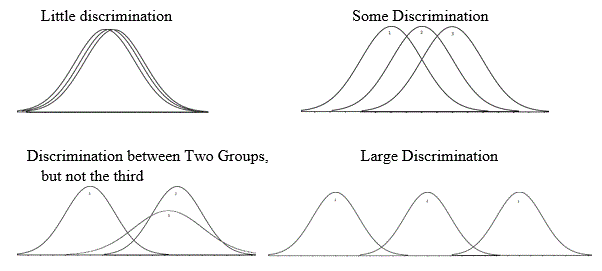
\includegraphics{wiki/2.png}
\caption{ss\_between}
\end{figure}

\begin{enumerate}
\def\labelenumi{\arabic{enumi}.}
\setcounter{enumi}{1}
\tightlist
\item
  Within-group variablity: It refers to variations caused by differences
  within individual groups as not all the values within each group are
  the same.
\end{enumerate}

high variability:

\begin{figure}
\centering
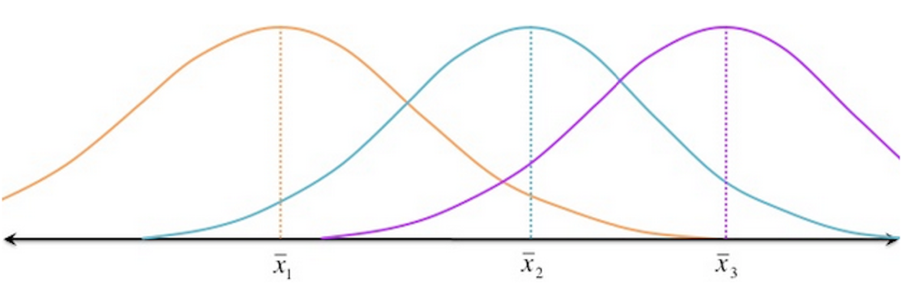
\includegraphics{wiki/3.png}
\caption{ss\_within}
\end{figure}

less variablity:

\begin{figure}
\centering
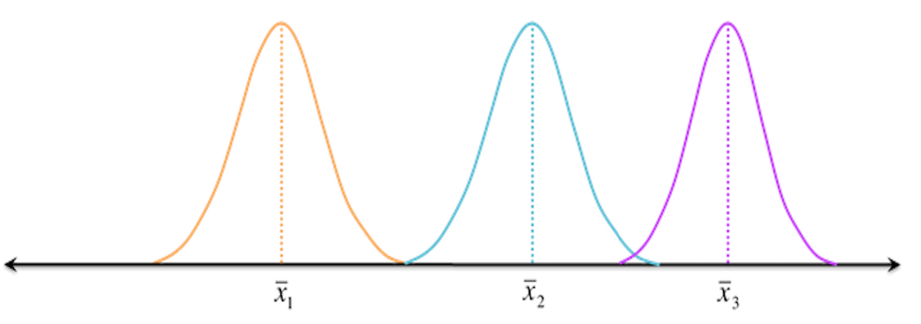
\includegraphics{wiki/4.png}
\caption{ss\_within}
\end{figure}

So as we can, both factors profoundly affect our decision to say that
two distribution (groups) are from same population or not.

Here are the steps: 1. Calculate mean of whole data =
\texttt{global\_mean} 2. Calculate mean of all samples within a group =
\texttt{group\_means} 3. Calculate between group variability: 1.
Calculate the sum of squared differences between group\_means and
global\_mean weighed with number of samples in each group =
\texttt{ss\_between} 2. Normalize ss\_between by defining
\texttt{df\_between} as the (number of groups - 1) 3. Calculate
normalized ss\_between by deviding it by df\_between =
\texttt{ms\_between} 4. Calculate within group variability: 1. Calculate
the sum of squared differences between each sample within a group from
its group mean = \texttt{ss\_within} 2. Normalize ss\_within by defining
\texttt{df\_within} as the (number of samples - number of groups) 3.
Calculate normalized ss\_within by deviding it by df\_within =
\texttt{ms\_within} 5. Calculate F-score 1. Calculate (ms\_between /
ms\_within) = \texttt{f\_score} 2. Find \texttt{f\_critical} from
F-table (F-ditribution) using df\_between as x-factor and df\_within as
y-factor (see
\href{https://www.dummies.com/education/math/business-statistics/how-to-find-the-critical-values-for-an-anova-hypothesis-using-the-f-table/}{Here})
3. If f\_score \textgreater{} f\_critical then there is a honest
significat difference between at least 2 groups.

Till now we just found out that there is a significant difference or
not. But what is the degree of difference between different groups or
simply which is better if they are different. To achieve the answer to
this question, all we need to do is using Tukey's HSD test.

    \begin{Verbatim}[commandchars=\\\{\}]
{\color{incolor}In [{\color{incolor}17}]:} \PY{n}{group\PYZus{}mean} \PY{o}{=} \PY{n}{all\PYZus{}acc}\PY{o}{.}\PY{n}{mean}\PY{p}{(}\PY{n}{axis}\PY{o}{=}\PY{l+m+mi}{0}\PY{p}{)}
         \PY{n}{global\PYZus{}mean} \PY{o}{=} \PY{n}{all\PYZus{}acc}\PY{o}{.}\PY{n}{mean}\PY{p}{(}\PY{p}{)}
         \PY{n}{n\PYZus{}groups} \PY{o}{=} \PY{n}{all\PYZus{}acc}\PY{o}{.}\PY{n}{shape}\PY{p}{[}\PY{l+m+mi}{1}\PY{p}{]}
         \PY{n}{n\PYZus{}instances} \PY{o}{=} \PY{n}{all\PYZus{}acc}\PY{o}{.}\PY{n}{shape}\PY{p}{[}\PY{l+m+mi}{0}\PY{p}{]}
         
         \PY{n}{f\PYZus{}threshold} \PY{o}{=} \PY{l+m+mf}{0.05}
         
         \PY{n}{ss\PYZus{}between} \PY{o}{=} \PY{n}{np}\PY{o}{.}\PY{n}{sum}\PY{p}{(}\PY{n}{n\PYZus{}instances} \PY{o}{*} \PY{p}{(}\PY{n}{group\PYZus{}mean} \PY{o}{\PYZhy{}} \PY{n}{global\PYZus{}mean}\PY{p}{)} \PY{o}{*}\PY{o}{*} \PY{l+m+mi}{2}\PY{p}{)}
         \PY{n}{df\PYZus{}between} \PY{o}{=} \PY{n}{n\PYZus{}groups} \PY{o}{\PYZhy{}} \PY{l+m+mi}{1}
         \PY{n}{ms\PYZus{}between} \PY{o}{=} \PY{n}{ss\PYZus{}between} \PY{o}{/} \PY{n}{df\PYZus{}between}
         
         \PY{n}{ss\PYZus{}within} \PY{o}{=} \PY{n}{np}\PY{o}{.}\PY{n}{sum}\PY{p}{(}\PY{p}{(}\PY{n}{all\PYZus{}acc} \PY{o}{\PYZhy{}} \PY{n}{group\PYZus{}mean}\PY{o}{.}\PY{n}{reshape}\PY{p}{(}\PY{l+m+mi}{1}\PY{p}{,} \PY{o}{\PYZhy{}}\PY{l+m+mi}{1}\PY{p}{)}\PY{p}{)} \PY{o}{*}\PY{o}{*} \PY{l+m+mi}{2}\PY{p}{)}
         \PY{n}{df\PYZus{}within} \PY{o}{=} \PY{n}{np}\PY{o}{.}\PY{n}{sum}\PY{p}{(}\PY{p}{[}\PY{n}{n}\PY{o}{\PYZhy{}}\PY{l+m+mi}{1} \PY{k}{for} \PY{n}{n} \PY{o+ow}{in} \PY{p}{[}\PY{n}{n\PYZus{}instances}\PY{p}{]}\PY{o}{*}\PY{n}{n\PYZus{}groups}\PY{p}{]}\PY{p}{)}
         \PY{n}{ms\PYZus{}within} \PY{o}{=} \PY{n}{ss\PYZus{}within} \PY{o}{/} \PY{n}{df\PYZus{}within}
         
         \PY{n}{f\PYZus{}score} \PY{o}{=} \PY{n}{ms\PYZus{}between} \PY{o}{/} \PY{n}{ms\PYZus{}within}
         \PY{n}{f\PYZus{}critical} \PY{o}{=} \PY{n}{f}\PY{o}{.}\PY{n}{ppf}\PY{p}{(}\PY{l+m+mi}{1}\PY{o}{\PYZhy{}}\PY{n}{f\PYZus{}threshold}\PY{p}{,} \PY{n}{df\PYZus{}between}\PY{p}{,} \PY{n}{df\PYZus{}within}\PY{p}{)}
         \PY{k}{if} \PY{n}{f\PYZus{}score} \PY{o}{\PYZgt{}} \PY{n}{f\PYZus{}critical}\PY{p}{:}
             \PY{n+nb}{print}\PY{p}{(}\PY{l+s+s1}{\PYZsq{}}\PY{l+s+s1}{There is huge difference between classes}\PY{l+s+s1}{\PYZsq{}}\PY{p}{)}
\end{Verbatim}


    \begin{Verbatim}[commandchars=\\\{\}]
There is huge difference between classes

    \end{Verbatim}

    \hypertarget{d-hsd}{%
\subsubsection{5.D HSD}\label{d-hsd}}

We want to find the difference degree between each two pair of groups.
To do so, HSD enables us to calculate it by values optained from ANOVA.

Note: HSD only works on ANOVA.

In the begining we said that ANOVA calculates that difference between
means of two groups are significant or not. In HSD, we are doing same
but for calculating this, we need to consider contriution of all samples
and other groups while calculating the difference between two mean and
this achieved by defining standard error of anova and normalizing each
mean difference of any pair of groups by dividing it by standard error
of anova.

Here are the steps: 1. Calculate standard error of ANOVA as square root
of normalized ms\_within = \texttt{se\_anova} 2. Traverse within all
unique pair of groups: 1. Divide difference of means of the pair and
divide it by se\_anova = \texttt{q} 2. If absolute value of q is bigger
than f\_critical then consider the difference as honest significant
difference 3. Report q as the difference

    \begin{Verbatim}[commandchars=\\\{\}]
{\color{incolor}In [{\color{incolor}19}]:} \PY{n}{columns} \PY{o}{=} \PY{p}{(}\PY{l+s+s1}{\PYZsq{}}\PY{l+s+s1}{AdaBoost}\PY{l+s+s1}{\PYZsq{}}\PY{p}{,} \PY{l+s+s1}{\PYZsq{}}\PY{l+s+s1}{RUSBoost}\PY{l+s+s1}{\PYZsq{}}\PY{p}{,} \PY{l+s+s1}{\PYZsq{}}\PY{l+s+s1}{SMOTEBoost}\PY{l+s+s1}{\PYZsq{}}\PY{p}{,} \PY{l+s+s1}{\PYZsq{}}\PY{l+s+s1}{RBBoost}\PY{l+s+s1}{\PYZsq{}}\PY{p}{,} \PY{l+s+s1}{\PYZsq{}}\PY{l+s+s1}{SVC}\PY{l+s+s1}{\PYZsq{}}\PY{p}{,} \PY{l+s+s1}{\PYZsq{}}\PY{l+s+s1}{RandomForest}\PY{l+s+s1}{\PYZsq{}}\PY{p}{)}
         \PY{n}{se\PYZus{}anova} \PY{o}{=} \PY{n}{np}\PY{o}{.}\PY{n}{sqrt}\PY{p}{(}\PY{n}{ms\PYZus{}within} \PY{o}{/} \PY{n}{n\PYZus{}instances}\PY{p}{)}
         
         \PY{n+nb}{print}\PY{p}{(}\PY{l+s+s1}{\PYZsq{}}\PY{l+s+s1}{Help1: Pos diff means first class is better and vice versa.}\PY{l+s+s1}{\PYZsq{}}\PY{p}{)}
         \PY{n+nb}{print}\PY{p}{(}\PY{l+s+s1}{\PYZsq{}}\PY{l+s+s1}{Help2: Higher diff means higher difference in performance and vice versa.}\PY{l+s+se}{\PYZbs{}n}\PY{l+s+s1}{\PYZsq{}}\PY{p}{)}
         \PY{k}{for} \PY{n}{i} \PY{o+ow}{in} \PY{n+nb}{range}\PY{p}{(}\PY{n}{n\PYZus{}groups}\PY{p}{)}\PY{p}{:}
             \PY{k}{for} \PY{n}{j} \PY{o+ow}{in} \PY{n+nb}{range}\PY{p}{(}\PY{n}{i}\PY{p}{,} \PY{n}{n\PYZus{}groups}\PY{p}{)}\PY{p}{:}
                 \PY{n}{q} \PY{o}{=} \PY{p}{(}\PY{n}{group\PYZus{}mean}\PY{p}{[}\PY{n}{i}\PY{p}{]} \PY{o}{\PYZhy{}} \PY{n}{group\PYZus{}mean}\PY{p}{[}\PY{n}{j}\PY{p}{]}\PY{p}{)} \PY{o}{/} \PY{n}{se\PYZus{}anova}
                 \PY{k}{if} \PY{n}{np}\PY{o}{.}\PY{n}{abs}\PY{p}{(}\PY{n}{q}\PY{p}{)} \PY{o}{\PYZgt{}} \PY{n}{f\PYZus{}critical}\PY{p}{:}
                     \PY{n+nb}{print}\PY{p}{(}\PY{l+s+s1}{\PYZsq{}}\PY{l+s+s1}{HSD Between \PYZhy{}\PYZhy{}\PYZhy{}\PYZgt{} }\PY{l+s+si}{\PYZob{}\PYZcb{}}\PY{l+s+s1}{ \PYZam{} }\PY{l+s+si}{\PYZob{}\PYZcb{}}\PY{l+s+s1}{ \PYZhy{}\PYZhy{}\PYZgt{} diff=}\PY{l+s+si}{\PYZob{}\PYZcb{}}\PY{l+s+s1}{\PYZsq{}}\PY{o}{.}\PY{n}{format}\PY{p}{(}\PY{n}{columns}\PY{p}{[}\PY{n}{i}\PY{p}{]}\PY{p}{,} \PY{n}{columns}\PY{p}{[}\PY{n}{j}\PY{p}{]}\PY{p}{,} \PY{n}{q}\PY{o}{\PYZhy{}}\PY{n}{f\PYZus{}critical}\PY{p}{)}\PY{p}{)}
\end{Verbatim}


    \begin{Verbatim}[commandchars=\\\{\}]
Help1: Pos diff means first class is better and vice versa.
Help2: Higher diff means higher difference in performance and vice versa.

HSD Between ---> AdaBoost \& SVC --> diff=-7.21928216231305
HSD Between ---> AdaBoost \& RandomForest --> diff=3.7705219977002473
HSD Between ---> RUSBoost \& SMOTEBoost --> diff=-5.0903672203209425
HSD Between ---> RUSBoost \& SVC --> diff=-8.139894029120427
HSD Between ---> RUSBoost \& RandomForest --> diff=2.8499101308928703
HSD Between ---> SMOTEBoost \& SVC --> diff=-5.435596670373702
HSD Between ---> SMOTEBoost \& RandomForest --> diff=5.554207489639596
HSD Between ---> RBBoost \& SVC --> diff=-5.78082612042646
HSD Between ---> RBBoost \& RandomForest --> diff=5.208978039586837
HSD Between ---> SVC \& RandomForest --> diff=8.603734298439083

    \end{Verbatim}

    Observations:

\begin{enumerate}
\def\labelenumi{\arabic{enumi}.}
\tightlist
\item
  AdaBoost has not HSD from its variant like SMOTEBoost. (weird - maybe
  because of bad sampling of 10 folds or ensemble size)
\item
  RUSBoost outperformed by other boosting with huge HSD.
\item
  RandomForest is worst
\item
  SVC is the best with highest HSD from all other methods.
\end{enumerate}


    % Add a bibliography block to the postdoc
    
    
    
    \end{document}
